\setcounter{chapter}{11}

\chapter{无穷级数}

无穷级数也就是{\kaishu 无穷和},数学上将其定义为{\kaishu 依序相加}的一列数或一列函数,
因为需要累加的项有无穷多,因此它本质上也是一类极限。

人类对于无穷级数认识首先来自于对数项级数的观察,例如{\kaishu 调和级数}和{\kaishu 等比级数},
然后逐渐扩充到更一般的数项级数。围绕数项级数的核心问题,常常不是如何
求它的和,而是判定它是否收敛(趋于某个确定的值)。根据级数构造的特点,
历史上,很多数学家提出过不同的判敛方法,也各有其应用的范围。
然而,不幸的是,并没有一种方法能够一劳永逸地解决所有的级数判敛问题,
因此,级数自人们发现它以来就一直是数学中的一项难题。

函数项级数是数项级数的推广,其中最典型的两类是{\kaishu 幂级数}和{\kaishu Fourier级数},
当然,它们远远不是全部。如果是一列函数(以正整数为下标)依序累加起来,
就可以称为函数项级数。

幂级数在分析学中具有无可替代的重要地位,因为拥有良好的可计算性和局部收敛性,
它广泛用于各种函数的展开和近似,是最基本和人类最熟悉的一类函数项级数。
与幂级数相关的知识延续了Taylor公式的有关理论,但对其的应用甚至早于微积分
理论的完整提出。

Fourier级数是在现代工程中有非常重要应用的函数项级数,特别是在信号处理
领域,离不开与其相关的许多工具,例如Fourier分析和Fourier变换
(Fourier Transformation,傅里叶变换)。

幂级数和Fourier级数在收敛特征上具有非常典型的差异,非常适合作为
后续学习和研究其他函数项级数的基础。深入地理解级数的本质,灵活和大胆地加以应用,
对于真正理解微积分,将其思想推广应用于更广阔的领域具有重要的意义。

\section{数项级数的概念与性质}

\subsection{数项级数的概念}

{\bf 数项级数}也称为{\bf 常数项级数},有时简称为{\bf 无穷级数}、{\bf 级数}
或{\bf 无穷和},直观地说,就是无穷多个数值的相加。

随着人们对无穷这一概念认识地深入,数学家们意识到,单纯地无穷个数相加,
要想得到确定的结果,有时也会以来其求和的次序,而且,就无穷本身而言,
更适合描述成一种从有限出发无限增长的过程,因此,用极限来定义级数就
成了级数概念严格化的基本途径。

在数学上,无穷级数就是指{\kaishu 某个数列按照其排列的顺序依次相加},也即:
\begin{thx}
	给定数列$\{a_n\}$,则其对应的{\bf 无穷级数}可定义为
	$$\sumn a_n=\limn\sum_{k=1}^na_k,$$
	其中$S_n=\limn\sum_{k=1}^na_k$称为其对应的{\bf 有限和}
	或{\bf 有限和数列}。若$\{S_n\}$收敛,则称该{\bf 无穷级数收敛},
	$\{S_n\}$的极限称为该{\bf 无穷级数的和};若$\{S_n\}$发散,
	则称该{\bf 无穷级数发散}。
\end{thx}

在这个定义中,引入极限决定了求和次序对于无穷级数的重要意义,
\ps{正确理解级数的定义是理解其各种性质的关键,严格来说,历史上正是由
对级数的研究启发人们创造了极限的概念,著名的例子包括割圆法和芝诺悖论}
如果改变求和次序(也即改变数列$\{a_n\}$的排列顺序),则相应地得到的
级数也被认为是不同的,即使它们可能都收敛到相同的和。

{\bf 例:}判断下列级数的收敛性
\begin{enumerate}[(1)]
  \setlength{\itemindent}{1cm}
  \item $\sumn q^n\quad (q>0)$ \quad({\it\b 几何级数,$|q|<1$时收敛}) 
  \item $\sumn\df{1}{n(n+1)}=1$\quad\ps{“裂项”——有理函数分解}
  \item $\sumn\df 1n$ \quad({\it\b 调和级数,发散})\\ 
  提示:$$S_{2n}-S_n=\df1{2n}+\df1{2n-1}+\ldots+\df1n
  >n\cdot\df1{2n}=\df12$$
  由此进而易知$\{S_n\}$无界,从而发散!
% 		  \item $\sumn\df 1n^2$
  \item $\sumn (-1)^n$ \quad({\it 发散})
\end{enumerate}

\begin{shaded}
{\bf 关于调和级数}

调和级数发散的速度慢得让人有些不可思议,其前$1000$项的和约为$7.485$,
前$100$万项的和约为$14.357$,前$10$亿项的和约为$21$,前一万亿项和约为$28$,
当它的和超过$100$时,如果每一项在纸带上只占$1$毫米,我们必须使用$10^{43}$毫米长
的纸带,这大约是$10^{25}$光年,而宇宙估计尺寸只有$10^{12}$光年,
因此也难怪大家都会认为它是收敛的。

{\bf Euler常数}

Euler常数最先由瑞士数学家莱昂哈德·欧拉(Leonhard Euler)
在1735年发表的文章 De Progressionibus harmonicus observationes 中定义。
欧拉曾经使用C作为它的符号,并计算出了它的前6位小数。1761年他又将该值计算到了16位小数。
$$\gamma=\limn\left[\sum\limits_{k=1}^n\df1k-\ln n\right]
=\int_1^{\infty}\left(\df1{[x]}-\df1x\right)\d x$$
由不等式$\ln(1+x)<x,(x\in(-1,+\infty),x\ne 0)$,
$$S_n=\sum\limits_{k=1}^n\df1k-\ln n>\sum\limits_{k=1}^n
\ln\left(1+\df1k\right)-\ln n=\ln(n+1)-\ln n>0.$$
$$S_n-S_{n+1}=\ln(n+1)-\ln n-\df1{n+1}>\left(\df1{n+1}\right)
-\df1{n+1}=0.$$
由单调有界原理可知$\{S_n\}$收敛。
\end{shaded}

\subsection{收敛级数的基本性质}

\begin{thx}
	\begin{enumerate}
	  \item {\bf 收敛的必要条件:}$\sumn a_n\mbox{收敛}\Rightarrow\limn a_n=0$
	  \begin{itemize}
	    \item 常用于判定级数发散:\b 若$\{a_n\}$不以$0$为极限,则$\sumn a_n$发散
	  \end{itemize}
	  \item {\bf 线性组合:}两个收敛级数的线性组合仍然收敛
	  \begin{itemize}
	    \item 问:一个收敛级数和一个不收敛的级数的线性组合是否收敛?
	  \end{itemize}
	  \item {\bf 改变有限项:}改变级数的有限项不改变其敛散性,例如: 
	  $\sumn a_n$收敛$\Leftrightarrow\sum\limits_{n=k}^{\infty}a_n$收敛$(k\in\mathbb{N})$
	  \begin{itemize}
	    \item 改变包括{\kaishu 修改、删除、添加};
	    \item 该性质等价于:修改数列的有限项不改变其敛散性;
	    \item 改变有限项后敛散性不变,但无穷和可能不同。
	  \end{itemize}
	  \item {\bf 合并收敛级数的相邻项}:任意合并收敛级数的相邻项,所得级数仍收敛
	  \begin{itemize}
	    \item 对于发散级数,该性质不成立,例如:$\sumn(-1)^n$
	    \item 改变求和次序,尽可能改变级数的敛散性,也可能改变级数的收敛和
	  \end{itemize}
	\end{enumerate}
\end{thx}

{\bf 例:}判断以下级数的敛散性;若收敛,求其和

\begin{enumerate}[(1)]
  \setlength{\itemindent}{1cm}
  \item $\sumn\ln\left(1+\df 1n\right)$
  \item
  $\sumn\left[\prod\limits_{k=0}^p(\alpha+n+k)\right]^{-1},\;(p\in\mathbb{N})$
  \item $\sumn\df{x^{2^{n-1}}}{1-x^{2n}}$
  \item $\sumn\df{1}{\sqrt n}$
\end{enumerate}

{\bf 例:}判断正误
\begin{enumerate}[(1)]
  \setlength{\itemindent}{1cm}
  \item $\{a_n\}$与$\sumn a_n$同敛散\hfill$\times$
  \item $k\ne 0$,则$\sumn a_n$与$\sumn ka_n$同敛散\hfill$\surd$
  \item $\sumn a_n$收敛,$\sumn b_n$发散,则$\sumn(a_n+b_n)$发散\hfill$\surd$
  \item $\sumn a_n$与$\sumn b_n$均发散,则$\sumn(a_n+b_n)$发散\hfill$\times$
  \item 若$\sum\limits_{n=1}^{\infty}a_{2n}$和
  $\sum\limits_{n=1}^{\infty}a_{2n-1}$均收敛,则$\sumn a_n$收敛\hfill$\surd$
  \item 若$\sum\limits_{n=1}^{\infty}(a_{2n}+a_{2n-1})$收敛,则
  $\sumn a_n$收敛\hfill$\times$
\end{enumerate}

\subsection{Cauchy审敛原理}

以下结论可以视为数列极限的Cauchy审敛原理的另一种表述:
\begin{thx}
	{\bf Cauchy审敛原理:}级数$\sumn a_n$收敛当且仅当:$\forall\e$,
    $\exists N\in\mathbb{Z}$,使对$\forall n>N$和$\forall p\in\mathbb{Z}^+$,
    都有
    $$|a_{n+1}+a_{n+2}+\ldots+a_{n+p}|<\e.$$
\end{thx}

{\bf 例:}证明:$\sumn\df1{n^2}$收敛。

[证]:注意到
\begin{align}
	&|a_{n+1}+a_{n+2}+\ldots+a_{n+p}|\notag\\
	&<\df1{(n+1)(n+2)}+\df1{(n+2)(n+3)}+\ldots+\df1{(n+p-1)(n+p)}\notag\\
	&=\df1n-\df1{n+p}<\df1n\notag
\end{align}
故由Cauchy审敛原则,易知该级数收敛。\fin

\begin{shaded}
	{\bf “好玩”的级数}
	
	级数的求和问题一直是非常“有趣”也非常困难的问题,关于级数$\sumn\df1{n^2}$
	的和,Euler给出了一个让人脑洞打开的解法:
	
	据说,是法国数学家François Viète(1540-1603)最早发现了代数方程
	的根与系数的关系,也即所谓的{\kaishu Viète定理},其最简单的形式如下:
	两个数$x_1,x_2$为一元二次方程$ax^2+bx+c=0$的根,当且仅当:
	$$x_1+x_2=-\df ba,\quad x_1x_2=\df ca.$$
	这个定理很容易被推广到一元$n$次多项式方程的情形:	$n$个数$x_1,x_2,\ldots,x_n$
	为一元$n$次多项式方程
	$$a_nx^n+a_{n-1}x^{n-1}+\ldots+a_1x+a_0=0$$
	的根,当且仅当同时成立如下的关系:
	\begin{align*}
		\sum\limits_{i=1}^nx_i&=-\df{a_{n-1}}{a_n}\\
		\sum\limits_{1\leq i<j\leq n}x_ix_j&=\df{a_{n-2}}{a_n}\\
		\ldots&\ldots\\
		\sum\limits_{1\leq i_1<i_2<\ldots<i_m\leq n}
		x_{i_1}x_{i_2}\ldots x_{i_m}&=(-1)^m\df{a_{n-m}}{a_n}\\
		\ldots&\ldots\\
		x_1x_2\ldots x_n&=(-1)^n\df{a_0}{a_n}.
	\end{align*}
	由这个结论出发,可以得出这样的结果
	$$\sum\limits_{i=1}^nx_i^2=\left(\sum\limits_{i=1}^nx_i\right)^2
	-2\sum\limits_{1\leq i<j\leq n}x_ix_j=\df{a_{n-1}^2-2a_na_{n-2}}{a_n^2}.$$
	假设所有的$x_i\ne0\;(i=1,2,\ldots,n)$,则不难发现$\df1{x_1},\df1{x_2},\ldots,
	\df1{x_n}$恰好为一元$n$次多项式方程
	$$a_0x^n+a_1x^{n-1}+\ldots+a_{n-1}x+a_n=0$$
	的全部根,从而就有
	$$\sum\limits_{i=1}^n\df1{x_i^2}=\df{a_1^2-2a_0a_2}{a_0^2}.$$
	通过学习Taylor公式,我们了解到对任意$x\in\mbb{R}$,都有
	$$\df{\sin x}x=1-\df{x^2}{3!}+\df{x^4}{5!}-\df{x^6}{7!}+\ldots,$$
	并且显然$\df{\sin x}x=0$的根为$x_i=\pm i\pi(i\in\mbb{N})$,于是Euler大胆地
	推测,此前关于一元$n$次多项式方程的根的结论应该也可以推广到无穷级数(相当于无穷次多项式)
	方程的情形,这样就有
	$$\sumn\df{2}{n^2\pi^2}=\df{0^2-2\left(-\df1{3!}\right)\cdot1}{1^2},$$
	稍加整理即得
	$$\sumn\df1{n^2}=\df{\pi^2}6.$$
	利用类似的方法,还可以证明
	$$\sumn\df1{n^4}=\df{\pi^4}{90}.$$
\end{shaded}

% {\bf 例:}求和$\sumn\df1{n(n+1)(n+2)}=\df14$。

{\bf 例:}求和$\sumn\df{n}{3^n}$。

[提示]:记$S_n=\df13+\df2{3^2}+\ldots+\df n{3^n}$,则
$$\df13S_n=\left(\df1{3^2}+\df2{3^3}+\ldots
+\df{n-1}{3^n}\right)+\df{n}{3^{n+1}}$$
因此
$$\df23S_n=\df12\left(1-\df1{3^n}\right)-\df{n}{3^{n+1}}\to\df12
(n\to\infty)$$

\begin{ext}
	{\bf 课后作业}
	\begin{enumerate}
	  \item 求以下级数的和
	  \begin{enumerate}[(1)]
	    \item $\df1{1\cdot6}+\df1{6\cdot11}+\df1{11\cdot16}+\ldots$
	    \item $\df1{1\cdot2\cdot3}+\df1{2\cdot3\cdot4}+\df1{3\cdot4\cdot5}+\ldots$
	    \item $\sumn\df{n}{(n+1)!}$
	  \end{enumerate}
	  \item 已知$\sumn(a_{2n-1}+a_{2n})$收敛,能否推出$\sumn a_n$收敛?
	  如果能,请给出证明;如果不能,请给出反例,并讨论还需要增加什么条件才能够由
	  前者推出后者。
	  \item (选作)利用Cauchy审敛原理判定如下级数的敛散性
	  \begin{enumerate}[(1)]
	    \item $\sumn\df{(-1)^{n}}n$
	    \item $\sumn\df{\sin nx}{2^n}$
	  \end{enumerate}
	\end{enumerate}
\end{ext}

\section{数项级数的审敛法}

给定一个数项级数,如果能够直接求出其和,或者利用求和来判断
其是否收敛,当然是非常理想的结果。但是由于级数问题的复杂性,
在现实中,想要采用某种统一的方法简单地得到级数的和,往往难以
实现。事实上,单就判定一个级数的敛散性问题本身已经是非常具有
挑战性了。

为了研究级数的审敛问题,我们首先从比较特殊的级数问题出发,
先来讨论级数每一项都非负或非正的情形(称为{\kaishu 同号级数}),
特别地,以下就以所谓的{\kaishu 正项级数}(各项都非负)为例
给出一系列判别敛散性的方法。

\subsection{正项级数审敛法}

\subsubsection{收敛的充要条件}

\begin{thx}
	{\bf 正项级数收敛的充要条件:}正项级数收敛,当且仅当其部分和数列有界。
\end{thx}

[证]:设$\sumn a_n$为正项级数,$\{S_n\}$为其部分和数列,显然
$\{S_n\}$单调递增,由已知$\{S_n\}$有界,故由单调有界原理,
$\{S_n\}$收敛,也即$\sumn a_n$收敛。\fin

显然,该定理相当于数列收敛的单调有界原理的一种不同的表述。

{\bf 例:}证明$\sumn\df1{n!}$收敛。

[证]:设$\{S_n\}$为该级数的部分和数列,则对任意$n>2$,都有
\begin{align*}
	S_n&=1+\df12+\df1{3!}+\ldots+\df1{n!}\\
	&<1+\df12+\df1{2^2}+\ldots+\df1{2^{n-1}}<2,
\end{align*}
从而由正项级数收敛的充要条件,该级数收敛。\fin

\subsubsection{比较判别法}

\begin{thx}
	{\bf 比较判别法的(不等式形式)}:若对充分大的$n$,总有$0\leq a_n\leq b_n$,则
	\begin{enumerate}
% 	  \setlength{\itemindent}{1cm}
	  \item 若$\sumn b_n$收敛,则$\sumn a_n$收敛
	  \item 若$\sumn a_n$发散,则$\sumn b_n$发散
	\end{enumerate}
\end{thx}

[证]:不妨设对任意的$n$,均有$0\leq a_n\leq b_n$。
设$\{S_n^1\}$,$\{S_n^2\}$分别为$\sumn a_n$和$\sumn b_n$的
部分和数列,显然$0\leq S_n^1\leq S_n^2$,因此,由数列收敛的
夹逼准则,若$\{S_n^2\}$收敛,则$\{S_n^1\}$收敛,也即
若$\sumn b_n$收敛,则$\sumn a_n$收敛。反之,若$\{S_n^1\}$
发散,则$\{S_n^2\}$发散,也即若$\sumn a_n$发散,则$\sumn b_n$发散。\fin

通过以上证明,不难看出,这个定理可以视为数列极限的夹逼准则的
一种不同的表述。

需要注意的是,{\b 对于变号(非同号)级数,比较判别法是不成立的},例如:
$$a_n=-\df1n+\df{(-1)^n}{\sqrt n}<\df{(-1)^n}{\sqrt n}=b_n,$$
学习了交错级数的Leibniz判别法后,我们可以证明$\sumn b_n$收敛,
但$\sumn a_n$是发散的。

{\bf 例:}证明:$p$-级数$\sumn\df1{n^p}$,
\ps{$p$-级数常常用作与其他级数比较判敛的“标杆”}
\begin{enumerate}[(1)]
  \setlength{\itemindent}{1cm}
  \item 当$p>1$时,收敛;
  \item $0<p\leq 1$时,发散。
\end{enumerate}

[证]:
\begin{shaded}
(1)由以下推导可知$p>1$时,$p$-级数的部分和数列有界
\begin{eqnarray*}
	S_{(2^k)^p}&=&1+\df 1{2^p}+\underbrace{\left(\df1{3^p}+\df1{(2^2)^p}\right)}_2
				+\underbrace{\left(\df1{5^p}+\ldots+\df1{(2^3)^p}\right)}_{2^2}+\ldots\\
				&&+\underbrace{\left[\df1{(2^{k-1}+1)^p}+\ldots+\df1{(2^k)^p}\right]}_{2^{k-1}}\\
			  &\leq &1+\df 1{2^p}+2\cdot\df1{2^p}+2^2\cdot\df1{(2^2)^p}
			    +\ldots+2^{k-1}\cdot\df1{(2^{k-1})^p}\\
			  &=&1+\df 1{2^p}+\left[\df1{2^{p-1}}+\left(\df1{2^{p-1}}\right)^2+
			    \ldots+\left(\df1{2^{p-1}}\right)^{k-1}\right]\\
			  &=&1+\df 1{2^p}+\df1{2^{p-1}}\df{1-\left(\frac1{2^{p-1}}\right)
			    ^{k-1}}{1-\frac1{2^{p-1}}}<1+\df 1{2^p}+\df1{2^{p-1}-1}
\end{eqnarray*}
\end{shaded}

(1)证明$p>1$时$p$-级数收敛更好的方法是利用其与无穷积分的联系,具体请参加
第五章的反常积分一节。

(2),$p=1$时,显然发散。又因为
$$0<\df 1n<\df 1{n^p},\quad (0<p<1),$$
已知调和级数发散,故由比较判别法,此时$p$-级数发散。\fin

{\bf 例:}讨论下列级数的敛散性
\begin{enumerate}[(1)]
  \setlength{\itemindent}{1cm}
  \item $\sumn\df{1}{3^{\ln n}}$
  \hfill({[提示]:$a^{\ln b}=b^{\ln a},\;(a,b>0)$})
  \item $\sum\limits_{n=2}^{\infty}\df 1{(\ln n)^{\ln n}}$
  \item $\sum\limits_{n=3}^{\infty}\df 1{(\ln n)^{\ln\ln n}}$
\end{enumerate}
	
[提示]: (2)\;当$n>e^{e^2}$时,
$$(\ln n)^{\ln n}=n^{\ln\ln n}>n^2.$$

(3)\;注意到$n$充分大时,$\ln n<\sqrt{n}$,进而$(\ln\ln n)^2<\ln n$,故有
  $$\df 1{(\ln n)^{\ln\ln n}}=\df 1{e^{(\ln\ln
  n)^2}}>\df 1n$$

\begin{shaded}
	{\bf\color{red} 一点“常识”}
	
	{\color{red} 设$\e>0, a>1$,则对于充分大的$x$,总成立如下关系
	$$\ln x<<x^{\e}<<a^x<<[x]!<<x^x$$}

	这些结论使用L'Hospital法则都可以很容易地证明。
	
	{\bf 例:} 对于充分大的$x$,$e^x>2x^4$,故对充分大的$n$,
	有$e^{\sqrt[3]n}>2n^{\frac 43}$,从而可知$\sumn e^{-\sqrt[3]n}$收敛
\end{shaded}

需要注意的是,虽然在非正向级数的情况下,仅仅由$a_n\leq b_n$,无法推出
$\sumn b_n$收敛则$\sumn a_n$收敛的结论,但存在如下一种特殊的情况,
其形式更类似于数列极限的夹逼定理:

\begin{thx}
	设当$n$充分大时,$a_n\leq c_n\leq b_n$,$\sumn a_n,\sumn
	b_n$均收敛, 则$\sumn c_n$收敛。
\end{thx}

[证]:构造新的级数$\sumn(c_n-a_n)$和$\sumn(b_n-a_n)$,则
这两个级数满足比较判别法的条件,从而易知结论成立。\fin

注意到对任意的级数$\sumn a_n$,总有
$$-|a_n|\leq a_n\leq |a_n|,$$
故由以上的结论立刻可以得到如下的推论:

\begin{thx}
	{\bf 绝对值级数收敛,则原级数必收敛:}若级数$\sumn|a_n|$收敛,则$\sumn a_n$也收敛。
\end{thx}

有些情况下,可在对正向级数$\sumn a_n$和$\sumn b_n$作比较时,可以
考虑其各项值的极限,相对于不等式放缩,计算极限通常可能更加简单:

\begin{thx}
	{\bf 比较判别法(极限形式):}已知$a_n,b_n$均非负$(n\in\mathbb{Z}_+)$,
	且$\limn\df{a_n}{b_n}=l$,则 
	\begin{enumerate}
% 	  \setlength{\itemindent}{1cm}
	  \item 若$0<l<+\infty$,$\sumn a_n,\sumn b_n$同敛散 \hfill({\it\b 随着$n$的增大,
	  $a_n,b_n$的比值趋于常数})
	  \item 若$l=0$,由$\sumn b_n$收敛可知$\sumn a_n$收敛; 
	  \hfill({\it\b 随着$n$的增大,$a_n$的值远小于$b_n$})
	  \item 若$l=+\infty$,由$\sumn a_n$收敛可知$\sumn b_n$收敛
	  \hfill({\it\b 随着$n$的增大,$a_n$的值远大于$b_n$})
	\end{enumerate}
\end{thx}

[证]:1. 设$0<l<+\infty$,由$\limn\df{a_n}{b_n}=l$,对
$\e=\df l2$,存在$N\in\mbb{Z}_+$,使对任意$n>N$,都有
$\left|\df{a_n}{b_n}-l\right|<\e$,也即
$$\df l2b_n<a_n<\df{3l}2b_n.$$
若$\sumn b_n$收敛,则$\sumn\df{3l}2b_n$收敛,进而
$\sum\limits_{n=N+1}^{\infty}\df{3l}2b_n$收敛,
由以上右端不等式可知,$\sum\limits_{n=N+1}^{\infty}a_n$收敛,
从而$\sumn a_n$收敛。

同理可证,若$\sumn b_n$发散,则$\sumn a_n$发散。综上,当
$0<l<+\infty$时,$\sumn a_n,\sumn b_n$同敛散。

2. 设$l=0$,由$\limn\df{a_n}{b_n}=0$,对$\e=1$,存在
$N\in\mbb{Z}_+$,使对任意$n>N$,都有
$\left|\df{a_n}{b_n}\right|<\e$,也即
$$a_n<b_n.$$
若$\sumn b_n$收敛,则$\sum\limits_{n=N+1}^{\infty}b_n$收敛,
由以上右端不等式可知,$\sum\limits_{n=N+1}^{\infty}a_n$收敛,
从而$\sumn a_n$收敛。

3. 若$l=+\infty$,由$\limn\df{a_n}{b_n}=+\infty$可得
$\limn\df{b_n}{a_n}=0$,利用上一部分的结论即可。\fin

{\bf 例:}判断以下级数的敛散性:
\begin{enumerate}[(1)]
  \setlength{\itemindent}{1cm}
  \item $\sumn\df 1{2^n}\df{n^2+1}{2n^2-1}$ 
  \item $\sumn\df{n+1}{n^k+2}\quad (k=1,2,\ldots)$ 
  \item $\sumn\df{1}{n\sqrt[n]{n}}$ 
  \item $\sumn\df{1}{1+x^n}\quad(x>0)$
\end{enumerate}

显然,应用比较判别法的关键,是要找到作为参照的“标杆”。考虑到$p$-级数的
敛散性是非常明确的,而且其表达形式也比较简单,很多时候,在比较判别法中
会以之为“标杆”来来判定其他级数的敛散性。

\begin{thx}
	{\bf $p$-判别法:}设$a_n\geq 0\;(n=1,2,\ldots)$,则 
	\begin{enumerate}
% 	  \setlength{\itemindent}{1cm}
	  \item 若存在$p>1$,使得$\limn n^pa_n$存在,则$\sumn a_n$收敛 
	  \item 若$0<p\leq 1$,使得$\limn n^pa_n>0$,则$\sumn a_n$发散
	\end{enumerate}
\end{thx}

{\bf 例:}判断以下级数的收敛性
\begin{enumerate}[(1)]
  \setlength{\itemindent}{1cm}
  \item $\sumn\df{\arctan n}{n^{3/2}}$
  \item $\sumn\df{\ln n}{n^{5/4}}$\ps{任何正幂次函数的增长速度最终都比任意对数函数快}
\end{enumerate}

{\bf 例:}$\sumn a_n$、$\sumn b_n$均为正项级数,若对充分大的$n$,总有
$$\df{a_{n+1}}{a_n}\leq\df{b_{n+1}}{b_n},$$
则若$\sumn b_n$收敛,$\sumn a_n$收敛。

[证]:由已知,存在$N\in\mbb{Z}_+$,使对任意$n>N$有
$$\df{a_{n+1}}{a_n}\leq\df{b_{n+1}}{b_n},$$
进而
$$a_{n+1}
\leq\df{b_{n+1}}{b_n}a_n
\leq\df{b_{n+1}}{b_n}\df{b_{n}}{b_{n-1}}a_{n-1}
=\df{b_{n+1}}{b_{n-1}}a_{n-1}
\leq\ldots
\leq\df{b_{n+1}}{b_{N+1}}a_{N+1}
=\df{a_{N+1}}{b_{N+1}}b_{n+1}.$$
因为$\sumn b_n$收敛,故$\sum\limits_{n=N+1}^{\infty}b_n$收敛,
进而由比较判别法可知,$\sum\limits_{n=N+1}^{\infty}a_n$收敛,
再有收敛级数的性质可知,$\sumn a_n$收敛。\fin

{\bf 例:}(2012年全国大学生数学竞赛)
$\sumn a_n$和$\sumn b_n$均为正项级数,证明:
\begin{enumerate}[(1)]
  \setlength{\itemindent}{1cm}
  \item 若$\limn\left(\df{a_n}{a_{n+1}b_n}-\df 1{b_{n+1}}\right)>0$,
  则$\sumn a_n$收敛;
  \item 若$\limn\left(\df{a_n}{a_{n+1}b_n}-\df 1{b_{n+1}}\right)<0$,
  且$\sumn b_n$发散,则$\sumn a_n$发散。
\end{enumerate}

[证]:(1)由已知,存在$q>0$和$N\in\mathbb{Z}_+$,对任意$n\geq N$,有
$$\df{a_n}{a_{n+1}b_n}-\df 1{b_{n+1}}>q,$$
从而
$$a_{n+1}<\df1q\left(\df{a_n}{b_n}-\df{a_{n+1}}{b_{n+1}}\right).$$
利用递推关系可得
$$\sum\limits_{k=N}^na_k<a_N+\df1q\left(\df{a_N}{b_N}-\df{a_n}{b_n}\right)
<a_N+\df1q\df{a_N}{b_N},$$
故$\sumn a_n$部分和有界,从而收敛。

(2)$n$充分大($n>N$)时,有
$$a_{n+1}>\df{b_{n+1}}{b_n}a_n>\ldots>
\df{b_{n+1}}{b_n}\df{b_{n}}{b_{n-1}}\ldots\df{b_{N+1}}{b_N}a_N
=\df{a_N}{b_N}b_{n+1},$$
由比较判别法,$\sumn b_n$发散,则$\sumn a_n$发散。\fin

{\bf 例:} 判断以下级数是否收敛:$\sumn\left(\cot\df{n\pi}{4n-2}-\sin\df{n\pi}{2n+1}\right)$

[解]:考虑$\sumn\left(1-\cot\df{n\pi}{4n-2}\right)$和
$\sumn\left(1-\sin\df{n\pi}{2n+1}\right)$,注意到
$$\limn\df{1-\cot\df{n\pi}{4n-2}}{\df1n}=\df{\pi}4,
\quad\limn\df{1-\sin\df{n\pi}{2n+1}}{\df1{n^2}}=\df{\pi^2}{32},$$
故以上级数一个发散一个收敛,从而原级数发散。\fin

比较判别法是正项级数审敛的最基本方法,后续所有的判别法可以说都是它的推论。
但是相对来说,比较判别法并不是一个特别容易使用的方法,因为使用它判别级数的
敛散性时,不仅需要找到合适的“标杆”,还需要事先“猜测”出最终的敛散性,
而所谓的“标杆”只是用于验证猜测的结果。为了更好地“猜测”级数的敛散,对于
各种函数形式值的“大小”的判断是关键,为此我们前面提到的那一点“常识”
和对各种数列极限结论的熟练掌握就非常重要了。

最后,请务必牢记{\bf\color{red}比较判别法仅对同号级数有效!!!}

\subsubsection{比值判别法}

比值判别法也叫{\kaishu d'Alembert判别法}。

\begin{thx}
	{\bf 比值判别法(极限形式)}
	设$a_n\geq 0(n=1,2,\ldots)$,$\limn\df{a_{n+1}}{a_n}=q$,则
	\begin{enumerate}
% 	  \setlength{\itemindent}{1cm}
	  \item $0\leq q<1$时,$\sumn a_n$收敛; 
	  \item $q>1$时,$\sumn a_n$发散。
	\end{enumerate}
\end{thx}

[证]:若$q>1$,极限的保号性,存在$N\in\mbb{Z}_+$,使当
$n>N$时,$\df{a_{n+1}}{a_n}>1$,也即$a_{n+1}>a_n$,
这与级数收敛的必要条件$\limn a_n=0$矛盾,从而此时$\sumn a_n$发散。

若$0\leq q<1$,记$p=\frac{1+q}2$,
由极限的保号性,存在$N\in\mbb{Z}_+$,使当
$n>N$时,$\df{a_{n+1}}{a_n}<p$,从而
$$a_{n+1}<p{a_n}<p^2a_{n-1}<\ldots<p^{n+1-N}a_{N+1},$$
进而
$$\sum\limits_{k=N+1}^{n}a_k<(1+p+p^2+\ldots+p^{n-1})a_{N+1}
<\df1{1-p}a_{N+1},$$
由此可知$\sumn a_n$的部分和有界,从而$\sumn a_n$收敛。\fin

{\bf 注:}$q=1$时,比值判别法无法给出确定的结论,也即{\kaishu 无法判定},
例如:$\sumn\df 1n$和$\sumn\df 1{n^2}$都对应于$q=1$,但前者发散,后者收敛。

{\bf 例:}判断下列级数的收敛性
\begin{enumerate} [(1)]
  \setlength{\itemindent}{1cm}
  \item $\sumn\df 1{2^n}\df{n^2+1}{2n^2-1}$ 
  \item $\sumn\df{n^2}{2^n}$ 
  \item $\sumn\df{(2n)!}{(n!)^2}$
%   \item $\sumn n!\left(\df{x}{n}\right)^n\quad (x>0)$
\end{enumerate}

{\bf 例:}设$t>0$,讨论级数$\sumn\df{t^nn!}{n^n}$的敛散性。

[提示]:若$t=e$,
$$\df{a_{n+1}}{a_n}=\df{e}{\left(1+\df1n\right)^n}>1,$$
故$\{a_n\}$必不以$0$为极限,可知$\sumn a_n$发散;

$t\ne e$的情况利用比值判别法即可判断。

{\bf 思考:}考虑$\sumn\df{n^n}{e^nn!}$,
则以上推导不再成立,该如何判定其敛散性呢?

[提示]:因为$\left(1+\df1n\right)^n<e<\left(1+\df1n\right)^{n+1}$,故
$$\df{a_{n+1}}{a_n}=\df{\left(1+\df1n\right)^n}{e}>\df1{1+\frac1n}=\df n{n+1},$$
于是
$$a_n>\df{n-1}na_{n-1}>\df{n-1}n\cdot\df{n-2}{n-1}\ldots\df12a_1=\df{a_1}n,$$
由此易知原级数发散。

\begin{thx}
	{\bf 比值判别法(不等式形式)}设$a_n\geq 0\,(n=1,2,\ldots)$,则 
	\begin{enumerate}
% 	  \setlength{\itemindent}{1cm}
	  \item 若$n$充分大时,有$\df{a_{n+1}}{a_n}\leq r<1$,则$\sumn a_n$收敛; 
	  \item 若$n$充分大时,有$\df{a_{n+1}}{a_n}\geq 1$,则$\sumn a_n$发散。
	\end{enumerate}
\end{thx}

该定理的证明可以完全参照极限形式的证明进行。

{\b {\bf 思考:}为什么以上第一个判定条件中要求$r<1$?

{\bf 答:}因为若仅要求$\df{a_{n+1}}{a_n}<1$,不能避免出现
$\limn\df{a_{n+1}}{a_n}=1$的情况,从而导致无法判定。}

{\bf 例:}判断以下级数的收敛性$\sumn\df{2+(-1)^n}{5^n}$。

[提示]:本例适合使用根植判别法,或者比值判别法的不等式形式

{\bf 例:} 判断以下级数的收敛性:$\sqrt2+\sqrt{2-\sqrt2}+\sqrt{2-\sqrt{2-\sqrt2}}
+\sqrt{2-\sqrt{2-\sqrt{2-\sqrt2}}}$

[解]:
$$\sqrt2=2\cos\df{\pi}4=2\sin\df{\pi}4$$
$$\sqrt{2-\sqrt2}=\sqrt{2\left(1-\cos\df{\pi}4\right)}=2\sin\df{\pi}8$$
$$\sqrt{2-\sqrt{2-\sqrt2}}=\ldots=2\sin\df{\pi}{16}$$
故$a_n=2\sin\df{\pi}{2^{n+1}}$。记$b_n=\df{\pi}{2^{n}}$,注意到
$$\limn\df{a_n}{b_n}=1,$$
且$\sumn b_n$收敛,故原级数收敛。\fin

\subsubsection{根值判别法}

根值判别法也叫{\kaishu Cauchy判别法}

\begin{thx}
	{\bf 根植判别法(极限形式):}设$a_n\geq 0(n=1,2,\ldots)$,$\limn\sqrt[n]{a_n}=q$,则
	\begin{enumerate}
% 	  \setlength{\itemindent}{1cm}
	  \item $0\leq q<1\Rightarrow\sumn a_n$收敛
	  \item $q>1\Rightarrow\sumn a_n$发散
	\end{enumerate}
\end{thx}

和比值法类似,$q=1$时,无法判定级数的敛散性。

此外,需要注意的是,由数列极限的性质:
$\limn\df{a_{n+1}}{a_n}=q\Rightarrow\limn\sqrt[n]{a_n}=q$,
\ps{参见第一章介绍的Stolz定理}
故我们可以知道根植判别法相对于比值判别法的应用范围要更广一些。


{\bf 例:}判断下列级数的收敛性
\begin{enumerate} [(1)]
  \setlength{\itemindent}{1cm}
  \item $\sumn\df{2+(-1)^n}{5^n}$
  \item $\sumn\df{n^2}{\left(2+\df 1n\right)^n}$
  \item $\df 12+\df 1{3^2}+\df 1{2^3}+\df 1{3^4}+\df 1{2^5}+\df 1{3^6}+\ldots$
\end{enumerate}

% {\bf EX:}$a_n=\df{n^{n+\frac1n}}{\left(n+\df1n\right)^n}
% \geq\df{n^n\cdot n^{\frac1n}}{(n+1)^n}\to\df1e$
% hence $\sumn\df{n^{n+\frac1n}}{\left(n+\df1n\right)^n}$ diverge

{\bf 思考:}根植判别法的不等式形式该如何表述?

{\bf 例:}判断下列级数的收敛性
\begin{enumerate} [(1)]
  \setlength{\itemindent}{1cm}
  \item $\sumn\df1{3^n}\left[\sqrt2+(-1)^n\right]^n$
  \item $\sumn\df{n^{n+\frac1n}}{\left(n+\df1n\right)^n}$\\
  提示:$\df{n^{n+\frac1n}}{\left(n+\df1n\right)^n}\geq\df{n^n\cdot
  n^{\frac1n}}{(n+1)^n}\to\df1e\ne0$,故发散。
\end{enumerate}

另解:
$$\limn\df{n^{n+\frac1n}}{\left(n+\df1n\right)^n}
=\limn\df{\sqrt[n]n}{\left(1+\df1{n^2}\right)^n},$$
其中
$$\limn\left(1+\df1{n^2}\right)^n=
\left\{\limn\left(1+\df1{n^2}\right)^{n^2}\right\}^{\limn\frac1n}=e^0=1,$$
故以上极限$=1\ne0$,级数不满足收敛的必要条件!

\begin{shaded}

\subsubsection{其他判别法}

以上我们介绍的是最常用的正项级数审敛法,除了它们之外,还有许多“有趣”
的判别法,例如:

\begin{tcolorbox}
	{\bf Raabe判别法(极限形式):}设$a_n\geq 0\,(n=1,2,\ldots)$,且
	$$\limn n\left(\df{a_n}{a_{n+1}}-1\right)=r,$$
	则当$r>1$时,$\sumn a_n$收敛;$r\leq 1$时,$\sumn a_n$发散。	
\end{tcolorbox}

{\bf 例:}判断以下级数的敛散性
\begin{enumerate}[(1)]
  \setlength{\itemindent}{1cm}
  \item $\sumn\df{(2n-1)!!}{(2n)!!}\df 1{2n+1}$
  \item $\sumn\df{n!}{(x+1)\ldots(x+n)}\;(x>0)$
  \item $\sumn\df{p(p+1)\ldots(p-n+1)}{n!n^q}$
  \item $\df ab+\df{a(a+d)}{b(b+d)}++\df{a(a+d)(a+2d)}{b(b+d)(b+2d)},(a,b,d>0)$
\end{enumerate}

[提示]:(1)
$$R_n=n\left[\df{(2n+2)(2n+3)}{(2n+1)(2n+1)}-1\right]
=\df{n(6n+5)}{(2n+1)^2}\to\df32>1\;(n\to\infty)$$
(2)
$$R_n=n\left[\df{n+x}{n+1}-1\right]=\df{n(x-1)}{n+1}$$

\begin{tcolorbox}
	{\bf Raabe判别法(不等式形式):}设$a_n\geq 0\,(n=1,2,\ldots)$,定义
	$$R_n=n\left(\df{a_n}{a_{n+1}}-1\right),$$
	若存在$r>1$,当$n$充分大时,总有$R_n\geq r$,则$\sumn a_n$收敛;
	若当$n$充分大时,总有$R_n\leq 1$,则$\sumn a_n$发散。	
\end{tcolorbox}

{\bf 例:}判断以下级数的敛散性
$$\sumn\df{\sqrt{n!}}{(2+\sqrt 1)(2+\sqrt 2)\ldots(2+\sqrt n)}$$

[提示]:记$a_n=\df{\sqrt{n!}}{(2+\sqrt 1)(2+\sqrt 2)\ldots(2+\sqrt n)}$,
从而
$$n\left(\df{a_n}{a_{n+1}}-1\right)=\df{2n}{\sqrt{n+1}}\to\infty\;(n\to\infty)$$
从而易知该级数收敛。

\begin{tcolorbox}
	{\bf Bertrand判别法:}$\{a_n\}$非负,
	$$\limn\ln n\left[n\left(\df{a_n}{a_{n+1}}-1\right)-1\right]=b,$$
	则:$b>1$时,$\sumn a_n$收敛;$b<1$时,发散。
\end{tcolorbox}

\begin{tcolorbox}
	{\bf Gauss判别法:}$\{a_n\}$非负,
	$$\df{a_n}{a_{n+1}}=1+\df{\mu}n+\mathrm{O}\left(\df1{n^{1+\e}}\right),\;\e>0,$$
	则:$\mu>1$时,$\sumn a_n$收敛;$\mu<1$时,发散。
\end{tcolorbox}

\begin{tcolorbox}
	{\bf 对数判别法:}	$\{a_n\}$非负,
	\begin{enumerate}
	  \item $\limn\df{\ln\df1{a_n}}{\ln n}=r,$
		则:$r>1$时,$\sumn a_n$收敛;$r<1$时,发散。
	  \item  $\limn\df{\ln\df1{na_n}}{\ln\ln n}=r,$
		则:$r>1$时,$\sumn a_n$收敛;$r<1$时,发散。
	\end{enumerate}	
\end{tcolorbox}

{\bf 例:}证明级数$\sumn\left(\df{\sqrt n}{1+\sqrt n}\right)^n$收敛。

\begin{tcolorbox}
	{\bf Cauchy积分判别法:}设$f(x)$在$x\geq 1$上单调递减,
	则$\sumn f(n)$和$\dint_1^{+\infty}f(x)\d x$同敛散。
\end{tcolorbox}

\begin{tcolorbox}
	{\bf Sapagof判别法:}$\{a_n\}$单调趋于零,当且仅当
	$\sumn\left(1-\df{a_{n+1}}{a_n}\right)$发散。
\end{tcolorbox}
\end{shaded}

\subsection{交错级数审敛法}

{\bf 交错级数:}相邻各项符号相反的级数,例如:设$a_n\geq 0,(n\in\mathbb{Z}_+)$,则
$$\sumn(-1)^na_n$$
为交错级数。

\begin{thx}
	{\bf Leibniz判别法:}若数列$\{a_n\}$单调趋于$0$,则交错级数$\sumn (-1)^na_n$收敛,且
	其和的绝对值不超过$|a_1|$。
\end{thx}

必须注意的是{\b Leibniz判别法只是一个充分条件,将其作为必要条件使用是最常见的一种错误!}
例如:$\df12-\df13+\df1{2^2}-\df1{3^2}+\df1{2^3}-\df1{3^3}+\ldots$收敛,
但其通项去绝对值后并不具有单调性。

{\bf 例:}判断下列级数的敛散性
\begin{enumerate} [(1)]
  \setlength{\itemindent}{1cm}
  \item $\sumn(-1)^{n-1}\df{2^nn!}{n^n}$ 
  \item $\sumn(-1)^n\df{\sqrt{n}}{n+100}$\hfill{($n>100$时$a_n$单调递减趋于$0$)}
  \item $\sumn\sin\left(\pi\sqrt{n^2+k^2}\right),(k\in\mathbb{Z}_+)$
\end{enumerate}

{\bf 例:} 设$a_n=(-1)^n\ln\left(1+\df1n\right)$,是否 
$\sumn a_n$和$\sumn a^2_n$均收敛?

[提示]:$\left\{\ln\left(1+\df1n\right)\right\}$单调递减趋于零,
故由Leibniz判别法,$\sumn a_n$收敛。

注意到\ps{$\df1{n+1}<\ln\left(1+\df1n\right)<\df1n$}
$$0<\ln\left(1+\df1n\right)<\df1n\quad\Rightarrow\quad
\left[\ln\left(1+\df1n\right)\right]^2<\df1{n^2},$$
由比较判别法,级数$\sumn a^2_n$收敛。

{\bf 思考:}{\b 若级数$\sumn a_n$收敛,$\sumn a^2_n$必收敛?}

答:错!若$a_n$均非负,由级数收敛的必要条件,必有$\limn a_n=0$,
从而可知,当$n$充分大时,必有$a_n<1$,进而有$0<a^2_n<a_n$,由比较
判别法,级数$\sumn a^2_n$收敛。\ps{也可以利用比较法的极限形式:$\limn\df{a^2_n}{a_n}=0$}

但若$a_n$可能变号,以上结论将不再成立。事实上,存在反例:$a_n=(-1)^n\df1{\sqrt n}$

% {\bf 例:}求和
% \begin{enumerate}[(1)]
%   \setlength{\itemindent}{1cm}
%   \item $\sum\limits_{n=2}^{\infty}\df{(-1)^n}{\sqrt n+(-1)^n}
%   =\df{(-1)^n\sqrt n}{n-1-\df1{n-1}}$
%   \item $\sum\limits_{n=2}^{\infty}\df{(-1)^n}{\sqrt{n+(-1)^n}}
%   =\left(\df1{\sqrt 3}-\df1{\sqrt 2}\right)+\left(\df1{\sqrt 5}-\df1{\sqrt
%   4}\right)+\ldots+\left(\df1{\sqrt{2n+1}}-\df1{\sqrt{2n}}\right)$
% \end{enumerate}
% 
% $$\df1{\sqrt{2n+1}}-\df1{\sqrt{2n}}=-\df1{\sqrt{2n(2n+1)}
% (\sqrt{2n}+\sqrt{2n+1})}$$

\subsection{绝对收敛和条件收敛}

Leibniz判别易于使用,但是其局限性也是显而易见的,对于非交错级数的
变号级数而言,它是完全无能为力的。

有时候,对于一个变号级数,要判定其收敛,可以通过判定其各项取绝对值
之后的级数收敛来实现。这种加了各项绝对值之后所得级数仍收敛的性质称为
{\bf 绝对(值)收敛},否则,如果原级数收敛,但不绝对收敛,则称为
{\bf 条件收敛}。

\begin{thx}
	{\bf 绝对收敛的性质:}
	\begin{enumerate}
	  \item {\kaishu 绝对收敛的级数必收敛:}若$\sumn |a_n|$收敛,则$\sumn a_n$收敛;反之不然;
	  \item {\kaishu 交换律:}绝对收敛级数求和项任意交换次序其无穷和不变;
	  \item {\kaishu 级数的Cauchy乘积:}设$\sumn a_n,\sumn
	  b_n$绝对收敛,则$\sum\limits_{i,j=1}^na_ib_j$绝对收敛,且
	  $$\sum\limits_{i,j=1}^{\infty}a_ib_j=\sumn a_n\sumn b_n$$
	\end{enumerate}
\end{thx}

{\b{\bf 注意:}绝对收敛和条件收敛都可以推出$\sumn a_n$收敛!}

{\bf 例:}已知$0\leq a_n\leq\df1n$,以下哪个级数必收敛?\hfill(D)

\quad(A)\;$\sumn a_n$\quad(B)$\sumn (-1)^na_n$
\quad(C)$\sumn \sqrt{a_n}$\quad(D)$\sumn (-1)^na^2_n$

\begin{shaded}

\subsection{特殊判别法}

下面这些判别法仅作为了解即可:

\begin{tcolorbox}
	{\bf Dirichlet判别法:}若数列$\{a_n\}$单调趋于$0$,$\sumn b_n$
  	的部分和有界,则$\sumn a_nb_n$收敛。
\end{tcolorbox}
  
{\bf 例:}判断以下级数的敛散性
$$\sumn\df{\sin nx}n$$

[提示]:
设$a_n=\df1n,b_n=\sin nx$,注意到
\begin{eqnarray*}
&&\sin\df x2(\sin x+\sin2x+\cdots+\sin nx)\\
&=&\df12\left[\left(\cos\df x2-\cos\df{3x}2\right)+
\left(\cos\df {3x}2-\cos\df{5x}2\right)+\cdots+
\left(\cos\df {2n-1}2x-\cos\df{2n+1}2x\right)\right]\\
&=&\df12\left(\cos\df{x}2-\cos\df{2n+1}2x\right),
\end{eqnarray*}
故对给定$x$
$$\left|\sum\limits_{i=1}^n\sin ix\right|
\leq\df{\left|\cos\df{3x}2-\cos\df{2n+1}2x\right|}{2\left|\sin\df x2\right|}
\leq\df1{\left|\sin\df x2\right|},$$
有界。

又由
$$\left|\df{\sin nx}n\right|\geq\df{\sin^2nx}n=\df1{2n}-\df{\cos2nx}{2n},$$
且$\sumn\df1{2n}$发散,$\sumn\df{\cos2nx}{2n}$收敛,可知
$$\sumn\df{\sin nx}n$$是条件收敛的。

\begin{tcolorbox}
	{\bf Abel判别法:}若数列$\{a_n\}$单调有界,$\sumn b_n$收敛,
	则$\sumn a_nb_n$收敛。
\end{tcolorbox}

{\bf 例:}判断以下级数的敛散性

$$\sumn(-1)^n\left(1+\df 1n\right)^n\df{1}{\sqrt n}$$ 

\subsection{条件收敛的有趣性质}

一个变号级数若收敛,但又不绝对收敛,则会出现以下这样一个“令人惊讶”的性质:

\begin{tcolorbox}
	{\bf Riemann定理:}若级数$\sumn a_n$条件收敛,则对任意给定的数$A$,
	都可以通过对该级数的重新排列,使得新的级数以$A$为其和。
\end{tcolorbox}
这个定理意味着:
\begin{itemize}
  \item 对条件收敛的级数进行重排可能改变其和;
  \item 重排后的级数可能发散。
\end{itemize}

\end{shaded}

\begin{ext}
	{\bf 课后作业}
	\begin{enumerate}
	  \item 判断以下级数的敛散性,如果是收敛的变号级数,说明其是绝对收敛还是条件收敛:
	  \begin{enumerate}[(1)]
	    \item $\sumn\df{n-2}{3n^2+n}$
	    \item $\sumn\df{\sqrt{n+2}-\sqrt{n}}{\sqrt{n+1}}$
	    \item $\sumn\df{4^n}{n\cdot 3^n}$
	    \item $\sumn\df{n^2}{3^n}$
	    \item $\sumn\df1n\arctan\df1{n-1}$
	    \item $\sumn\left(\df{n}{2n-1}\right)^{3n+2}$
	    \item $\sumn n\left(\df34\right)^n$
	    \item $\sumn\df{n^2}{n!}$
	    \item $\sumn\df{n^{n+\frac1n}}{\left(1+\df1n\right)^n}$
	    \item $\sumn(-1)^n\df{2^n}{n!}$
	    \item $\sumn\sin\left(\pi\sqrt{n^2+1}\right)$
	    \item $\sumn\dint_0^{\frac{\pi}n}\df{\sin x}{1+x}\d x$
	    \item $\sumn\df{2^n-n^2}{3^n}$
	    \item $\sumn\df1{n\ln^2(n+1)}$
	  \end{enumerate}
	  \item 判断以下命题的正误,如果正确,证明之;如果错误,请给出反例,并讨论
	  需要添加什么条件方能使之成立:
	  \begin{enumerate}[(1)]
	    \item 已知级数$\sumn a_n$收敛,则级数$\sumn a^2_n$收敛;
	    \item 已知级数$\sumn a^2_n$收敛,则级数$\sumn a^3_n$收敛;
	    \item 正项级数$\sumn a_n$与级数$\sumn\df{a_n}{1+a_n}$同敛散;
	    \item 对于正项级数$\sumn a_n$,若当$n$充分大时,总有$\df{a_{n+1}}{a_n}<1$,
	    则该级数收敛。
	  \end{enumerate}
	\end{enumerate}
\end{ext}

\section{幂级数及其应用}

函数项级数是对常数项级数的推广,将原来由对确定数列的依序求和改为
对确定函数序列的依序求和,从这个意义上说,其实质并无不同。
例如,给定一个函数序列$\{u_n(x)\}$,其中$x\in I$为自变量,
对应的{\bf 函数项级数}定义为:
$$\sumn u_n(x)=\limn\sum\limits_{k=1}^nu_k(x),$$
其中$S_n(x)=\sum\limits_{k=1}^nu_k(x)$表示序列前$n$项的和,称为
其{\bf 部分和}(或{\bf 部分和函数})。如果对任意$x\in I$,
$\{S_n(x)\}$都收敛,记$S(x)=\limn S_n(x)$,则称
$S(x)$为以上函数项级数的{\bf 和函数}。能够使某个函数项级数收敛的
$x$的最大变化范围(区间)称为该函数项级数的{\bf 收敛域}。

本章我们主要介绍两类函数项级数:幂级数(power series)和Fourier级数。

\subsection{幂级数的概念与性质}

幂级数是一类形式简单而应用广泛的函数项级数,
其中变量可以是一个或多个(称为{\kaishu 多元幂级数})。
单变量(一元)的幂级数形如:
$$\sumn[0]a_n(x-x_0)^n,$$
其中的$x_0$和$a_0,a_1,\ldots,a_n,\ldots$都是常数。该级数通常称为
{\bf 关于$(x-x_0)$的幂级数}(或{\bf 以$x_0$为中心的幂级数}
\ps{幂级数也常被称为{\bf Taylor级数},特别是如果$x_0=0$,
也称为{\bf Maclaurin级数}})。

幂级数是分析学研究的重点之一,其最常见的用途是用来表示各种具有良好
解析性质(可导、可微)的函数,事实上,局部上由收敛幂级数给出的函数
被称为{\kaishu 解析函数},而我们接触的所有的初等函数都是解析函数。

以下的讨论中,我们通常假设$x_0=0$,以
$${\sum\limits_{n=0}^{\infty}a_nx^n}$$
为代表研究幂级数的有关性质。

对于一般形式的幂级数
$$\sumn[0]a_n(x-x_0)^n,$$
利用变换$y=x-x_0$,总可以将其化为与以上级数相同的形式,相应地,
其各种性质都可以间接地得到。

{\bf 例:}讨论如下幂级数的{\kaishu 收敛区间}:
\begin{enumerate}[(1)]
  \setlength{\itemindent}{1cm}
  \item $\sum\limits_{n=0}^{\infty}\df{x^n}{n!}$\hfill $(-\infty<x<+\infty)$
  \item $\sum\limits_{n=0}^{\infty}x^n$\hfill $(|x|<1)$
  \item $\sum\limits_{n=0}^{\infty}n!x^n$ \hfill $(x=0)$
\end{enumerate}

{\bf 注:}{\b 幂级数总是在某个(而不是多个)非空的区间上收敛,
且在忽略区间端点的情况下,该区间关于$x_0$对称。}

\begin{thx}
	{\bf Abel定理:}考虑幂级数
	$$\sum\limits_{n=0}^{\infty}a_nx^n$$
	\begin{enumerate}%[(1)]
% 	  \setlength{\itemindent}{1cm}
	  \item 若在$x_0\ne 0$处该级数收敛,则对任意$|x|<|x_0|$,该级数绝对收敛; 
	  \item 若在$x_0\ne 0$处该级数发散,则对任意$|x|>|x_0|$,该级数发散。 
	\end{enumerate}
\end{thx}

[分析]:考虑结论1。因为$x_0\ne 0$,故
$$|a_nx^n|=\left|a_nx_0^n\right|\left|\df{x}{x_0}\right|^n.$$
若已知级数在$x_0$处收敛,则由级数收敛的必要条件,必有
$\limn a_nx_0^n=0$,进而根据数列极限的性质(有界性),存在$M>0$,使对充分大的$n$,总有
$$\left|a_nx_0^n\right|<M.$$
至此可以看出当$n$充分大时,
$$|a_nx^n|<M\left|\df{x}{x_0}\right|^n.$$
上式右端的无穷和是一个几何(等比)级数,当$|x|<|x_0|$时,公比小于$1$,级数
收敛。于是由比较判别法,上式左端的无穷和也必收敛,也即此时原级数是绝对收敛的。

结论2与结论1等价,利用反证法容易证明。

Abel定理告诉我们这样一个事实:{\kaishu 对幂级数而言,在比某个收敛的点更靠近
级数中心的点上,级数必收敛;在比某个发散的点更远离级数中心的点上,级数必发散!}因此,
可以得到如下关于幂级数收敛区间的如下推论:

\begin{thx}
	{\bf 幂级数的收敛域:}存在收敛与发散的临界点:$x^*=\pm R$,使得幂级数在
	以$x_0$为中心$R$为半径({\bf 收敛半径})的对称开区间({\bf 收敛区间})内收敛,
	在其外发散。	
\end{thx}

由于上面的结论并未涉及收敛区间的端点,故{\b 在区间端点处的敛散性需要单独判定!}

{\bf 例:}设幂级数$\sumn a_nx^n$的收敛半径为$R=3$,求$\sumn a_n(x-1)^{n+1}$
的收敛区间。

[解]:记$y=x-1$,则$\sumn a_n(x-1)^n=\sumn a_ny^n$,由已知,右端级数
收敛半径为$3$,收敛区间为$y\in(-3,3)$,对应地,级数$\sumn a_n(x-1)^n$的
收敛区间为$x\in(-2,4)$。

又$\sumn a_n(x-1)^{n+1}=(x-1)\sumn a_n(x-1)^n$,注意到当$x-1\ne 0$
时,左右两端的级数之比为常数,故同敛散;又当$x-1=0$时,二者均收敛,故左端级数
的收敛区间与右端级数的收敛区间相同,也为$(-2,4)$。\fin

从上面这个例子的分析过程我们可以推出如下的结论:

\begin{thx}
	{\bf 幂级数的性质}:对任意$k\in\mbb{Z}^+$,幂级数$\sumn a_nx^n$与$\sum a_nx^{n+k}$的
	收敛区间相同。
\end{thx}

{\bf 例:}设$a_n\geq0\;(n\in\mathbb{N})$,证明:
若级数$\sum\limits_{n=0}^{\infty}a_n(x-x_0)^n$在$x_1$
处条件收敛,则其收敛半径$R=|x_1-x_0|$。

[证]:该级数在$x_1$收敛,则可知其收敛半径至少为$|x_1-x_0|$。又其对应的绝对值
级数$\sum\limits_{n=0}^{\infty}a_n|(x_1-x_0)|^n$发散,由此可知,其收敛半径
不可能大于$|x_1-x_0|$。\fin

{\bf 例:}设$a_n\geq0\;(n\in\mathbb{N})$,若$\sum a_n(x-2)^n$在$x=-2$收敛,
则在$x=5$处\underline{\;{绝对收敛}\;};若在$x=-2$处条件收敛,
则收敛半径为\underline{\;{$4$}\;}

\begin{thx}
	{\bf 幂级数的收敛半径:}若$\sum\limits_{n=0}^{\infty}a_nx^n$的系数满足
	$$\limn\left|\df{a_{n+1}}{a_n}\right|=\rho
	\quad\mbox{或}\quad\limn\sqrt[n]{|a_n|}=\rho,$$
	则该幂级数的收敛半径$R=1/\rho$。
\end{thx}

{\bf 例:}求下列幂级数的收敛域
\begin{enumerate}[(1)]
  \setlength{\itemindent}{1cm}
  \item $\sum\limits_{n=0}^{\infty}\df{2+(-1)^n}{2^n}x^n$
  \item $\sum\limits_{n=0}^{\infty}\df{(x-1)^n}{2^nn}$
  \item $\sum\limits_{n=0}^{\infty}2^nx^{2n}$
  \item $\sum\limits_{n=0}^{\infty}x^{3n+1}$
\end{enumerate}

[提示]:(1)收敛半径$R=2$,区间端点对应的级数均发散,故收敛域为$(-1,1)$;

(2)收敛半径$R=2$,$x=-1$时对应级数收敛,故收敛域为$[-1,1)$;

(3)令$u=x^2$,易得$|u|<1$时级数收敛,从而$|x|<1$为收敛域;

(4)原级数即为$x\sum\limits_{n=0}^{\infty}x^{3n}$,显然与
$\sum\limits_{n=0}^{\infty}x^{3n}$同敛散。令$u=x^3$,后一级数
即为$\sum\limits_{n=0}^{\infty}u^n$,收敛区间$|u|<1$。
最终可得原级数的收敛域为$|x|<1$。

关于求幂级数收敛半径和收敛域的步骤,可以简单总结如下:

\begin{thx}
	{\bf 求幂级数的收敛域:}
	\begin{enumerate}
% 	  \setlength{\itemindent}{1cm}
	  \item 一般步骤:{\b 先求收敛半径,再讨论区间端点的敛散性}
	  \item 标准型幂级数: $\sum\limits_{n=0}^{\infty}a_nx^n$ 
	  $$R=\limn\left|\df{a_n}{a_{n+1}}\right|
	  \quad\mbox{或}\quad R=\df 1{\limn\sqrt[n]{|a_n|}}$$ 
	  \item 非标准型幂级数(缺项或通项为复合函数):先换元、整理,再求收敛半径 
	  \item 比值极限不存在时,注意使用根值极限({\b 若
	  $\limn\left|\df{a_{n+1}}{a_n}\right|$存在,
	  $\limn\sqrt[n]{|a_n|}$必存在且与之相等})
	\end{enumerate}
\end{thx}

{\bf 例:}判断正误
\begin{enumerate}[(1)]
  \setlength{\itemindent}{1cm}
  \item 幂级数在其收敛域上一定绝对收敛
  \item 设$\sumn[0] a_nx^n,\sumn[0] b_nx^n$的收敛半径分别为$R_1,R_2$,
  则$\sumn[0](a_n+b_n)x^n$的收敛半径$R=\min\{R_1,R_2\}$ 
%   \item 幂级数与其逐项积分和逐项求导的幂级数的收敛域相同 
  \item 若$\sumn[0] a_nx^n$的收敛半径为$R$,则必有
  $$R=\limn\left|\df{a_n}{a_{n+1}}\right|
  \quad\mbox{或}\quad R=\df 1{\limn\sqrt[n]{|a_n|}}$$
\end{enumerate}

[提示]:(1)错!

正确的说法:幂级数在其收敛{\kaishu\b 区间}上一定绝对收敛!

(2)错!例如:$a_n=-b_n$,则$R=+\infty$;

又比如:设$a>1$,考虑$a_n=\df{a^nx^n}{1+a^n},b_n=\df{x^n}{1+a^n}$,
此时$R_1=1,R_2=\df1a<1,R=1$。

正确的说法:设$\sumn[0] a_nx^n,\sumn[0] b_nx^n$的收敛半径分别为$R_1,R_2$,
则$\sumn[0](a_n+b_n)x^n$的收敛半径$R${\kaishu\b 不小于}$\min\{R_1,R_2\}$。 

% (3)错!需要提出收敛域的端点!

(3)错!考虑级数$\sumn[0]\df{x^{2n}}{2^{2n}}+\sumn[0]2^{2n+1}x^{2n+1}$。

{\bf 思考:}证明:幂级数$\sumn[0]a_nx^n$和$\sumn[0]na_nx^n$的收敛区间相同。

[证]:设$\sumn[0]a_nx^n$的收敛区间为$(-R,R)$。任取$x_1\in(-R,R)$,对任意
$|x|<|x_1|$,有
$$|na_nx^n|=|a_nx_1^n|n\left|\df{x}{x_1}\right|^n,$$
可以证明$\limn n\left|\df{x}{x_1}\right|^n=0$,故由比较判别法,$\sumn[0]na_nx^n$
收敛,由$x$的任意性,可知$\sumn[0]na_nx^n$在$(-R,R)$上收敛。

以下证明$\sumn[0]na_nx^n$当$|x|>R$时均发散,用反证法。设存在$|x_2|>R$,使
$\sumn[0]na_nx^n$收敛,则对任意满足$|x|\in(R,|x_2|)$的$x$,
$$|a_nx^n|=|na_nx^n|\df1n\left|\df{x}{x_2}\right|^n,$$
可以证明$\limn\df1n\left|\df{x}{x_2}\right|^n=0$,故由比较判别法,可知
此时$\sumn[0]a_nx^n$收敛,从而与已知矛盾。

综上即证。\fin

\begin{thx}
	{\bf 幂级数的运算性质:}
	考虑幂级数$\sumn[0]a_nx^n$,设其和函数为$S(x)$,则
	\begin{enumerate}
% 	  \setlength{\itemindent}{1cm}
	  \item $S(x)$在该级数的收敛域上连续;
	  \item $\sumn[0]a_nx^n$在其收敛域上可逐项积分,即:
	  $$\b \dint_0^xS(t)\d t=\dint_0^x\left[\sumn[0]a_nt^n\right]\d t
	  =\sumn[0]\dint_0^xa_nt^n\d t=\sumn[0]\df{a_n}{n+1}x^{n+1},$$
	  \item $\sumn[0]a_nx^n$在其收敛可逐项求导,即:
	  $$\b S'(x)=\left(\sumn[0]a_nx^n\right)'
	  =\sumn[0](a_nx^n)'=\sumn na_nx^{n-1}.$$
	\end{enumerate}
\end{thx}

以上性质的证明请参考{\kaishu 同济大学教材第十二章第六节“函数项级数的一致收敛性及
一致收敛级数的基本性质”}或{\kaishu 数学分析}的相关教材。

\subsection{幂级数的和函数}

{\bf 例:}已知
$$\df{1}{x+1}=\sum\limits_{n=0}^{\infty}(-x)^n\;(|x|<1),$$
求幂级数
$$\sum\limits_{n=1}^{\infty}\df{(-1)^{n-1}}{n}x^n$$
的和函数。由此证明:
$$\ln 2=1-\df 12+\df 13-\df 14+\ldots+\df{(-1)^n}{n}+\ldots$$

[解]:所给幂级数的收敛域为$(-1,1]$。设其和函数为$S(x)$,则当$x\in(-1,1)$时,
\begin{align*}
	S'(x)&=\left[\sum\limits_{n=1}^{\infty}(-1)^{n-1}\df{x^n}{n}\right]'
	=\sum\limits_{n=1}^{\infty}\left[(-1)^{n-1}\df{x^n}{n}\right]'\\
	&=\sum\limits_{n=1}^{\infty}(-x)^{n-1}
	=\sum\limits_{n=0}^{\infty}(-x)^{n}=\df1{x+1},\quad x\in(-1,1),
\end{align*}
于是
$$S(x)=\dint_0^x\df1{t+1}\d t+S(0)=\ln|x+1|, \quad x\in(-1,1)$$
即为所求。又$S(x)$在$(-1,1]$上连续,故当$x=1$时,
$$1-\df 12+\df 13-\df14+\ldots+\df{(-1)^n}{n}+\ldots
=S(1)=\limx{1^-}S(x)=\ln 2.$$
\fin

{\bf 例:}求下列幂级数的和函数
\begin{enumerate}[(1)]
  \setlength{\itemindent}{1cm}
  \item $\sum\limits_{n=0}^{\infty}\df{x^n}{n!}$
  \item $\sum\limits_{n=1}^{\infty}nx^n$
  \item $\sum\limits_{n=0}^{\infty}\df{x^n}{n+1}$
  \item $\sum\limits_{n=0}^{\infty}n^2x^n$
\end{enumerate}

[提示]:(1)收敛域$(-\infty,+\infty)$,
$$S'(x)=\left[\sum\limits_{n=0}^{\infty}\df{x^n}{n!}\right]'
=\sum\limits_{n=0}^{\infty}\left[\df{x^n}{n!}\right]'
=\sum\limits_{n=1}^{\infty}\df{x^{n-1}}{(n-1)!}=S(x),$$
又$S(0)=1$,求解微分方程初值问题,可得$S(x)=e^x$。

(2)收敛域$(-1,1)$,
$$
	\df{S(x)}x=\sum\limits_{n=1}^{\infty}nx^{n-1}
	=\sum\limits_{n=1}^{\infty}(x^{n})'
	=\left(\sum\limits_{n=1}^{\infty}x^{n}\right)'
	=\left(\df1{1-x}-1\right)'=\df1{(1-x)^2},
$$
从而
$$S(x)=\df{x}{(1-x)^2},\quad x\in(-1,1)$$

(3)收敛域$[-1,1)$,
$$
xS(x)=\sum\limits_{n=0}^{\infty}\df{x^n+1}{n+1}
=\sum\limits_{n=0}^{\infty}\dint_0^x t^n\d t
=\dint_0^x \sum\limits_{n=0}^{\infty}t^n\d t
=\dint_0^x \df1{1-t}\d t=-\ln|1-x|,
$$
故
$$S(x)=\left\{\begin{array}{ll}
	-\df{\ln|1-x|}x,&x\ne0\\
	1,&x=0.
\end{array}\right.$$
\fin

{\bf 例:}求幂级数$\sumn[0]\df{(-1)^n}{(n+1)2^n}x^{n+1}$。\ps{课堂练习}

[提示]:$\ln(2+x)-\ln2$,$x\in(-2,2]$。

{\bf 例:}求数项级数$\sumn\sum\limits_{k=1}^n\df{k}{2^{n-1}}$的和。

[提示]:\ps{交换求和次序,可以使用初等方法求得级数的和}原级数即为
$$\sumn\df{n(n+1)}{2^n}.$$
考虑幂级数$\sumn n(n+1)x^n$,求出其和函数,然后令$x=\df12$即可。

\subsection{函数的幂级数展开}

函数$f(x)$在原点处的无穷阶Taylor展开式:
$$f(x)=\sum\limits_{n=0}^{\infty}\df{f^{(n)}(0)}{n!}x^n$$
 称为:{\kaishu $f(x)$在原点处的Taylor级数(Maclaurin级数)}

{\bf 注:}展开的条件: $f(x)$在原点处无穷阶可导。

\begin{thx}
	{\bf 常用的Maclaurin级数}
	\begin{enumerate}
	  \item $e^x=\sumn[0]\df{x^n}{n!},\;x\in(-\infty,+\infty)$
	  \item $\sin x=\sumn[0]\df{x^{2n+1}}{(2n+1)!},\;x\in(-\infty,+\infty)$
	  \item $\cos x=\sumn[0]\df{x^{2n}}{(2n)!},\;x\in(-\infty,+\infty)$
	  \item $\df1{1-x}=\sumn[0]x^n,\;x\in[-1,1)$
	  \item $\df1{1+x}=\sumn[0](-1)^nx^n,\;x\in(-1,1]$
	  \item $\ln(1+x)=\sumn[0]\df{(-1)^n}{n+1}x^{n+1},\;x\in(-1,1]$
	  \item $(1+x)^a=\sumn[0]\left(\begin{array}{c}
	  	a \\ n
	  \end{array}\right)x^n,\;x\in(-1,1)$
	\end{enumerate}
\end{thx}

一般函数的幂级数展开,可以求Taylor公式的方法进行,可能用到的技巧包括:

\begin{thx}
	{\bf 幂级数展开的常用方法}
	
	若在开区间$I$内,$f(x)=\sumn[0]a_nx^n$,
	$g(x)=\sumn[0]b_nx^n$,则对任意$x\in I$,
	\begin{enumerate}[(1)]
% 	  \setlength{\itemindent}{1cm}
	  \item {\it 变量替换:}
	  $$f(u)=\sumn[0]a_nu^n$$
	  \item {\it 线性性:}对任意$\lambda,\mu\in\mathbb{R}$,
	  $$\lambda f(x)+\mu g(x)=\sumn[0](\lambda a_n+\mu
	  b_n)x^n$$ 
	  \item {\it 逐项求导:}
	  $$f'(x)=\sumn[0]na_{n}x^{n-1}$$ 
	  \item {\it 逐项积分:} 
	  $$\dint_0^x f(t)\d t=\sum\limits_{n=0}^{\infty}
	  \df{a_{n}}{n+1}x^{n+1}$$
	\end{enumerate}
\end{thx}

{\bf 例:}求以下函数的Maclaurin级数

\begin{enumerate}[(1)]
  \setlength{\itemindent}{1cm}
  \item $f(x)=1+x+4x^3-5x^{99}+x^{100}$
  \item $f(x)=(1-x)e^x$
  \item $f(x)=\sin(x-\pi/4)$
  \item $f(x)=\df 1{1-x^2}$
  \item $f(x)=\ln(2+x)$
  \item $f(x)=\arctan x$
\end{enumerate}

[提示]:(1)关于$x$的多项式函数的Maclaurin级数就是其自身。

注:若要求在$x=a$处的Taylor级数,则需要将$x$代换为$(x-a)+a$,然后将
原多项式展开为关于$x-a$的多项式即可。

(2)
$$(1-x)e^x=\sum\limits_{n=0}^{\infty}(1-x)\df{x^n}{n!}
=1+\sum\limits_{n=1}^{\infty}\left[\df1{n!}-\df1{(n-1)!}\right]x^n
=1-\sum\limits_{n=1}^{\infty}\df1{n(n-2)!}x^n$$
收敛域$(-\infty,+\infty)$.

(3)
$$\sin(x-\pi/4)=\df{\sqrt2}2(\sin x-\cos x)
=\df{\sqrt2}2\sum\limits_{m=0}^{\infty}(-1)^m
\left(-\df{x^{2m}}{(2m)!}+\df{x^{2m+1}}{(2m+1)!}\right)$$
收敛域$(-\infty,+\infty)$.

(4)记$u=x^2$
$$\df 1{1-x^2}=\df1{1-u}=\sum\limits_{n=0}^{\infty}u^n
=\sum\limits_{n=0}^{\infty}x^{2n},$$
收敛域$(-1,1)$.

(5)记$u=\df x2$,则
$$\ln(2+x)=\ln2+\ln(1+u)
=\ln2+\sum\limits_{n=0}^{\infty}\df{(-1)^n}{n+1}u^{n+1}
=\ln2+\sum\limits_{n=0}^{\infty}\df{(-1)^n}{(n+1)2^n}x^{n+1},$$
收敛域$(-2,2]$

(6)由
$$\df1{1+x^2}=\sum\limits_{n=0}^{\infty}(-1)^nx^{2n},$$
两边同时积分,可得
$$\arctan x=\dint_0^x\left[\sum\limits_{n=0}^{\infty}(-1)^nt^{2n}\right]\d t
=\sum\limits_{n=0}^{\infty}(-1)^n\dint_0^xt^{2n}\d t
=\sum\limits_{n=0}^{\infty}\df{(-1)^n}{2n+1}x^{2n+1},$$
收敛域$(-1,1)$\ps{注意到$\arctan x$在$(-\infty,+\infty)$上处处无穷可导,但
其幂级数展开的收敛域只是$(-1,1)$,这很好地说明了幂级数的局部收敛性}

\begin{shaded}
	{\bf 关于$\arctan x$的展开的讨论}

	1、先来看$\arctan x$的幂级数展开。由
	$$(\arctan x)'=\df1{1+x^2}
	=\sum\limits_{n=0}^{\infty}(-1)^nx^{2n}, \quad (|x|<1),$$
	两边积分
	$$\arctan x=\dint_0^x\sum\limits_{n=0}^{\infty}(-1)^nt^{2n}\d t
	+\arctan 0
	=\sum\limits_{n=0}^{\infty}(-1)^n\dint_0^xt^{2n}\d t+0
	=\sum\limits_{n=0}^{\infty}\df{(-1)^n}{2n+1}x^{2n+1},$$
	以上右侧的幂级数的收敛域为$[-1,1]$。故
	$${\b\arctan x=\sum\limits_{n=0}^{\infty}\df{(-1)^n}{2n+1}x^{2n+1},
	\quad |x|\leq1}$$

	\begin{center}
		\resizebox{!}{5cm}{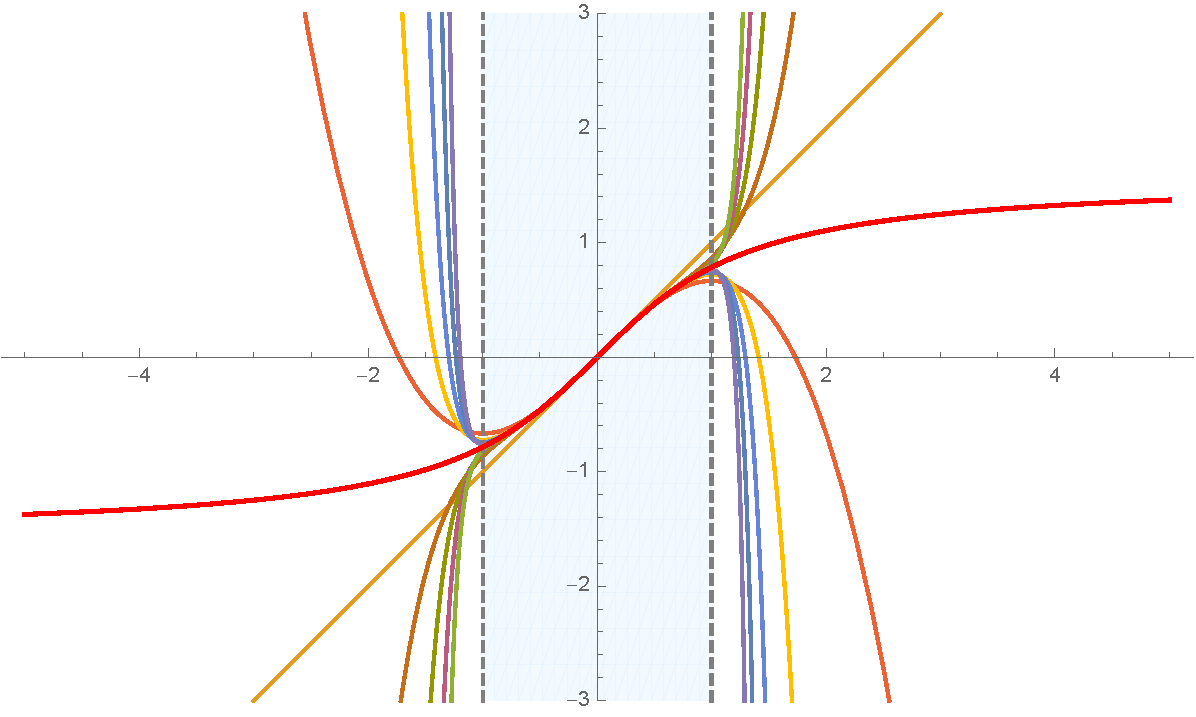
\includegraphics{./images/ch13/arctan-1.pdf}}
	\end{center}

	2、下面换一种方式
	$$(\arctan x)'=\df1{1+x^2}=\df1{x^2}\df1{1+\frac1{x^2}}
	=\df1{x^2}\sum\limits_{n=0}^{\infty}\df{(-1)^n}{x^{2n}}
	=\sum\limits_{n=0}^{\infty}\df{(-1)^n}{x^{2n+2}}, \quad (|x|>1),$$
	当$x>1$时,两边积分
	\begin{align*}
	\arctan x&=\arctan(+\infty)-
	\dint_x^{+\infty}\sum\limits_{n=0}^{\infty}\df{(-1)^n}{t^{2n+2}}\d t\\
	&=\df{\pi}2-\sum\limits_{n=0}^{\infty}{(-1)^n}\dint_x^{+\infty}\df{\d
	t}{t^{2n+2}} =\df{\pi}2-\sum\limits_{n=0}^{\infty}\df{(-1)^{n}}{(2n+1)x^{2n+1}},
	\end{align*}
	以上右侧级数的收敛域为$x\geq 1$;同理,$x<1$时,
	$$\arctan x=-\df{\pi}2
	-\sum\limits_{n=0}^{\infty}\df{(-1)^{n}}{(2n+1)x^{2n+1}},$$
	右侧级数的收敛域为$x\leq -1$。综上
	$${\b\arctan x=\mathrm{sgn}(x)\df{\pi}2-\sum\limits_{n=0}^{\infty}
	\df{(-1)^{n}}{(2n+1)x^{2n+1}},\quad |x|\geq1.}$$

	\begin{center}
		\resizebox{!}{5cm}{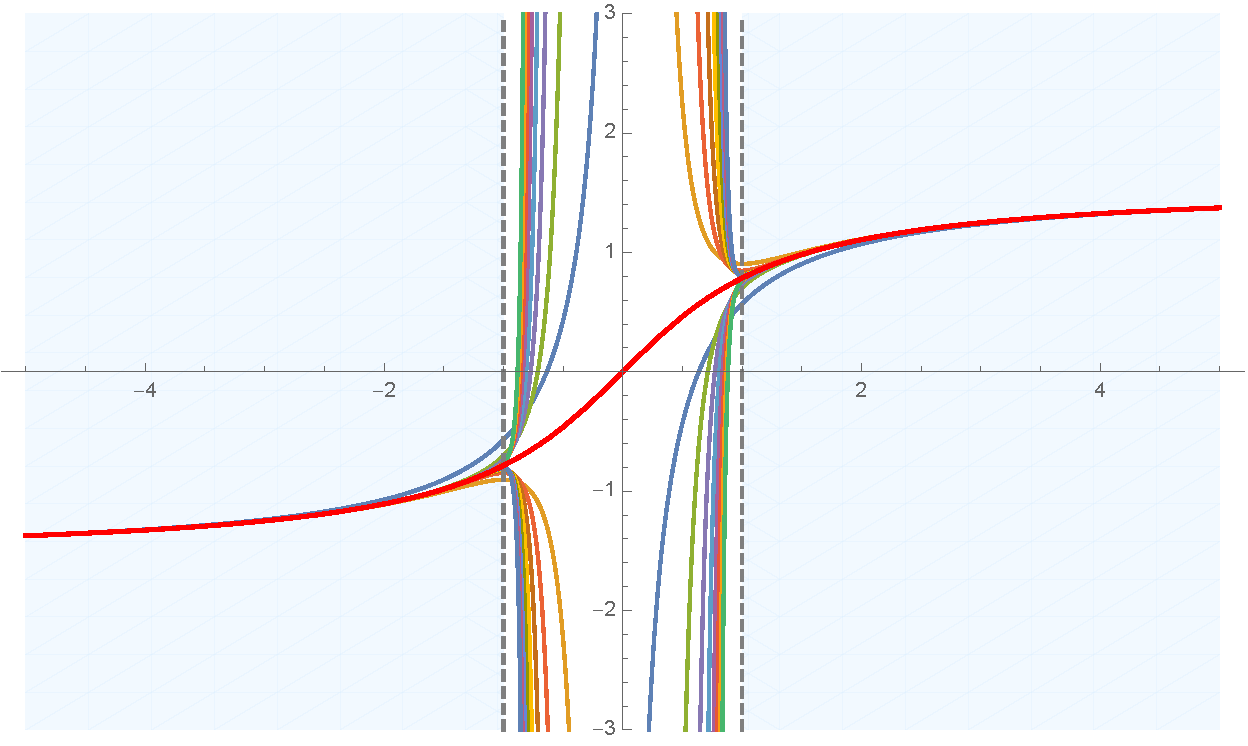
\includegraphics{./images/ch13/arctan-2.pdf}}
	\end{center}

	3、至此我们可以看到,同一个函数$\arctan x$可以由两种不同的展开式,似乎
	与函数的幂级数展开式的唯一性矛盾,真的是这样吗?

	答案是否定的!因为我们得到的第二个展开式并不是幂级数。

	对于$\arctan x$来说,其幂级数展开的“有效”区间(收敛域)只是$[-1,1]$,而
	$\arctan x$在定义区间$(-\infty,+\infty)$内是无穷次可导的,用幂级数展开
	只能表示$\arctan x$的一部分。这个现象说明,
	{\it 幂级数展开的局部性可以有两种理解,一是越靠近展开的位置结果越精确,
	二是这种展开很可能不是对函数的定义域全局有效的}。

	对$\arctan x$来说,以上两个展开式恰好构成了其定义域上完整的表示,使
	我们计算其在任一点处的函数值成为了可能。
% 	也即
% 	$$\arctan x=\left\{\begin{array}{ll}
% 		\sum\limits_{n=0}^{\infty}\df{(-1)^n}{2n+1}x^{2n+1},& |x|\leq 1;\\
% 		\mathrm{sgn}(x)\df{\pi}2-\sum\limits_{n=0}^{\infty}
% 		\df{(-1)^{n}}{(2n+1)x^{2n+1}},&
% 		|x|\geq 1.
% 	\end{array}\right.$$
\end{shaded}

{\bf 例:}将函数$f(x)=\arccos x$展开为$x$的幂级数,写出收敛区间,
并由此给出一个求圆周率$\pi$的公式。

[提示]:
$$(\arccos x)'=-(1-x^2)^{-\frac12}
=-\sum\limits_{n=0}^{\infty}
\left(\begin{array}{c} -\frac12 \\ n \end{array}\right)(-x^2)^n
=-\sum\limits_{n=0}^{\infty}\df{(2n-1)!!}{(2n)!!}x^{2n},
$$
收敛域$(-1,1)$。
故
\begin{align*}
	\arccos x
	&=\df{\pi}2
	-\dint_0^x\sum\limits_{n=0}^{\infty}\df{(2n-1)!!}{(2n)!!}t^{2n}\d t\\
	&=\df{\pi}2-\sum\limits_{n=0}^{\infty}\df{(2n-1)!!}{(2n)!!}\dint_0^xt^{2n}\d
	t\\ 
	&=\df{\pi}2-\sum\limits_{n=0}^{\infty}\df{(2n-1)!!}{(2n)!!(2n+1)}x^{2n+1},
\end{align*}
收敛域$[-1,1]$。

注:以上展开式中的级数当$|x|=1$时,为$\sumn[0]\df{(2n-1)!!}{(2n)!!(2n+1)}$,
判断其收敛需要用到下面的不等式:对任意$k\in\mbb{Z}^+$,$(k-1)(k+1)<k^2$,从而
$$
	\left[\df{(2n-1)!!}{(2n)!!}\right]^2(2n+1)
	=\df{(1\cdot3)(3\cdot5)\ldots[(2n-1)(2n+1)]}
	{(2\cdot2)(4\cdot4)\ldots(2n\cdot2n)}<1,
$$
于是$\df{(2n-1)!!}{(2n)!!}<\df1{\sqrt{2n+1}}$,
进而
$$0<\df{(2n-1)!!}{(2n)!!(2n+1)}<\df1{(2n+1)^{\frac32}},$$
因为$\sumn\df1{(2n+1)^{\frac32}}$收敛,故由比较判别法,所讨论的级数收敛。

\subsection{幂级数的应用}

以下部分具体的例子请参加教材。

\subsubsection{近似计算}

幂级数的应用于Taylor公式的应用本质上是相同的,在进行各种近似计算时,
需要将幂级数截断为多项式来使用。与用Taylor公式进行近似计算略有不同
的是,使用幂级数进行近似计算时,对于余项的估计方式略有不同:Taylor公式
主要是使用Lagrange余项进行误差的估值,而幂级数则主要通过对余项的
适当放缩达到控制误差的目的。

{\bf 例:}计算$\dint_0^{\frac12}\df{\arctan x}x\d x$的近似值,
误差不超过$10^{-3}$。

[解]:$|x|\leq 1$时,\ps{参见12.3.5节的讨论}
$$\arctan x=\sumn[0]\df{(-1)^n}{2n+1}x^{2n+1},$$
从而
$$\df{\arctan x}x=\sumn[0]\df{(-1)^n}{2n+1}x^{2n}.$$
进而
$$\dint_0^x\df{\arctan t}x\d t
=\dint_0^x\sumn[0]\df{(-1)^n}{2n+1}t^{2n}\d t
=\sumn[0]\df{(-1)^n}{2n+1}\dint_0^xt^{2n}\d t
=\sumn[0]\df{(-1)^n}{(2n+1)^2}x^{2n+1}.$$
展开到第$2n+1$项的误差
\begin{align*}
	|r_n|
	&=\left|\sum\limits_{k=n+1}^{\infty}
	\df{(-1)^k}{(2k+1)^2}x^{2k+1}\right|\\
	&=\left|x^{2n+1}\left[\df1{(2n+3)^2}
	-\df1{(2n+5)^2}+\df1{(2n+7)^2}-\ldots\right]\right|\\
	&<\df{|x^{2n+1}|}{(2n+3)^2},
\end{align*}
带入$x=\df12$,令$|r_n|\leq 10^{-3}$,可以推出$n\geq 3$,故所求结果
$$\dint_0^{\frac12}\df{\arctan x}x\d x
\approx \df12-\df1{3^2}\df1{2^3}+\df1{5^2}\df1{2^5}-\df1{7^2}\df1{2^7}
=\df{687539}{1411200}\approx 0.487.$$
\fin 

\begin{shaded}
	{\kaishu 以下两个有趣的例子来自于Stewart微积分2015版}

	{\bf 狭义相对论与Newton力学}
	
	Einstein的狭义相对论给出了物体质量与速度的关系式
	$$m=\df{m_0}{\sqrt{1-v^2/c^2}},$$
	其中$m$表示物体以速度$v$运动时的质量,	$m_0$表示物体静止时的质量,
	$c$为真空中的光速。此外,他将物体的总能量定义为其质量与光速的平方的
	乘积。进而根据该公式,他定义物体的动能(Kinetic Engergy)
	等于其运动和静止状态下所对应的总能量之差
	$$K=mc^2-m_0c^2=m_0c^2
	\left[\left(1-\df{v^2}{c^2}\right)^{-1/2}-1\right].$$
	记$x=-v^2/c^2$,则根据$(1+x)^{-1/2}$的Maclaurin公式
	\begin{align*}
		(1+x)^{-/2}
		&=1-\df12+\df{\left(-\frac12\right)\left(-\frac32\right)}{2!}x^2
		+\df{\left(-\frac12\right)\left(-\frac32\right)\left(-\frac52\right)}{3!}x^3\\
		&=1-\df12x+\df38x^2-\df5{16}x^3+\ldots,
	\end{align*}
	可得
	$$K=m_0c^2\left(\df12\df{v^2}{c^2}+\df38\df{v^4}{c^4}
	+\df5{16}\df{v^6}{c^6}+\ldots\right).$$
	在日常生活中,$v$总是远小于$c$,此时忽略上式中的高阶项,可得近似公式
	$$K\approx \df12m_0v^2.$$
	这恰好就是Newton力学体系之下对动能的定义!
	
	试着考虑一下$v=100$m/s时的误差。记$f(x)=m_0c^2[(1+x)^{-1/2}-1]$,
	则$f''(x)=\frac34m_0c^2(1+x)^{-5/2}$。我们知道$c=3\times 10^8$m/s,
	于是,以上近似对应的误差($x=-v^2/c^2$)
	$$|R_1(x)|\leq\df{3m_0c^2\max\limits_{0<\xi<v}|f''(\xi)|}{4\cdot2!}x^2
	<(4.17\times 10^{-10})m_0.$$
	这个误差看起来确实是很小的。
	
	{\bf 光学}
	\begin{center}
		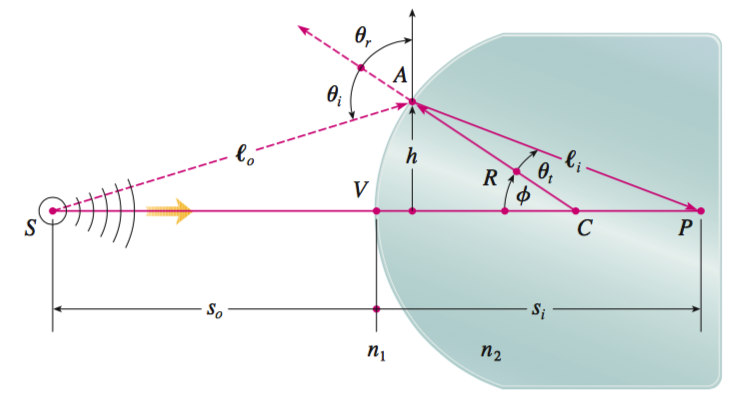
\includegraphics[width=0.8\textwidth]{./images/ch12/refractionSph.png}
	\end{center}
	
	如图,一束光波从$S$出发,经过一个球面(半径为$R$,球心为$C$)上一点$A$,折射到达
	点$P$。
	
	根据Fermat提出的{\kaishu 光路最速原理},光线所经过的路线总是所有路线中耗时最短的一条,
	可以推出如下的公式:
	$$\df{n_1}{l_0}+\df{n_2}{l_i}=\df1R\left(\df{n_2s_i}{l_i}
	-\df{n_1s_0}{l_0}\right),$$
	其中$n_1$和$n_2$分别为折射率,而利用余弦定理,
	$$l_0=\sqrt{R^2+(s_0+R)^2-2R(s_0+R)\cos\phi},$$
	$$l_i=\sqrt{R^2+(s_i+R)^2+2R(s_i+R)\cos\phi}.$$
	注意到前述第一个方程是很难处理的,1841年,Gauss提出,对于很小的$\phi$,
	$\cos\phi\approx 1$,从而将该方程化简为
	$$\df{n_1}{s_0}+\df{n_2}{s_i}=\df{n_2-n_1}R.$$
	这一结果被称为{\kaishu Gauss光学},或者{\kaishu 一阶光学}。
	
	如果考虑$\cos\phi$的跟高阶近似(这时$\phi$相对不那么小了),这可以得到下面这个
	所谓的{\kaishu 三阶光学}公式:
	$$\df{n_1}{s_0}+\df{n_2}{s_i}=\df{n_2-n_1}R
	+h^2\left[\df{n_1}{2s_0}\left(\df1{s_0}+\df1R\right)^2
	+\df{n_2}{2s_i}\left(\df1R-\df1{s_i}\right)^2\right].$$
	
	{\bf 黑体辐射理论}
	
	{\kaishu 黑体}是一个理想化的物体,它能够吸收外来的全部电磁辐射,
	并且不会有任何的反射与透射。随着温度上升,黑体所辐射出来的电磁波
	与光线则称做黑体辐射。是一种理想的物理模型,它表示一种能够吸收所有辐射的系统。
	
	19世纪后期提出的Rayleigh-Jeans定律给出了黑体辐射密度(单位立体角内的辐射率)
	的如下表达式
	$$f(\lambda)=\df{8\pi KT}{\lambda^4},$$
	其中$\lambda$表示辐射的波长(以m为单位),$T$为绝对温度(单位K),
	$k$为Bolzmann常数。这一理论对于长波辐射的计算相当准确,但对于短波
	则存在很大误差(根据实验的结果当$\lambda\to0^+$时,$f(\lambda)\to0$,
	但由以上公式会得出$f(\lambda)\to\infty$),这种现象被称为{\kaishu 紫外灾变}
	(ultraviolet catastrophe)。
	
	1900年,Max Planck给出了更加精确的模型(也称为{\kaishu Planck定律}),
	$$f(\lambda)=\df{8\pi h c\lambda^{-5}}{e^{hc/{\lambda kT}}-1},$$
	其中$h=6.6262\times 10^{-34}$J$\cdot$s,称为Planck常数,$c$为真空下的光速。
	
	\begin{center}
		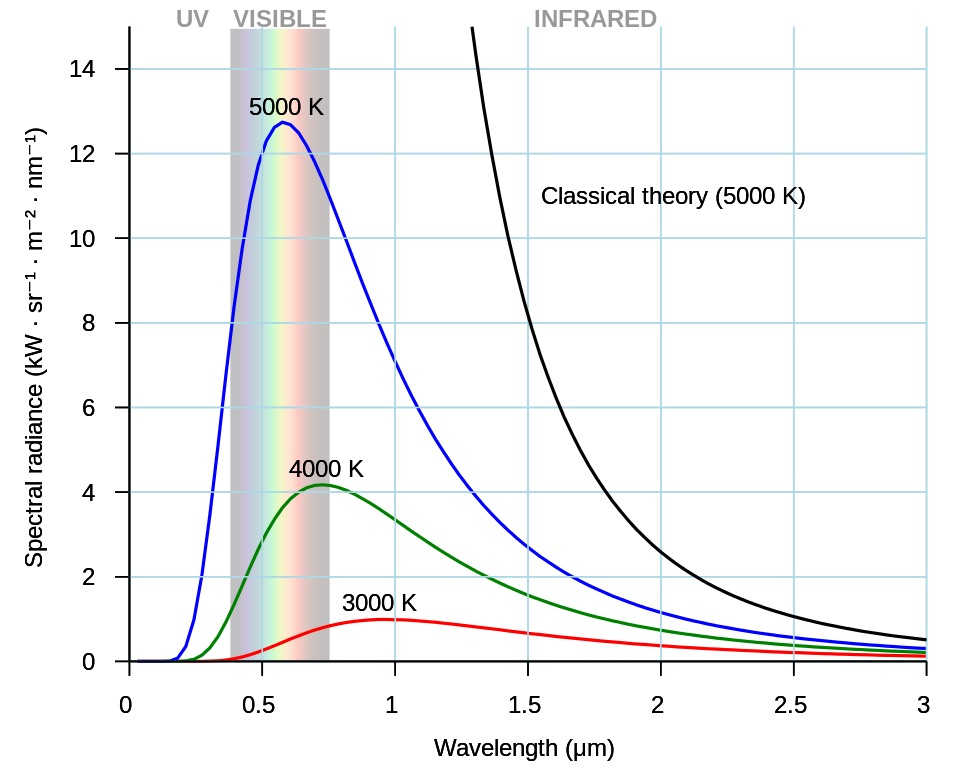
\includegraphics[width=0.6\textwidth]{./images/ch12/blackBody.jpg}
	\end{center}
	
	这一新的定律能够与实验结果很好地吻合($\lambda\to0^+$和$\lambda\to\infty$时,
	均有$f(\lambda\to0)$)。此外,若$\lambda$非常接近于$\infty$(波长很长时),
	令$x=1/\lambda$,则$x\to 0$,此时
	$$e^{hc/{\lambda kT}}-1=e^{hcx/{kT}}-1\approx\df{hcx}{kT},$$
	将右端的近似值带入Planck定律中即得Reyleigh-Jeans定律。从这个意义上说,后者可视为
	对前者的一种近似。
\end{shaded}

\subsubsection{用幂级数求解微分方程}

理论上,幂级数可用于表示任何一个无穷次可导的函数,因此在各种需要求解
具体函数的场合,都可以考虑这样一种间接的思路:首先将待求的函数表示
为一个幂级数,然后设法杰出该幂级数所有的系数,再利用幂级数求和的方法
还原出具体的函数(考虑到并非所有可导的函数都可以表示为初等函数,
很多时候,所得幂级数就是最终要求的函数)。

\subsubsection{Euler公式}

请自行阅读教材。

\bs

\begin{ext}
	{\bf 课后作业}
	\begin{enumerate}
	  \item 求下列函数项级数的收敛域
	  \begin{enumerate}[(1)]
	    \item $\df x{1\cdot 3}+\df{x^2}{2\cdot3^2}+\df{x^3}{3\cdot3^3}
	    +\ldots+\df{x^n}{n\cdot3^n}+\ldots$
	    \item $\sumn\df{(2x+1)^n}n$
	    \item $\sumn(-1)^n\df{x^{2n+1}}{2n}$
	    \item $\sumn\sin\df 1 {3n}\left(\df{3+x}{3-2x}\right)^n$
	  \end{enumerate}
% 	  \hrule
% 	  \item (选作)求级数$\sumn\df1{n^2}$的和。 
% 	  \item 给定两条抛物线$y=nx^2+\df1n,y=(n+1)x^2+\df1{n+1}$,
% 		设其交点的横坐标的绝对值为$a_n$,求:
% 		\begin{enumerate}[(1)]
% 		  \item 两条抛物线所围平面图形的面积$S_n$;
% 		  \item 级数$\sumn\df{S_n}{a_n}$的和。
% 		\end{enumerate}
	  \item 求下列级数的和函数
		\begin{enumerate}[(1)]
		  \item $\sumn(-1)^{n-1}nx^{n-1}$;
		  \item $\df1a+\df{2x}{a^2}+\ldots+\df{nx^{n-1}}{a^n}+\ldots$,其中$a>0$.
		  \item $\sumn[0]\df{x^{2n+1}}{n!}$
		\end{enumerate}
	  \item 已知$f_n(x)\;(n\in\mathbb{Z}^+)$满足
		$$f'_n(x)=f_n(x)+x^{n-1}e^x,$$
		且$f_n(1)=\df en$,求级数$\sumn f_n(x)$的和。
	  \item 将下列函数展开成Maclaurin级数,并求其收敛域
		\begin{enumerate}[(1)]
% 		  \item $f(x)=\arcsin x$
		  \item $f(x)=\df1{x^2-4x+3}$
		  \item $f(x)=\df 1{1+x+x^2}$
		\end{enumerate}
	  \item 将函数$f(x)=\df1{\sqrt{3+2x-x^2}}$展开成$x=1$处的幂级数,并求其收敛域。
	  \item 参考{\kaishu 同济教材第十二章第五节“一、近似计算”}的内容,
	  用幂级数计算下列各数的近似值:
	  \begin{enumerate}[(1)]
	    \item $\sqrt[3]e$,误差不超过$10^{-3}$;
	    \item $\dint_0^{\frac12}\df{\arcsin x}x\d x$的近似值,误差不超过$10^{-3}$。 
	  \end{enumerate}
	\end{enumerate}
\end{ext}

\section{Fourier级数}

\subsection{三角级数与Fourier级数}

从近似的效果来看,幂级数是一种{\it 对无穷次可导函数的局部逼近},这种近似
在条件满足的情况下,可以达到非常高的精度,为精确表示各类函数提供了有效的手段。
然而,无穷次可导并不是任何的函数都具有的性质,并且从逼近的效果来看,并没有达到一种
{\kaishu 整体一致}的近似。例如下图,用幂级数对周期函数$\sin x$作展开

\begin{center}
	\resizebox{!}{5cm}{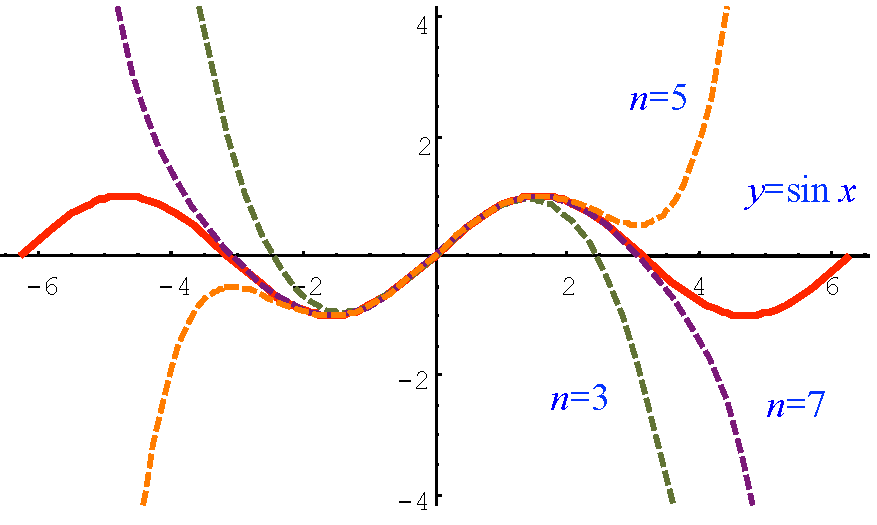
\includegraphics{./images/ch13/sinm.pdf}}
\end{center}

$$\sin x\approx\sum\limits_{k=0}^{n}(-1)^k\df{x^{2k+1}}{(2k+1)!}$$

本节介绍的Fourier级数在这两个方面恰好具有幂级数所不具有的一些性质。当然,
虽然同为函数项级数,但二者的构造特点和性质其实是存在很大差异的。

具体来说,Fourier级数可以说是一种{\it 对周期函数的整体逼近}。这种方法的提出
来自于对周期运动的观察。数学家Daniel Bernoulli提出,任何复杂的振动都可以分
解成一系列简谐振动之和。而Joseph Fourier则进一步推广这一思想,他认为
“任意”函数都可以展开成三角级数。

作为自然界中最基本的一类周期运动(例如弹簧振子、钟摆),
{\it 简谐振动:}可以表示为: $$f(t)=A\sin(\omega t+\varphi)$$
其中:$A$为振幅;$\omega$为角频率;$\varphi$为初相位。
记$x=\omega t,\,a=A\sin\varphi,\,b=A\cos\varphi$, 则
$$g(x)=f(t)=a\cos x+b\sin x.$$

所谓{\bf 三角级数},就是以上这种分解后的简谐振动所构成的无穷和,形如:

$$A_0+\sumn A_n\sin(n\omega t+\varphi_n)$$
或者按照写为如下的形式:
\begin{thx}
	{\bf 三角级数:}
	$${\df{a_0}{2}+\sumn(a_n\cos nx+b_n\sin nx)},$$
	其中$a_0,a_1,b_1,a_2,b_2,\ldots$均为实数。
\end{thx}

{\bf 例:}用三角级数逼近方波的效果

$${f(x)=\df{\pi}{4}\mathrm{sgn}(x),\;(x\in[-\pi,\pi])
\;{\sim\;\sum\limits_{k=1}^n\df{\sin(2k-1)x}{2k-1}}}$$

\begin{center}
	\begin{tabular}{ccc}
		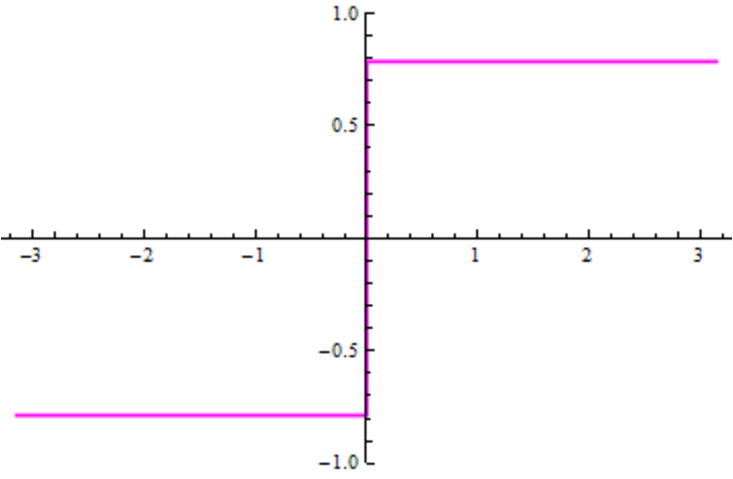
\includegraphics[width=0.3\textwidth]{./images/ch13/fsgn/f0.pdf} &
		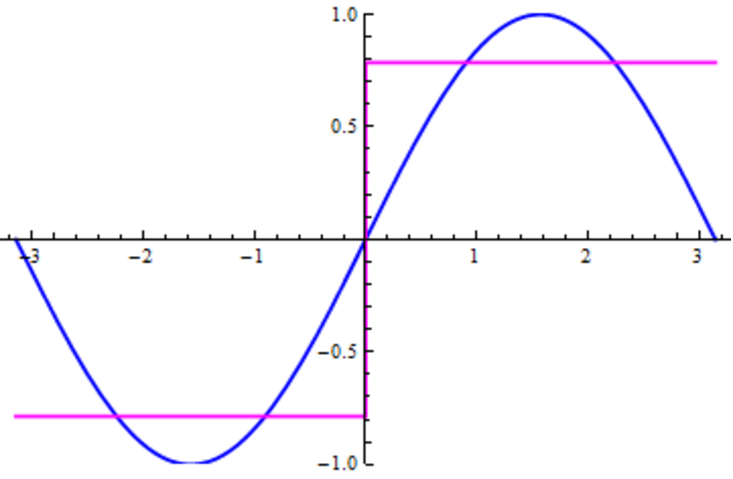
\includegraphics[width=0.3\textwidth]{./images/ch13/fsgn/f1.pdf} &
		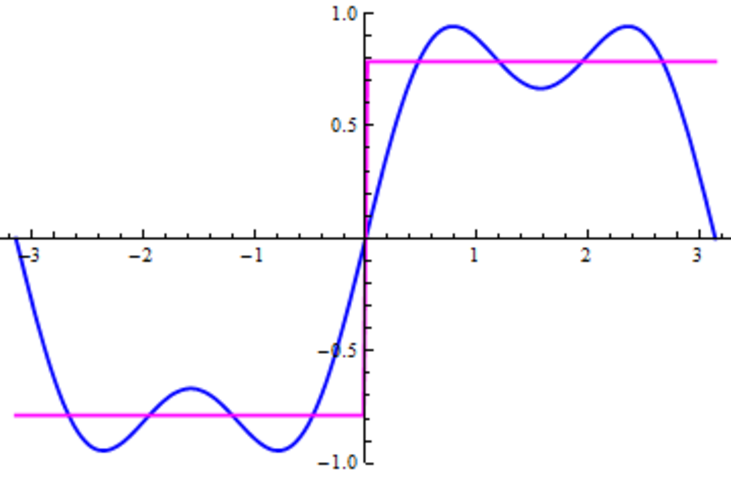
\includegraphics[width=0.3\textwidth]{./images/ch13/fsgn/f2.pdf} \\
		$f(x)=\frac{\pi}4\mathrm{sgn}(x)$ & $n=1$ & $n=2$\\[1em]
		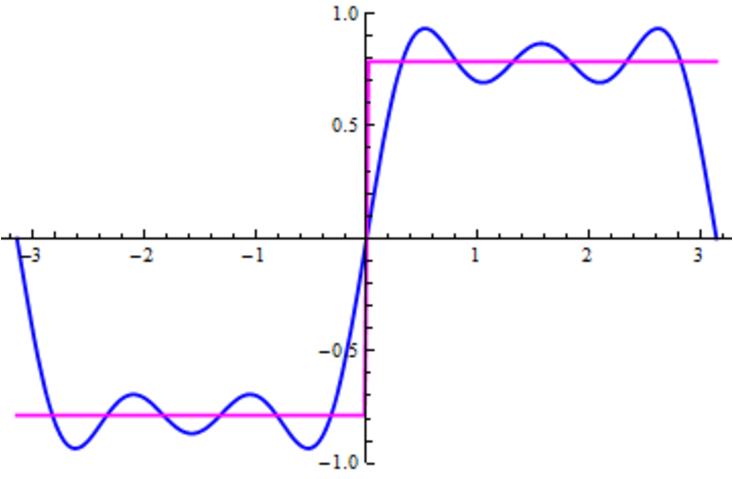
\includegraphics[width=0.3\textwidth]{./images/ch13/fsgn/f3.pdf} &
		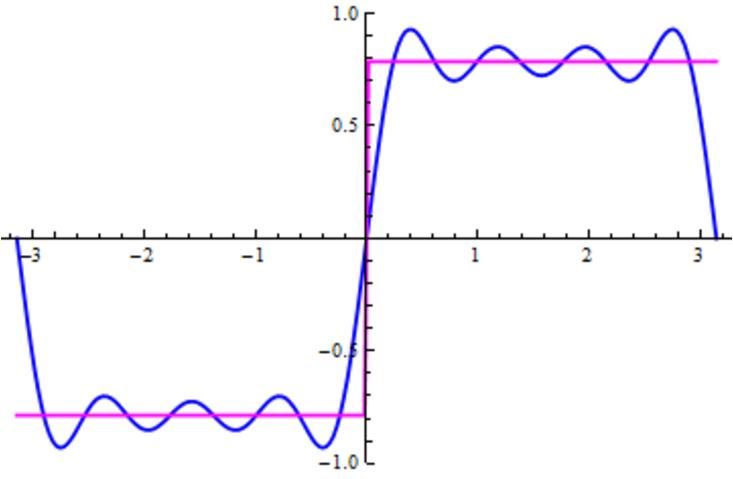
\includegraphics[width=0.3\textwidth]{./images/ch13/fsgn/f4.pdf} &
		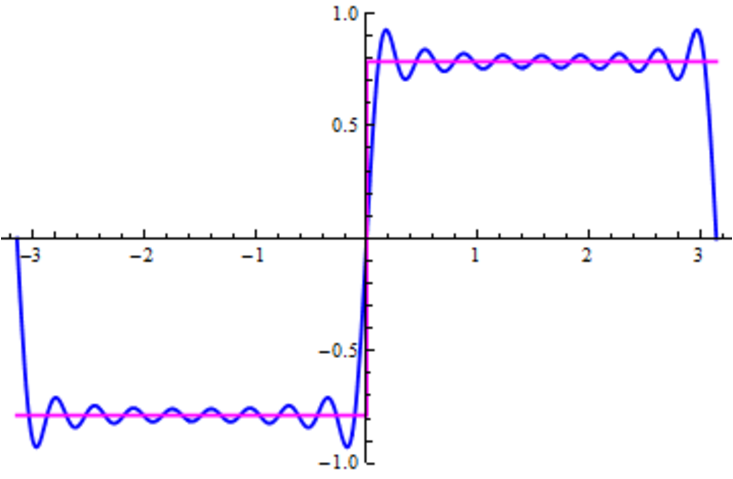
\includegraphics[width=0.3\textwidth]{./images/ch13/fsgn/f5.pdf} \\
		$n=3$ & $n=4$ & $n=5$
	\end{tabular}
% 	\resizebox{!}{4cm}{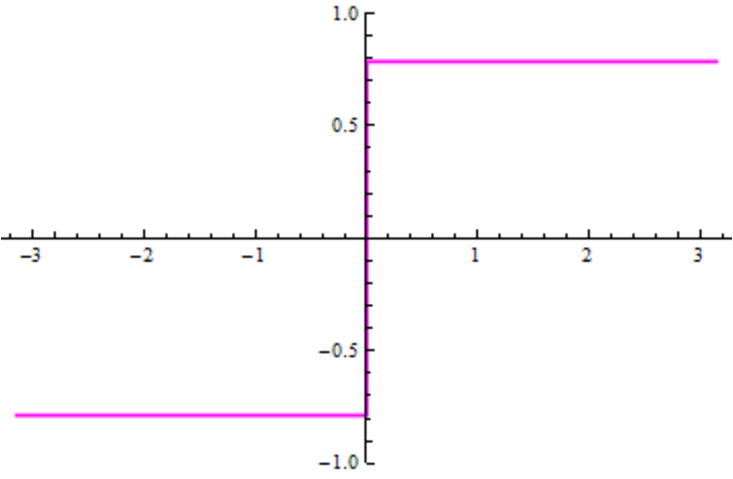
\includegraphics{./images/ch13/fsgn/f0.pdf}}
% 	\quad
% 	\resizebox{!}{4cm}{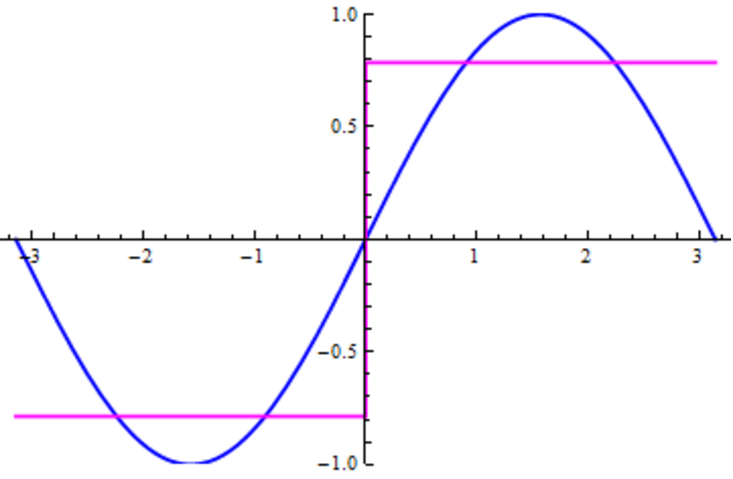
\includegraphics{./images/ch13/fsgn/f1.pdf}}
% 	
% 	\resizebox{!}{4cm}{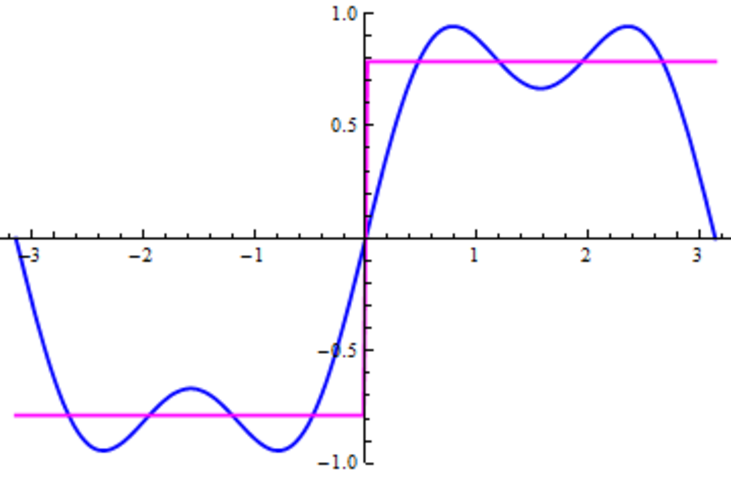
\includegraphics{./images/ch13/fsgn/f2.pdf}}
% 	\quad
% 	\resizebox{!}{4cm}{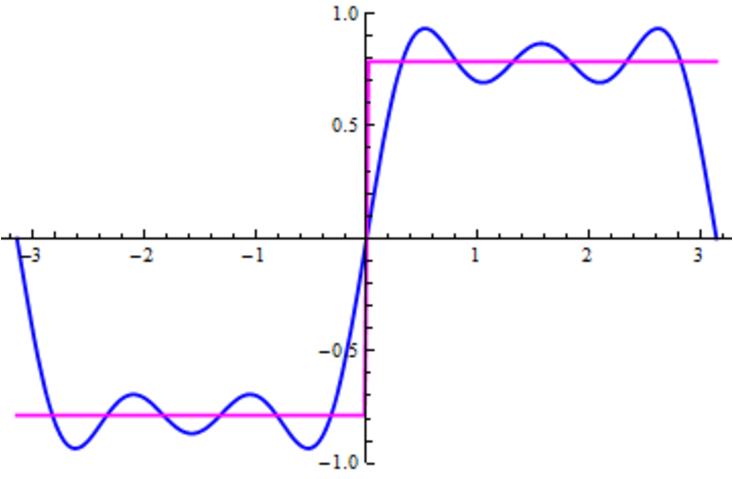
\includegraphics{./images/ch13/fsgn/f3.pdf}}
% 	
% 	\resizebox{!}{4cm}{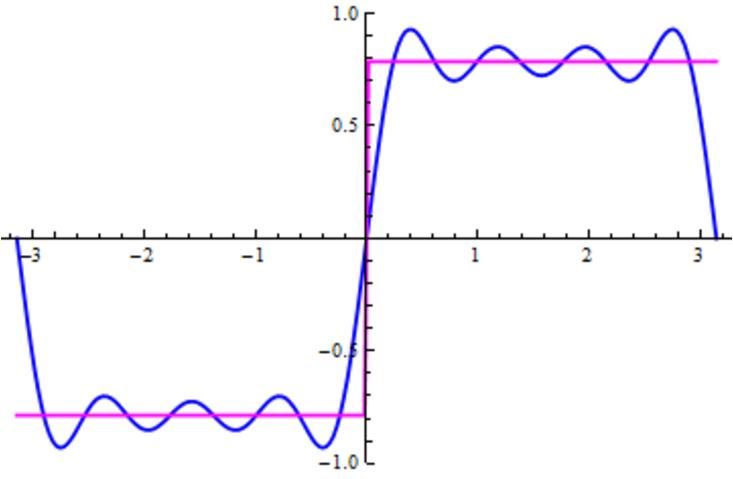
\includegraphics{./images/ch13/fsgn/f4.pdf}}
% 	\quad
% 	\resizebox{!}{4cm}{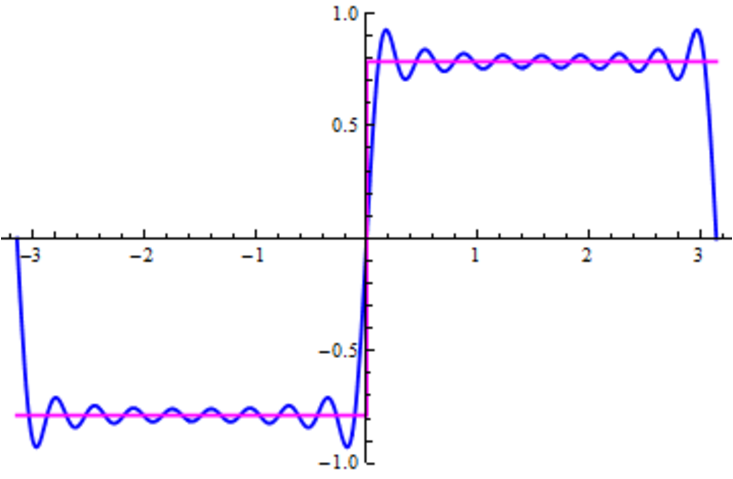
\includegraphics{./images/ch13/fsgn/f5.pdf}}
\end{center}

\begin{shaded}
	{\bf Fourier's Motivation}
	
	以下内容引自Wikipedia关于Fourier Series的条目。
	
	{\it
		The Fourier series is named in honour of \underline{Jean-Baptiste Joseph 
		Fourier} (1768–1830), who made important contributions to the 
		study of \underline{trigonometric series}(三角级数), after preliminary
		investigations by \underline{Leonhard Euler}, 
		\underline{Jean le Rond d'Alembert}, and \underline{Daniel Bernoulli}.
		{\b Fourier introduced the series for the purpose of solving the 
		\underline{heat equation}(热方程) in a metal plate}, publishing his initial
		results in his 1807 Mémoire sur la propagation de la chaleur dans 
		les corps solides (Treatise on the propagation of heat in 
		solid bodies,《热的解析理论》), and publishing his Théorie analytique de 
		la chaleur (Analytical theory of heat) in 1822. The Mémoire 
		introduced Fourier analysis, specifically Fourier series. 
		Through Fourier's research the fact was established that 
		an arbitrary (continuous) function can be represented by 
		a trigonometric series(任意给定的函数均可以表示为一个三角级数). 
		The first announcement of this 
		great discovery was made by Fourier in 1807, before the 
		French Academy. Early ideas of decomposing a periodic 
		function into the sum of simple oscillating functions date 
		back to the 3rd century BC, when ancient astronomers proposed 
		an empiric model of planetary motions, based on deferents and 
		epicycles.

		The heat equation is a partial differential equation(偏微分方程). 
		Prior to Fourier's work, no solution to the heat equation 
		was known in the general case, although particular solutions 
		were known if the heat source behaved in a simple way, in 
		particular, if the heat source was a sine or cosine wave. 
		These simple solutions are now sometimes called eigensolutions. 
		Fourier's idea was to model a complicated heat source as a 
		superposition (or linear combination) of simple sine and 
		cosine waves, and to write the solution as a superposition 
		of the corresponding eigensolutions. This superposition or 
		linear combination is called the Fourier series.
		
		From a modern point of view, Fourier's results are somewhat 
		informal, due to the lack of a precise notion of function and 
		integral in the early nineteenth century. Later, \underline{Peter 
		Gustav Lejeune Dirichlet} and \underline{Bernhard Riemann} expressed Fourier's 
		results with greater precision and formality.
		
		Although the original motivation was to solve the heat equation, 
		it later became obvious that the same techniques could be applied 
		to a wide array of mathematical and physical problems, and 
		especially those involving linear differential equations with 
		constant coefficients, for which the eigensolutions are sinusoids. 
		The Fourier series has many such applications in electrical 
		engineering(电子工程), vibration analysis(振动分析), acoustics(声学), 
		optics(光学), signal processing(信号处理), image processing(图像处理), 
		quantum mechanics(量子力学), econometrics(计量经济学), 
		thin-walled shell theory(?), etc.
	}
	
	下面据说是Fourier最初的工作:
	
	考虑位于平面区域$[0,\pi]\times[0,\pi]$上的金属薄片,已知其上的温度分布$T(x,y)$满足
	{\kaishu 热(传导)方程}
	$$\df{\p^2T}{\p x^2}+\df{\p^2T}{\p y^2}=0,$$
	以及如下的边界条件:
	$$T(x,0)=T(0,y)=T(\pi,y)=0,\quad T(x,\pi)=x,$$
	求$T(x,y)$。
	
	\begin{center}
% 		\resizebox{!}{5cm}{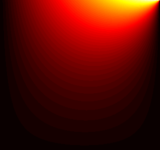
\includegraphics{./images/ch13/Fourier_heat_in_a_plate.pdf}}
% 		\quad
		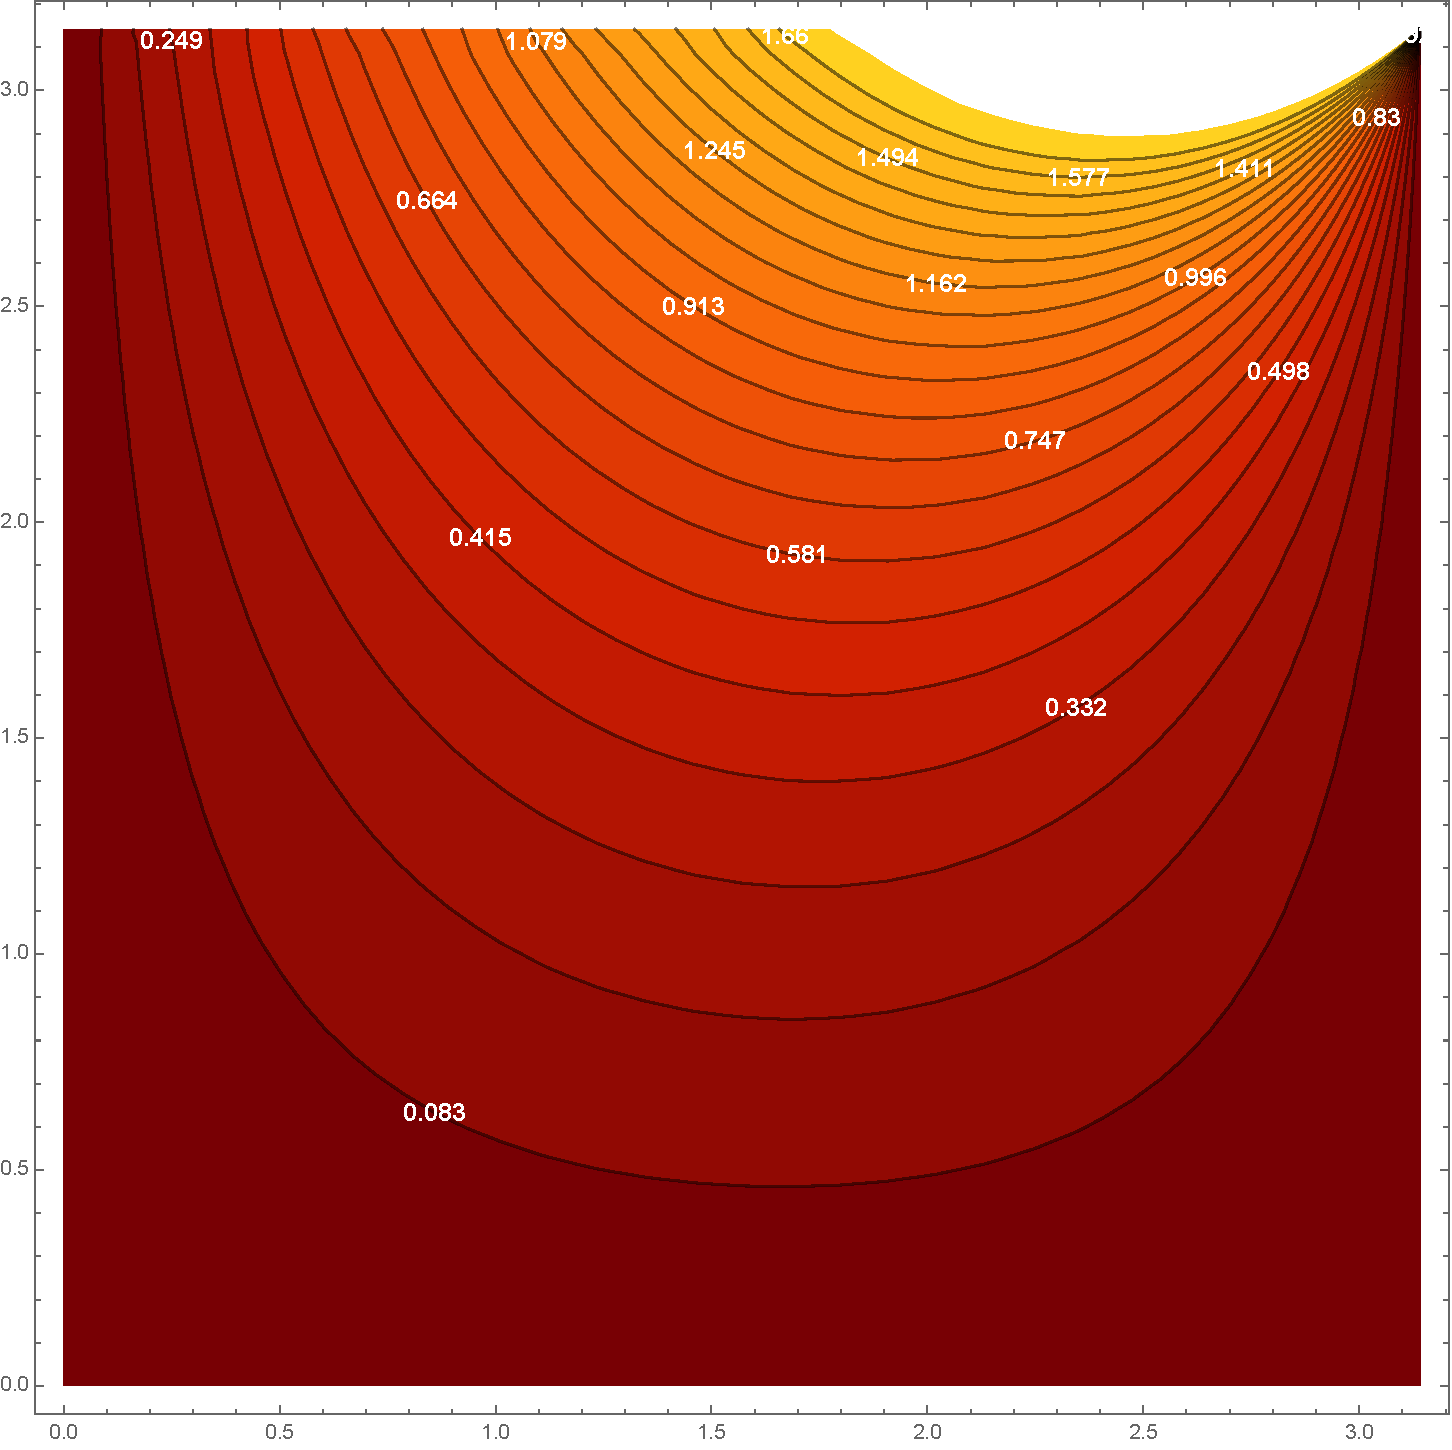
\includegraphics[width=.6\textwidth]{./images/ch12/heatPlane.pdf}
		
		{\it $T(x,y)$的等温线——从红到白,温度逐渐升高}
	\end{center}
	
	注:$T(x,y)$可以理解为处于热平衡状态(金属片上不再发生热传导)时的温度分布。
	这里所考虑的方程只是热方程的一种简单形式,但以下的方法为求解更为
	复杂和一般的问题提供了思路。
	
	Fourier的思路是这样的:很久以来,人们都知道如果以上的最后一个边界条件改为
	$$T(x,\pi)=\sin nx,\;n=1,2,3,\ldots,$$
	其他条件均不变,则热方程存在如下的解(一般称为{\it 本征解})
	$$T(x,y)=\sin nx\df{\sinh ny}{\sinh n\pi}
	=\sin nx\cdot\df{e^{ny}-e^{-ny}}{e^{n\pi}-e^{-n\pi}}.$$
	
	Fourier注意到这样一个事实,给定不同的边界条件,其叠加后产生的温度分布也是可以叠加的。以
	我们这里所考虑的问题为例,也即:给定四个边上的多组边界函数$(a_i(x),b_i(x),c_i(x),
	d_i(x)),(i=1,2,\ldots,n)$,若其对应的温度分布分别为$T_i(x,y),(i=1,2,\ldots,n)$,
	则对于叠加后边界函数$\sum\limits_{i=1}^n(a_i(x),b_i(x),c_i(x),d_i(x))$,其相应的
	温度分布就是所有对应温度分布的叠加,也即:$\sum\limits_{i=1}^nT_i(x,y)$。
	
	因此,Fourier想到,如果$x$可以表示为$\{\sin nx|n=1,2,3,\ldots\}$的叠加
	(线性组合)形式,那么利用同样的线性组合,由这些边界函数对应的本征解就可以叠加构造
	出$x$对应的问题的解。
	
	最终,Fourier利用如下的三角级数(如何得到类似这样的三角级数,正是我们需要在高等数学课程
	中学习的)
	$$x=2\sumn\df{(-1)^{n+1}}{n}\sin{nx},\quad x\in[0,\pi],$$
	得到了最终的温度分布
	$$T(x,y)=2\sumn\df{(-1)^{n+1}}{n}\sin{nx}
	\cdot\df{e^{ny}-e^{-ny}}{e^{n\pi}-e^{-n\pi}}.$$
	
	\begin{center}
		\begin{tabular}{ccc}
			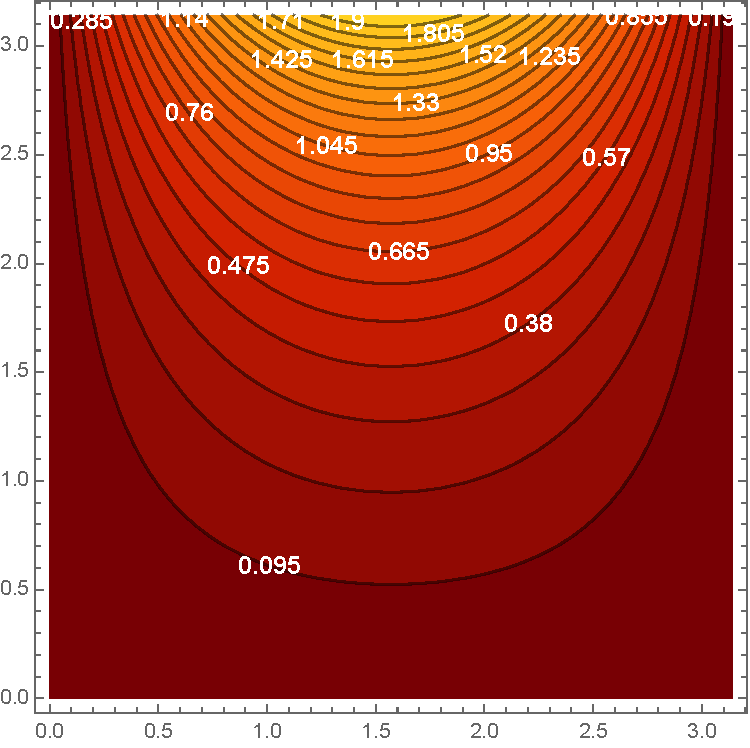
\includegraphics[width=0.3\textwidth]{./images/ch12/n1.pdf} &
			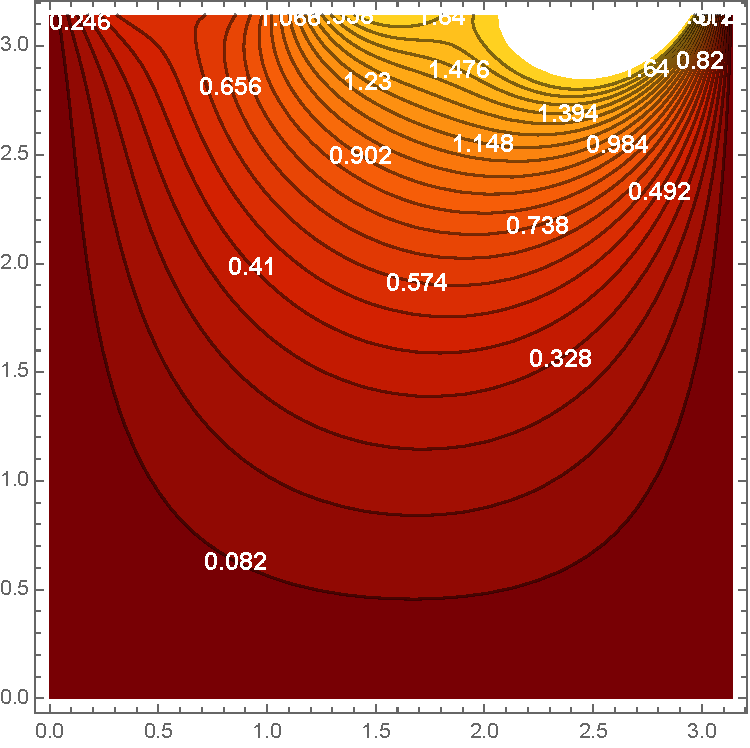
\includegraphics[width=0.3\textwidth]{./images/ch12/n5.pdf} &
			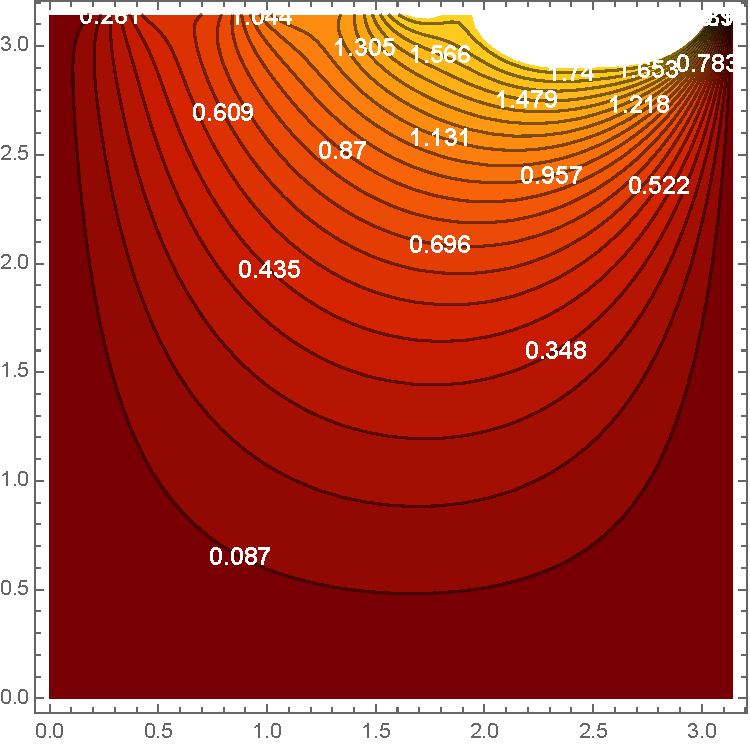
\includegraphics[width=0.3\textwidth]{./images/ch12/n10.pdf}\\
			$n=1$ & $n=5$ & $n=10$\\[1em]
			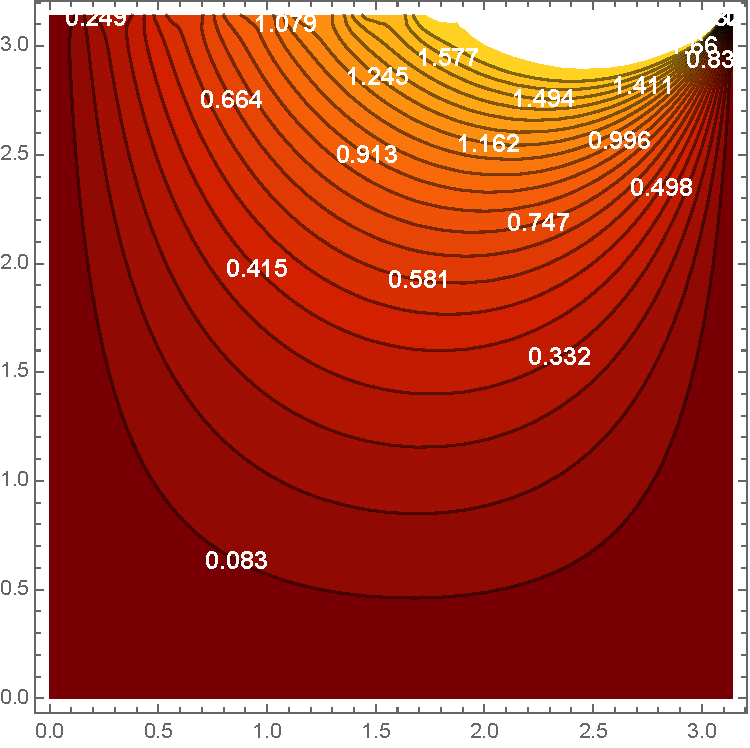
\includegraphics[width=0.3\textwidth]{./images/ch12/n20.pdf} &
			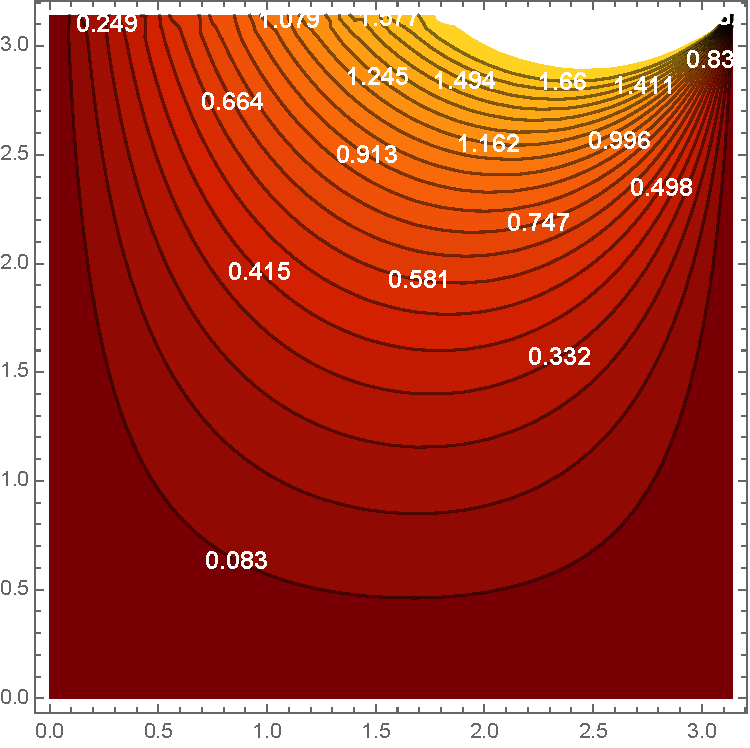
\includegraphics[width=0.3\textwidth]{./images/ch12/n30.pdf} &
			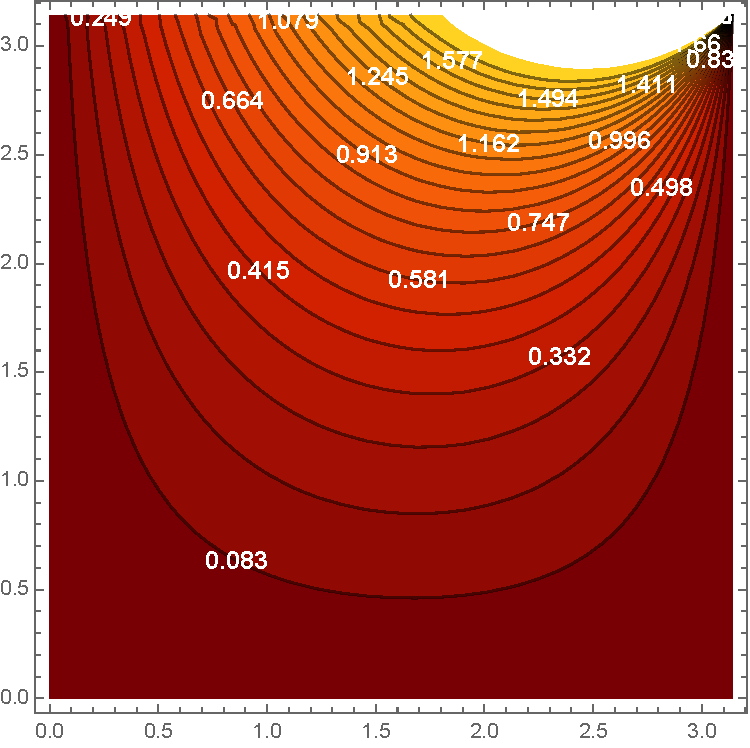
\includegraphics[width=0.3\textwidth]{./images/ch12/n50.pdf}\\
			$n=20$ & $n=30$ & $n=50$
		\end{tabular}
	\end{center}
\end{shaded}
 
之所以能够对任意给定的函数进行三角级数展开,关键的原因在于三角函数列所具有的
{\kaishu 正交性}:

\begin{thx}
	{\bf 三角函数序列$A=\{\cos kx,\sin kx|k=1,2,\ldots\}$的正交性}:
	任意$f(x),g(x)\in A$,
	$$\dint_{-\pi}^{\pi}f(x)g(x)dx=\left\{\begin{array}{ll}
	0,\;& f(x)\ne g(x)\\ \pi\;& f(x)=g(x)
	\end{array}\right.$$
\end{thx}

{\bf 注:}将常值函数$1$加入$A$中,不改变其正交性,只是$1$不满足
平方积分等于$\pi$(而是等于$2\pi$)。因此,在Fourier展开式中,
与$1$对应的系数$a_0$需要除以$2$。

\begin{thx}
	若函数$f(x)$可展成如下三角级数
	$$\df{a_0}{2}+\sumn(a_n\cos nx+b_n\sin nx),$$
	且该三角级数可逐项积分, 则
	$$\left\{\begin{array}{ll}
	a_n=\df1{\pi}\dint_{-\pi}^{\pi}f(x)\cos nx\d x,\;& n=0,1,2,\ldots\\[5pt]
	b_n=\df1{\pi}\dint_{-\pi}^{\pi}f(x)\sin nx\d x,\;& n=1,2,\ldots
	\end{array}\right.$$
	以上所得$a_n,b_n$称为函数$f(x)$的{\bf Fourier系数},由其所
	构成的三角级数称为$f(x)$的{\bf Fourier级数}。
\end{thx}

\begin{shaded}
	{\bf 利用正交函数列构造函数项级数}
	
	如果能够找到与$A$类似的一个正交函数序列,则可以利用以上定理的
	思想来构造类似Fourier级数的函数项级数。
	
	例如:$B=\{\xi_n(x)\}$,其中
	$\xi_n(x),\;n=0,1,2,\ldots$均为以$2$为周期的函数,且在$x\in[0,2]$上,
	$$
		\left\{\begin{array}{rl}
			\xi_0(x)&=1\\
			\xi_1(x)&=(-1)^{[x]}\\
			\xi_2(x)&=(-1)^{[2x]}\\
			\xi_3(x)&=(-1)^{[4x]}\\
			\ldots&\ldots\\
			\xi_n(x)&=(-1)^{[2^nx]}\\
			\ldots&\ldots
		\end{array}\right.
	$$
	其中$[x]$表示下取整函数,也即不大于$x$的最大的整数。
	
	\begin{center}
		\begin{tabular}{cc}
			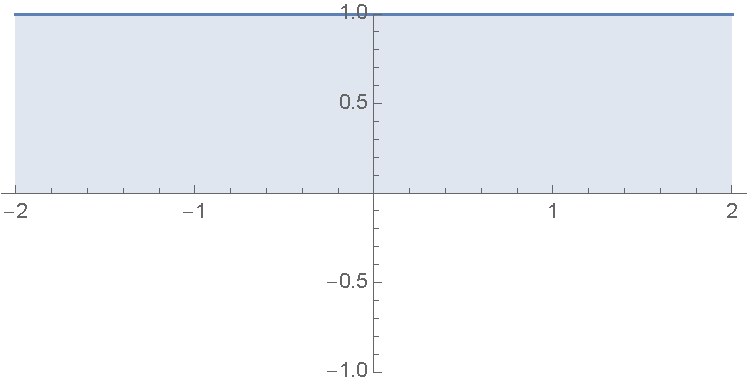
\includegraphics[width=0.4\textwidth]{./images/ch12/xi0.pdf}
			& 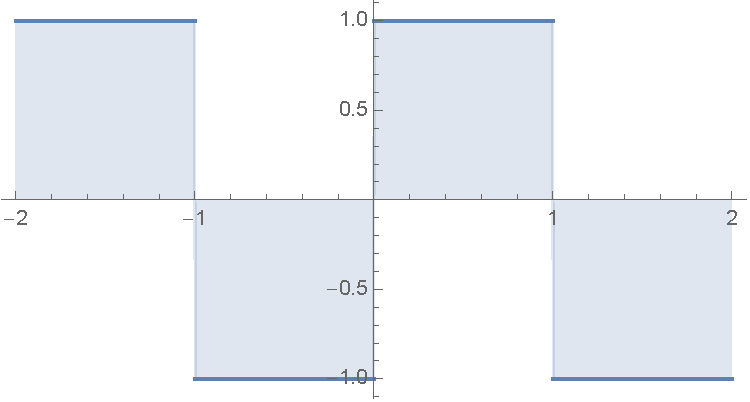
\includegraphics[width=0.4\textwidth]{./images/ch12/xi1.pdf}\\
			$y=\xi_0(x)$ & $y=\xi_1(x)$\\[1em] 
			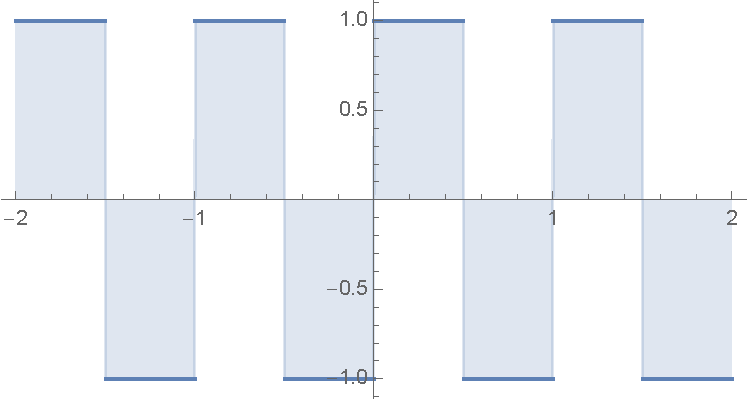
\includegraphics[width=0.4\textwidth]{./images/ch12/xi2.pdf}
			& 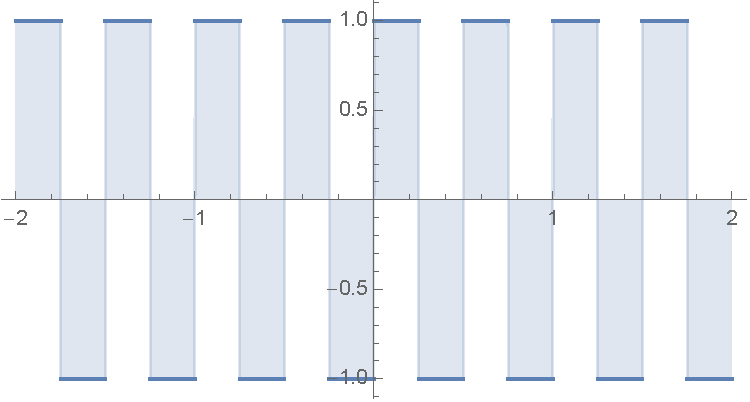
\includegraphics[width=0.4\textwidth]{./images/ch12/xi3.pdf}\\
			$y=\xi_2(x)$ & $y=\xi_3(x)$ 
		\end{tabular}
	\end{center}
	
	可以证明任意$f,g\in B$,均满足:
	$$\dint_0^{2}f(x)g(x)\d x=
	\left\{\begin{array}{ll}
		0,& f\ne g\\ 2,& f=g
	\end{array}\right.$$
	
	参考Fourier级数的有关定理,给以类似地给出如下结论:
	
	\begin{tcolorbox}
		{\bf 定理:}对任意以$2$为周期的函数$f(x)$,若其可以表示为
		$$f(x)\sim\sum\limits_{n=0}^{\infty}u_n\xi_n(x),$$
		且右端级数可以逐项积分,则
		$$
		u_n=\df12\dint_0^2f(x)\xi_n(x)\d x,\;n=0,1,2,\ldots.
		$$
	\end{tcolorbox}
\end{shaded}

{\bf 例:}已知$f(x)=\left\{\begin{array}{ll}
	x,& x\in[-\pi,\pi),\\ f(x+2\pi)& \mbox{其他}
\end{array}\right.$,求其对应的Fourier级数。

[解]:对$n=0,1,2,\ldots$,
$$a_n=\df1{\pi}\dint_{-\pi}^{\pi}x\cos nx\d x=0.$$
对$n=1,2,\ldots$,
\begin{align*}
	b_n&=\df1{\pi}\dint_{-\pi}^{\pi}x\sin nx\d x
	=-\df1{n\pi}\dint_{-\pi}^{\pi}x\d\cos nx\\
	&=-\df1{n\pi}\left[x\cos nx|_{-\pi}^{\pi}
	-\dint_{-\pi}^{\pi}\cos nx\d x\right]=2\df{(-1)^{n+1}}n
\end{align*}
综上,所求Fourier级数为
$$2\sumn\df{(-1)^{n+1}}n\sin nx.$$
\fin

{\bf 例:}$f(x)$以$2\pi$为周期,且在$[-\pi,\pi)$内$f(x)=\df{\pi}{4}\mathrm{sgn}(x)$,
求其Fourier级数。

\begin{thx}
	{\bf Fourier级数的性质}
	\begin{enumerate}%[(1)]
% 	  \setlength{\itemindent}{1cm}
	  \item $[-\pi,\pi]$上的奇函数的Fourier级数只含有正弦项, 称为{\bf 正弦级数}
	  \item $[-\pi,\pi]$上的偶函数的Fourier级数只含有余弦项, 称为{\bf 余弦级数}
	  \item {\kaishu 周期函数积分的平移不变性:}计算以$2\pi$为周期的函数的Fourier级数,
	  积分区间选择任意一个长度为$2\pi$的连续区间即可,也即:任取常数
	  $x_0\in\mathbb{R}$,均有
	  	$$\left\{\begin{array}{ll}
			a_n=\df1{\pi}\dint_{x_0}^{x_0+2\pi}f(x)\cos nx\d x,\;& n=0,1,2,\ldots\\[5pt]
			b_n=\df1{\pi}\dint_{x_0}^{x_0+2\pi}f(x)\sin nx\d x,\;& n=1,2,\ldots
	  	\end{array}\right.$$
	  \item {\bf 只在有限点处取值不同的函数,Fourier级数相同},因为改变函数在有限点
	  处的值,其定积分不变。
	  \item Fourier展开具有{\it 线性性},也即:$f(x)+g(x)$的Fourier系数等于$f(x)$和
	  $g(x)$的Fourier系数的和
	\end{enumerate}
\end{thx}

{\bf 例:}已知$f(x)=\left\{\begin{array}{ll}
	e^x,& x\in[0,2\pi),\\ f(x+2\pi)& \mbox{其他}
\end{array}\right.$,求其对应的Fourier级数。

[提示]:根据$f(x)$的特征,应考虑使用以上注(3)中的公式,也即
$$a_n=\df1{\pi}\dint_{0}^{2\pi}e^x\cos nx\d x,\; n=0,1,2,\ldots,$$
$$b_n=\df1{\pi}\dint_{0}^{2\pi}e^x\sin nx\d x,\; n=1,2,\ldots.$$
如果使用常见的公式形式,则应该为
$$a_n=\df1{\pi}\left[\dint_{-\pi}^{0}e^{x+2\pi}\cos nx\d x+
\dint_{0}^{\pi}e^x\cos nx\d x\right],\; n=0,1,2,\ldots,$$
$$b_n=\df1{\pi}\left[\dint_{-\pi}^{0}e^{x+2\pi}\sin nx\d x+
\dint_{0}^{\pi}e^x\sin nx\d x\right],\; n=1,2,\ldots.$$

{\bf 例:}将下列函数展成Fourier级数
\begin{enumerate}[(1)]
  \setlength{\itemindent}{1cm}
  \item $f(x)=1+3\sin x+4\cos 3x-9\sin 2x$
  \item $f(x)=\sin^4x$
\end{enumerate}

[提示]:(2)利用半角/倍角公式降低幂次
\begin{align*}
	\sin^4x&=\left(\df{1-\cos2x}2\right)^2
	=\df14\left(1-2\cos2x+\cos^22x\right)\\
	&=\df14\left(1-2\cos2x+\df{1+\cos4x}{2}\right)\\
	&=\df38-\df12\cos2x+\df18\cos4x
\end{align*}
即为所求。

{\bf 注:}{\b 以$2\pi$为周期的一次三角多项式的Fourier级数是其自身}

\subsection{Fourier级数的收敛性}

Fourier级数的敛散性是一个相当复杂的问题,这里仅给出与之相关的结论,不予证明:

\begin{thx}
	{\bf Dirichlet收敛条件:}$f(x)$以$2\pi$为周期, 在$[-\pi,\pi]$上其
	仅有有限多个第一类间断点和有限多个极值点,则$f(x)$的Fourier级数处处收敛,
	 其和函数
	$$S(x) =\df{f(x+0)+f(x-0)}{2}.$$
\end{thx}

根据定理条件,可知$f(x)$不可能有第二类间断点,故以上结论可以表述为:
$S(x)$在$f(x)$的连续点处收敛于$f(x)$,在$f(x)$的不连续点处收敛于其左右极限的中点。

{\bf 例:}$f(x)=\sin\df1x$在原点的的任意邻域内均有无穷多个极值点,不满足该条件,因此
其Fourier级数在原点处不收敛。

\begin{center}
	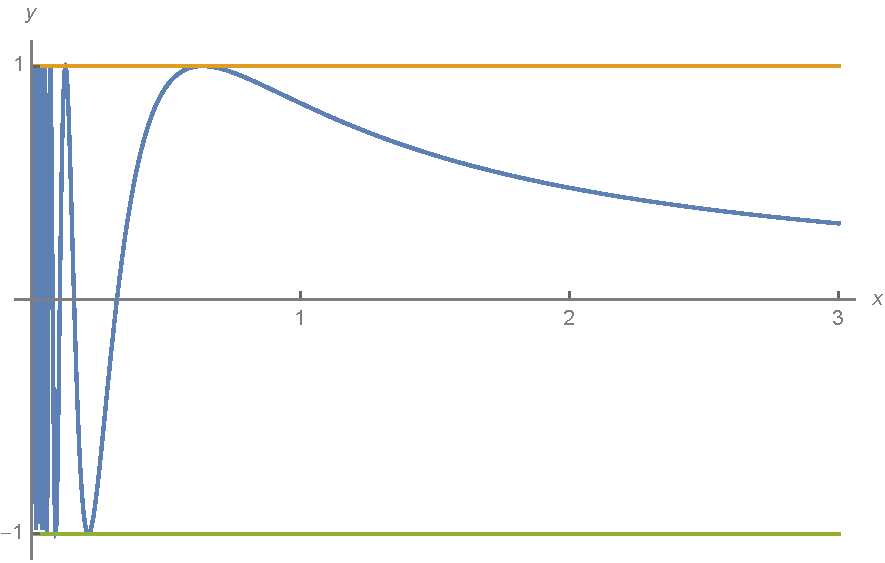
\includegraphics[width=0.5\textwidth]{./images/ch12/sin1x.pdf}
\end{center}

显然,将函数展开成Fourier级数的条件比将其展开成幂级数的条件要低很多。

{\bf 例:}判断正误
\begin{enumerate}[(1)]
  \setlength{\itemindent}{1cm}
  \item 函数$f(x)$连续,在$[-\pi,\pi]$上满足Dirichlet条件且为奇函数,则$f(x)$
  的Fourier级数在$0,\pm\pi$处必收敛于$0$\quad  (\;{$\surd$}\;) 
  \item $f(x)=x^2\,(x\in[-\pi,\pi])$的Fourier级数在$2\pi$处收敛于$4\pi^2$
    \quad(\;{$\times$}\;) 
  \item 以$2\pi$为周期的函数$f(x)=\df x{2\pi}\,(x\in[0,2\pi])$,其Fourier
  级数的和函数为$S(x)$,则$S(0)=f(0)=0$ 
  \quad (\;{$\times$}\;)
  \item 函数$f(x)=x^2\,(x\in[-\pi,\pi])$以$2\pi$为周期,则 
  \begin{itemize}
    \item $\df 1{\pi}\dint_{-\pi}^{\pi}f(x)\sin kxdx=\df
    1{\pi}\dint_{0}^{2\pi}f(x)\sin kxdx$\quad (\;{$\surd$}\;) 
    \item $\df 1{\pi}\dint_{-\pi}^{\pi}x^2\sin kxdx=\df
    1{\pi}\dint_{0}^{2\pi}x^2\sin kxdx$\quad (\;{$\times$}\;) 
  \end{itemize}
  \item 以$2\pi$为周期的函数$f(x)=x^2\,(x\in[-\pi,\pi])$和$g(x)=x^2\,(x\in[0,2\pi])$的
  Fourier级数相同\quad (\;{$\times$}\;)
\end{enumerate}

{\bf 例:}试写出函数
$$f(x)=\left\{\begin{array}{rl}
	-\df{\pi}{4},\; & -\pi\leq x<0\\[8pt]
	\df{\pi}{4},\; & 0\leq x<\pi
\end{array}\right.$$
的Fourier级数的和函数。

[解]:
$${S(x)=\left\{\begin{array}{ll}
	-\pi/4,\;& -\pi<x<0\\
	\pi/4,\;& 0<x<\pi\\
	0,\; & x=0,\pm\pi
\end{array}\right.}$$
\fin

{\bf 例:}设周期函数$f(x)$在一个周期内的表达式为
$$f(x)=\left\{\begin{array}{ll}
	-1,\;& -\pi<x\leq 0\\
	1+x^2,\; & 0<x\leq\pi
\end{array}\right.$$
写出该函数在$[-\pi,\pi]$上的和函数$S(x)$,并求
$S(5\pi/2),S(7\pi/2),S(7\pi)$和$S(2008\pi)$的值。

有时可以利用Fourier级数求一些特殊级数的和:

{\bf 例:}由
$$\df{\pi}4=\sum\limits_{m=1}^{\infty}
\df{\sin(2m-1)x}{2m-1},\;0<x<\pi,$$
 令$x=\pi/2$, 可得
$$\df{\pi}4=1-\df 13+\df 15-\df 17+\ldots
+(-1)^{m-1}\df 1{2m-1}+\ldots$$

{\bf 例:}设$f(x)=|x|\;(-\pi\leq x\leq \pi)$的Fourier级数,并由此
证明:
$$\df{\pi^2}{6}=1+\df 1{2^2}+\df 1{3^2}+\ldots+\df 1{n^2}+\ldots$$

[提示]:
$$f(x)\sim\df{\pi}2-\df 4{\pi}\sum\limits_{m=1}^{\infty} 
\df{\cos(2m-1)x}{(2m-1)^2},\;-\pi\leq x\leq \pi$$
\begin{center}
	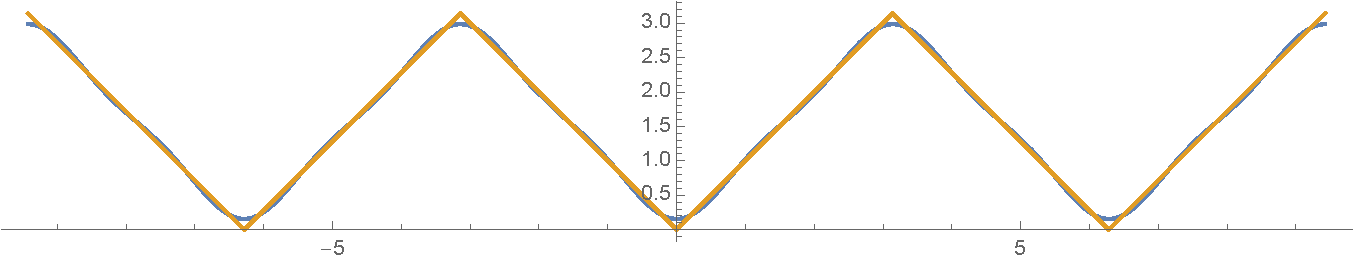
\includegraphics[width=0.8\textwidth]{./images/ch12/xExp3.pdf}
\end{center}

{\bf 例:}设周期函数$f(x)$在一个周期内的表达式为
$$f(x)=e^x\;(x\in[0,2\pi]),$$
试将其展成Fourier级数,并求下列数值级数的和:
$$\sum\limits_{n=1}^{\infty}\df1{1+n^2}$$

[提示]:
$$f(x)\sim\df{e^{2\pi}-1}{\pi}\left[1+
\sumn\df{\cos nx-n\sin nx}{n^2+1}\right]$$
\begin{center}
	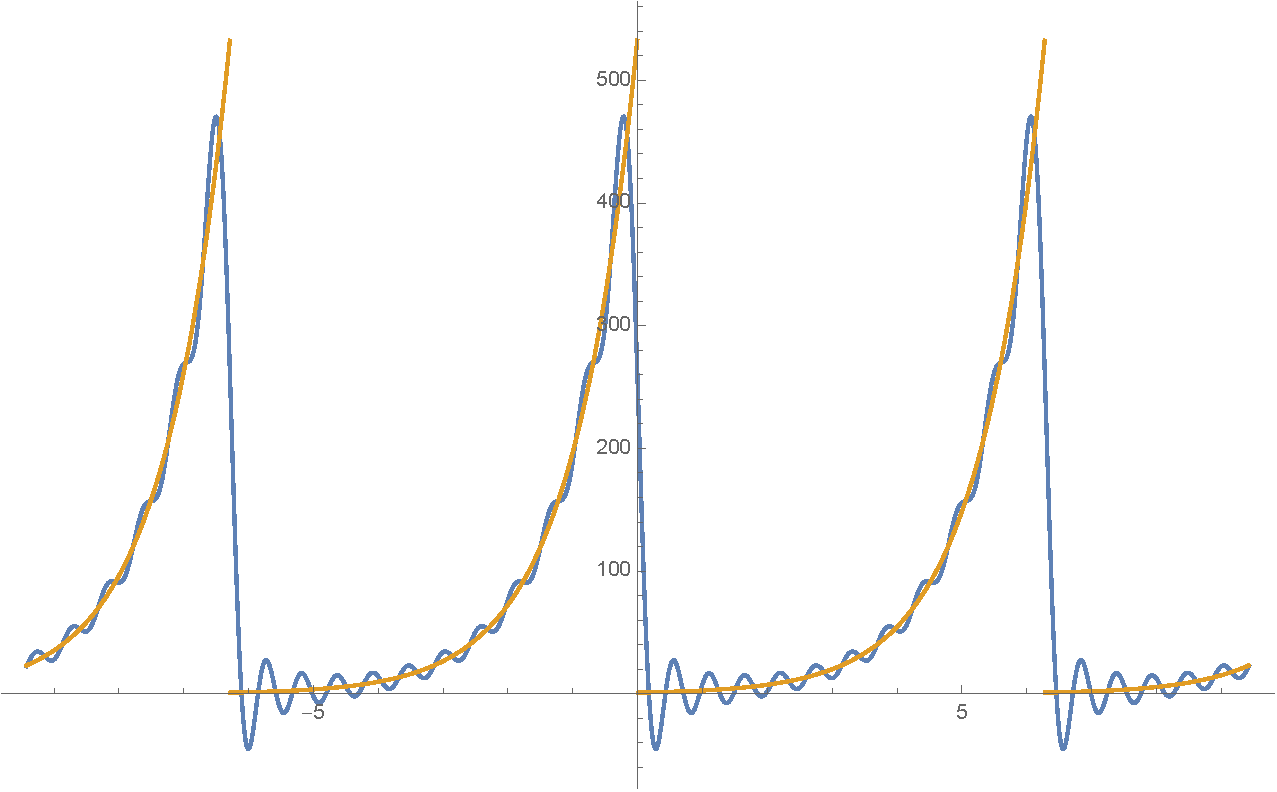
\includegraphics[width=0.6\textwidth]{./images/ch12/expX11.pdf}
\end{center}

Fourier展开给出了求函数的三角级数的方法,但是它需要满足一个基本的条件:
$f(x)$以$2\pi$为周期。

在现实问题中,很多函数并不是周期函数,即使是周期函数,也未必一定以$2\pi$
为周期。针对这样的函数,可以通过对函数(定义区间)的延拓或放缩,使之满足Fourier
展开的条件,然后间接地求得其对应的三角级数。

\subsection{函数的延拓及其Fourier展开}

\subsubsection{周期延拓}

若$f(x)$为定义在$[-\pi,\pi)$上的函数,满足Dirichlet条件。严格来说,为了
对其进行Fourier展开,需要将其视为某个周期函数$F(x)$的一部分,$F(x)$在
$[-\pi,\pi)$上定义与$f(x)$完全相同。这样一来,$F(x)$对应的Fourier级数
也就是$f(x)$的三角级数展开。

\subsubsection{奇(偶)延拓}

考虑定义在$(0,\pi)$上的函数$f(x)$,且在其上满足Dirichlet条件。为了对其进行
Fourier展开,只需为其补充$[-\pi,0]$上的定义,再利用周期延拓构造一个
以$2\pi$在为周期的函数$F(x)$。最后,将$F(x)$作Fourier展开,
其中$(0,\pi)$上的部分即为$f(x)$的三角级数展开。

在补充$[-\pi,0]$上的函数定义时,我们有许多的选择,理论上讲,任意在$[-\pi,0]$
满足Dirichlet条件的函数都是可能的选择。

在前面关于Fourier级数的讨论中我们曾提到,若给定的函数为奇(偶)函数,则
其Fourier级数中只含正(余)弦项,对应的级数可以称为正(余)弦级数。在接下来
的讨论中,我们将着重讨论一下展开后的三角级数分别为正弦和余弦级数的情形,
对应的延拓方式分别称为奇延拓和偶延拓。

具体来说,

\begin{thx}
	{\bf 奇(偶)延拓后的Fourier展开:}设$f(x)$在$(0,\pi)$上满足Dirichlet条件,令
	$$F(x)=\left\{\begin{array}{ll}
	  	f(x),\;& x\in(0,\pi)\\
	  	0,\;& x=0,-\pi\\
	  	\pm f(-x),\;& x\in(-\pi,0)
	  \end{array}\right.$$
	且
	  $$F(x+2\pi)=F(x)\;(-\infty<x<\infty).$$
	这样一来,$F(x)$就是满足Dirichlet条件的偶(奇)周期函数,其Fourier级数为
	余(正)弦级数,其中在$(0,\pi)$内的部分即为$f(x)$对应的余(正)弦级数。
\end{thx}

{\bf 例:}设函数$f(x)=x+1\,(x\in(0,\pi))$,试将其分别展开为正弦和余弦级数。

\begin{center}
	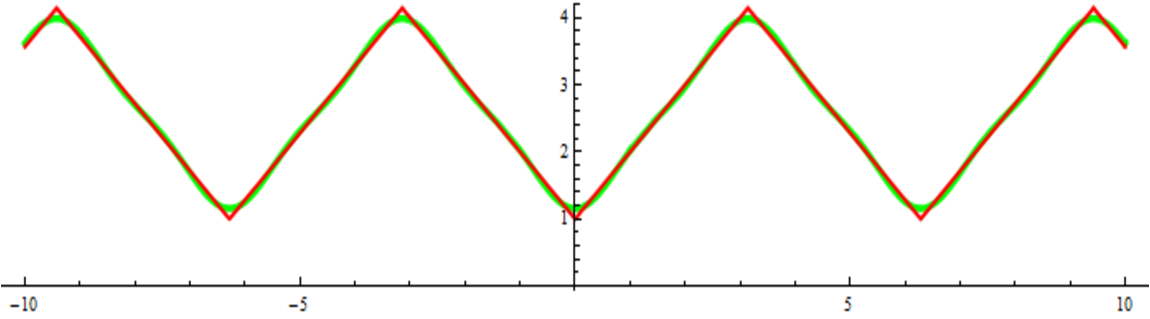
\includegraphics[width=0.8\textwidth]{./images/ch13/cs.pdf} 
	
	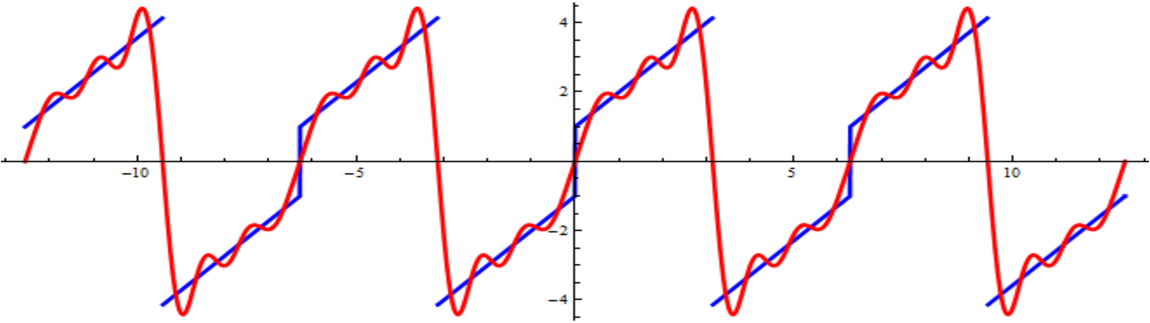
\includegraphics[width=0.8\textwidth]{./images/ch13/ss.pdf}
\end{center}

特别需要注意的是,{\b 对于同一个定义在$(0,\pi)$上的函数,采用不同的延拓方式展开成
三角级数,所得的结果可能是不同的!这和Fourier展开的唯一性并不矛盾,因为
对于延拓后生成的函数来说,其对应的Fourier级数是唯一的。}

{\bf 例:}设$f(x)=\pi x-x^2\,(0<x<\pi)$,又设$S(x)$是$f(x)$在$(0,\pi)$内以
$2\pi$为周期的正弦级数展开式的和函数,求当$x\in(\pi,2\pi)$时$S(x)$的表达式。

\subsection{周期为$2l$的Fourier级数}

接下来考虑任意周期为$2l$的函数$f(x)$的三角级数展开问题,其中$l\ne0$且不一定等于$\pi$。

从数学的角度,只需通过一些坐标的伸缩即可达到展开的目的。具体来说,令$t=\df{\pi}{l}x$,
则$g(t)=f\left(\df{l}{\pi}t\right)$ 是以$2\pi$为周期的函数。 
对$g(t)$做Fourier展开,由其展开式可变换得到$f(x)$的展开式。

\begin{thx}
	{\bf 以$2l$为周期的函数的Fourier展开:}
	$$f(x)=\df{a_0}2+\sumn\left(a_n\cos\df{n\pi}lx+b_n\sin\df{n\pi}lx\right)$$
	其中
	$$\left\{\begin{array}{ll}
	a_n=\df1{l}\dint_{-l}^{l}f\left(\df{\pi}lx\right)
	\cos n\left(\df{\pi}lx\right)\d x,\;&
	n=0,1,2,\ldots\\[5pt] b_n=\df1{l}\dint_{-l}^{l}f\left(\df{\pi}lx\right)
	\sin n\left(\df{\pi}lx\right)\d x,\;& n=1,2,\ldots
	\end{array}\right.$$
\end{thx}

需要注意的是,此时得到的$f(x)$的展开式,其基函数并不是以$2\pi$为周期的三角函数,
而是以$2l$为周期的三角函数。

{\bf 例:}将函数$f(x)=x\,(0<x<1)$表示为只有余弦项的三角级数,写出其和函数,
并求$S(2017.6)$的值。

\begin{shaded}
	{\bf 复数形式的Fourier级数}
	
	在工程实际中,复数形式的Fourier级数应用更加广泛:设$f(x)$以$2l\,(l>0)$为
	周期,则在$f(x)$的连续点上,总有
	$$f(x)=\df1{2l}\sumn[-\infty]e^{\frac{n\pi x}li}
	\dint_{-l}^lf(x)e^{-\frac{n\pi x}li}\d x,$$
	其中$i=\sqrt{-1}$表示虚数单位。
\end{shaded}

\begin{ext}
	{\bf 课后作业}
	\begin{enumerate}
	  \item 将下列函数展成Fourier级数
		\begin{enumerate}[(1)]
% 		  \setlength{\itemindent}{1cm}
		  \item $f(x)=\sin^4x$
		  \item $f(x)=\arcsin(\sin x)$
		\end{enumerate}
% 	  \item 设$f(x)$是以$2\pi$为周期的连续函数,在$[-\pi,\pi]$上满足Dirichlet条件,
% 		且其Fourier系数为$a_k,b_k$。设
% 		$$G(x)=\df1{\pi}\dint_{-\pi}^{\pi}f(t)f(x+t)dt$$
% 		\begin{enumerate}[(1)]
% % 		  \setlength{\itemindent}{1cm}
% 		  \item 证明$G(x)$为偶函数
% 		  \item 求$G(x)$的Fourier系数
% 		  \item 证明$\df1{\pi}\dint_{-\pi}^{\pi}f^2(x)dx=\df{a_0^2}2+
% 		  \sum\limits_{k=1}^{\infty}(a_k^2+b_k^2)$
% 		\end{enumerate}
	  \item 分别写出$f(x)=1-\df{x}{\pi}\;(0\leq x<\pi)$的正弦和余弦级数的和函数$S(x)$,
		并求$S(-3)$和$S(12)$。
	  \item 写出$f(x)=\left\{\begin{array}{ll}
			-\df12x,&-\pi<x<0\\ x-\pi,&0\leq x\leq \pi
		\end{array}\right.$的Fourier级数的和函数$S(x)$,并求$S(100)$和$S(-31.4)$。
	  \item 已知$f(x)=\left\{\begin{array}{ll}
			x^2,&0<x<1/2\\ 1-x,&1/2\leq x\leq 1
		\end{array}\right.$,
		$S(x)=\df{a_0}2+\sumn a_n\cos n\pi,\;(x\in\mathbb{R})$,其中
		$a_n=2\dint_0^1\cos n\pi\d x\;(n=0,1,2,\ldots)$,求$S(2017)$和$S(2017.5)$。
	\end{enumerate}
\end{ext}

\newpage

\section*{作业参考解答}
% \addcontentsline{toc}{section}{作业参考解答}

\begin{center}
	\bf 12.1 数项级数的概念与性质
\end{center}

\bs

1.求以下级数的和

(1)$\df1{1\cdot6}+\df1{6\cdot11}+\df1{11\cdot16}+\ldots$

[解]:
\begin{align*}
	\mbox{原式}
	&=\df15\left(1-\df16+\df16-\df1{11}+\df1{11}-\df1{16}+\ldots\right)\\
	&=\df15\limn\left(1-\df1{5n+1}\right)=\df15.
\end{align*}

(2)$\df1{1\cdot2\cdot3}+\df1{2\cdot3\cdot4}+\df1{3\cdot4\cdot5}+\ldots$

[解]:
\begin{align*}
	\mbox{原式}
	&=\df12\left(1-\df22+\df13+\df12-\df23+\df14
	+\df13-\df24+\df15+\ldots\right)\\
	&=\df12\limn\left(1-\df12-\df1{n}+\df1{n+1}\right)
	=\df14.
\end{align*}

(3)$\sumn\df{n}{(n+1)!}$
[解]:
$$
\mbox{原式}
=\limn\sumk{1}\left[\df1{n!}-\df1{(n+1)!}\right]
=\limn\left(1-\df1{(n+1)!}\right)=1.$$
\fin

\bs

2.已知$\sumn(a_{2n-1}+a_{2n})$收敛,能否推出$\sumn a_n$收敛?
如果能,请给出证明;如果不能,请给出反例,并讨论还需要增加什么条件才能够由
前者推出后者。

[答]:已知$\sumn(a_{2n-1}+a_{2n})$收敛,不能推出$\sumn a_n$收敛。

考虑$a_n=(-1)^{n+1}$,显然$\sumn a_n$发散,但由于对任意$n$,都有
$a_{2n-1}+a_{2n}\equiv0$,故级数$\sumn(a_{2n-1}+a_{2n})$收敛。

可以证明,如果同时满足$\limn a_n=0$,则由$\sumn(a_{2n-1}+a_{2n})$收敛,
可以推出$\sumn a_n$收敛。事实上,记$\{S_n\}$为$\sumn a_n$的部分和数列,
则由$\sumn(a_{2n-1}+a_{2n})$收敛可知,$\{S_{2n}\}$必收敛,设其极限
为$S$,则
$$S_{2n+1}=S_{2n}+a_{2n+1}\to S+0=S,\;(n\to\infty)$$
从而由拉链定理,可知$\{S_n\}$收敛,也即$\sumn a_n$收敛。\fin

3.利用Cauchy审敛原理判定如下级数的敛散性

(1)$\sumn\df{(-1)^{n}}n$

[证]:对任意$\e>0$,令$N=\left[\df1{\e}\right]+1$,则对任意$m>n>N$,
若$m-n$为偶数,则有
\begin{align*}
	\left|\sum\limits_{k=n}^m\df{(-1)^{k}}k\right|
	&=\df1n-\left(\df1{n+1}-\df1{n+2}\right)
	-\left(\df1{n+3}-\df1{n+4}\right)\\
	&-\ldots
	-\left(\df1{m-2}-\df1{m-1}\right)-\df1m\\
	&<\df1n-\df1m<\df1n<\e
\end{align*}
若$m-n$为奇数,则有
\begin{align*}
	\left|\sum\limits_{k=n}^m\df{(-1)^{k}}k\right|
	&=\df1n-\left(\df1{n+1}-\df1{n+2}\right)
	-\left(\df1{n+3}-\df1{n+4}\right)\\
	&-\ldots-\left(\df1{m-1}-\df1m\right)\\
	&<\df1n<\e
\end{align*}
从而由Cauchy审敛原则,可知该级数收敛。

(2)$\sumn\df{\sin nx}{2^n}$

[证]:对任意$\e>0$,令$N=\left[-\log_2\e\right]+2$,则对任意$m>n>N$,
$$
	\left|\sum\limits_{k=n}^m\df{\sin kx}{2^k}\right|
	\leq\sum\limits_{k=n}^m\left|\df{\sin kx}{2^k}\right|
	\leq\sum\limits_{k=n}^m\left|\df1{2^k}\right|
	\leq\df1{2^{N-1}}<\e,
$$
从而由Cauchy审敛原则,可知该级数收敛。\fin

\begin{center}
	\bf 12.2 数项级数的审敛法
\end{center}

\bs

1.判断以下级数的敛散性,如果是收敛的变号级数,说明其是绝对收敛还是条件收敛:

(1)$\sumn\df{n-2}{3n^2+n}$

[解]:
$$\limn n\df{n-2}{3n^2+n}=\df13>0,$$
又$\sumn\df1n$发散,故由比较判别法可知,原级数发散。

(2)$\sumn\df{\sqrt{n+2}-\sqrt{n}}{\sqrt{n+1}}$

[解]:
$$\limn n\df{\sqrt{n+2}-\sqrt{n}}{\sqrt{n+1}}=1>0,$$
又$\sumn\df1n$发散,故由比较判别法可知,原级数发散。

(3)$\sumn\df{4^n}{n\cdot 3^n}$

[解]:
$$\limn\sqrt[n]{\df{4^n}{n\cdot 3^n}}=\df43>1,$$
故由根植判别法可知,原级数发散。

(4)$\sumn\df{n^2}{3^n}$

[解]:
$$\limn\sqrt[n]{\df{n^2}{3^n}}=\df13<1,$$
故由根植判别法可知,原级数收敛。

(5)$\sumn\df1n\arctan\df1{n-1}$

[解]:
$$\limn n^2\df1n\arctan\df1{n-1}=1>0,$$
又$\sumn\df1{n^2}$收敛,故由比较判别法可知,原级数收敛。

(6)$\sumn\left(\df{n}{2n-1}\right)^{3n+2}$

[解]:
$$\limn\sqrt[n]{\left(\df{n}{2n-1}\right)^{3n+2}}=\df18<1,$$
故由根植判别法可知,原级数收敛。

(7)$\sumn n\left(\df34\right)^n$

[解]:
$$\limn \sqrt[n]{n\left(\df34\right)^n}=\df34<1,$$
故由根植判别法可知,原级数收敛。

(8)$\sumn\df{n^2}{n!}$

[解]:
$$\limn\df{\df{(n+1)^2}{(n+1)!}}{\df{n^2}{n!}}=0<1,$$
故由比值判别法可知,原级数收敛。

(9)$\sumn\df{n^{n+\frac1n}}{\left(1+\df1n\right)^n}$

[解]:
$$\df{n^{n+\frac1n}}{\left(n+\df1n\right)^n}\geq\df{n^n\cdot
n^{\frac1n}}{(n+1)^n}\to\df1e,\;(n\to\infty),$$
由此可知该级数不满足级数收敛的必要条件,故该级数发散。

(10)$\sumn(-1)^n\df{2^n}{n!}$

[解]:
$$\limn\df{\df{2^{n+1}}{(n+1)!}}{\df{2^n}{n!}}=0<1,$$
故由比值判别法,可知$\sumn\df{2^n}{n!}$,从而
$\sumn(-1)^n\df{2^n}{n!}$绝对收敛。

(11)$\sumn\sin\left(\pi\sqrt{n^2+1}\right)$

[解]:
$$\sin\left(\pi\sqrt{n^2+1}\right)=(-1)^n
\sin\left(\df{\pi}{\sqrt{n^2+1}+n}\right),$$
注意到$\sin\left(\df{\pi}{\sqrt{n^2+1}+n}\right)$单调递减趋于零,
故由Leibniz判别法,原级数收敛。又
$$\limn n\sin\left(\df{\pi}{\sqrt{n^2+1}+n}\right)=\df12>0,$$
而$\sumn\df1n$发散,故由比较判别法,$\sumn\left|\sin
\left(\pi\sqrt{n^2+1}\right)\right|$发散。综上,该级数条件收敛。

(12)$\sumn\dint_0^{\frac{\pi}n}\df{\sin x}{1+x}\d x$

[解]:
$$\limn n^2\dint_0^{\frac{\pi}n}\df{\sin x}{1+x}\d x
=\lim\limits_{y\to0}\df{\dint_0^{{\pi}y}\df{\sin x}{1+x}\d x}{y^2}
=\df{\pi}2>0,$$
又$\sumn\df1{n^2}$收敛,故由比较判别法可知,原级数收敛。

(13)$\sumn\df{2^n-n^2}{3^n}$

[解]:
$$\limn\sqrt[n]{\df{2^n-n^2}{3^n}}=\df23<1,$$
故由根植判别法可知,原级数收敛。

(14)$\sumn\df1{n\ln^2(n+1)}$

[解]:$n>2$时,
$$\df1{n\ln^2(n+1)}<\df1{n\ln^2n},$$
注意到无穷积分
$$\dint_2^{+\infty}\df1{x\ln^2x}\d x
=\left.-\df1{\ln x}\right|_2^{+\infty}=\ln2,$$
收敛,故由积分判别法,可知$\sumn\df1{n\ln^2n}$,进而由比较判别法,可知
原级数收敛。\fin

\bs

2.判断以下命题的正误,如果正确,证明之;如果错误,请给出反例,并讨论
需要添加什么条件方能使之成立:

(1)已知级数$\sumn a_n$收敛,则级数$\sumn a^2_n$收敛;

[答]:不成立,例如$a_n=\df{(-1)^n}{\sqrt n}$,由Leibniz判别法可知,
该级数收敛。又$a_n^2=\df1n$,而$\sumn\df1n$发散。

若同时有$\sumn a_n$为正项级数,则以上命题成立。事实上,由$\sumn a_n$收敛,
必有$\limn a_n=0$,进而
$$\limn\df{a_n^2}{a_n}=0,$$
从而由比较判别法可知,级数$\sumn a^2_n$收敛。

(2)已知级数$\sumn a^2_n$收敛,则级数$\sumn a^3_n$收敛;

[答]:该命题成立。事实上,由$\sumn a^2_n$收敛,可知$\limn a_n^2=0$,
进而易知$\limn a_n=0$,于是
$$\limn\df{|a_n^3|}{a_n^2}=\limn|a_n|=0<1,$$
从而由比较判别法,$\sumn|a_n^3|$收敛,进而$\sumn a^3_n$收敛。

(3)正项级数$\sumn a_n$与级数$\sumn\df{a_n}{1+a_n}$同敛散;

[答]:该命题成立。事实上,若$\sumn a_n$收敛,则必有$\limn a_n=0$,
从而
$$\limn\df{a_n}{\df{a_n}{1+a_n}}=1>0,$$
于是由比较判别法可知,$\sumn\df{a_n}{1+a_n}$收敛。

另一方面,记$b_n=\df{a_n}{1+a_n}$,则
$a_n=\df{b_n}{1-b_n}$。若$\sumn b_n$收敛,则必有$\limn b_n=0$,
从而
$$\limn\df{\df{b_n}{1-b_n}}{b_n}=1>0,$$
于是由比较判别法可知,$\sumn a_n$收敛。

(4)对于正项级数$\sumn a_n$,若当$n$充分大时,总有$\df{a_{n+1}}{a_n}<1$,
则该级数收敛。

[答]:不成立。考虑$a_n=\df1n$,显然对任意$n$,均有$\df{a_{n+1}}{a_n}<1$,
但$\sumn a_n=\sum\df1n$发散。

若条件改为“当$n$充分大时,总有$\df{a_{n+1}}{a_n}<q<1$”,则该命题即为
比值判别法的不等式形式,必然成立。
\fin

\begin{center}
	\bf 12.3 幂级数及其应用
\end{center}

1.求下列函数项级数的收敛域

(1)$\df x{1\cdot 3}+\df{x^2}{2\cdot3^2}++\df{x^3}{3\cdot3^3}
+\ldots++\df{x^n}{n\cdot3^n}+\ldots$

[解]:因为
$$\limn\sqrt[n]{\df1{n\cdot 3^n}}=\df13,$$
故该级数的收敛区间为$(-3,3)$。

又$x=3$时,级数为$\sumn\df1n$,发散;
$x=-3$时,级数为$\sumn\df{(-1)^n}n$,收敛。
故所求收敛域为$[-3,3)$。

(2)$\sumn\df{(2x+1)^n}n$

[解]:令$y=2x+1$,考虑级数$\sumn\df{y^n}n$。因为$\limn\sqrt[n]{\df1n}=1$,
故其收敛区间为$(-1,1)$。

又$y=1$时,级数为$\sumn\df1n$,发散;
$y=-1$时,级数为$\sumn\df{(-1)^n}n$,收敛。故级数$\sumn\df{y^n}n$
的收敛域为$y\in[-1,1)$。相应地,原级数的收敛域为$x\in[-1,0)$。

(3)$\sumn(-1)^n\df{x^{2n+1}}{2n}$

[解]:$\sumn(-1)^n\df{x^{2n+1}}{2n}=x\cdot\sumn(-1)^n\df{x^{2n}}{2n}$,
由此可知原级数与级数$\sumn(-1)^n\df{x^{2n}}{2n}$同敛散。

令$y=x^2$,考虑级数$\sumn(-1)^n\df{y^{n}}{2n}$。因为
$\limn\sqrt[n]{\df1{2n}}=1$,故该级数的收敛区间为$(-1,1)$。
相应地,级数$\sumn(-1)^n\df{x^{2n}}{2n}$与原级数的收敛区间均为$(-1,1)$。

又$x=\pm1$时,原级数为$\sumn\df{(-1)^n}{2n}$,由Leibniz判别法,收敛。
故原级数的收敛域为$[-1,1]$。

(4)$\sumn\sin\df 1 {3n}\left(\df{3+x}{3-2x}\right)^n$

[解]:令$y=\df{3+x}{3-2x}$,考虑级数$\sumn y^n\sin\df1{3n}$。
因为
$$\limn\df{\sin\frac1{3n}}{\sin\frac1{3(n+1)}}=1,$$
故该级数的收敛区间是$(-1,1)$。

又$y=1$时,级数为$\sumn\sin\df1{3n}$,因为$\limn n\sin\df1{3n}=\df13$,
故由比较判别法,级数发散;$y=-1$时,级数为$\sumn(-1)^n\sin\df1{3n}$,
由Leibniz判别法,收敛。故级数$\sumn y^n\sin\df1{3n}$的收敛域为
$[-1,1)$。求解不等式
$$-1\leq\df{3+x}{3-2x}<1$$
可得$x\in(-\infty,0)\cup[6,+\infty)$,即为所求原级数的收敛域。\fin

\bs

2.求下列级数的和函数

(1)$\sumn(-1)^{n-1}nx^{n-1}$

[解]:令$y=-x$,考虑级数$\sumn ny^{n-1}$,易得该级数的收敛域为$(-1,1)$。
设其和函数为$S(y)$,于是当$y\in(-1,1)$时,
$$\dint_0^yS(t)\d t=\dint_0^y\sumn nt^{n-1}\d t
=\sumn \dint_0^ynt^{n-1}\d t=\sumn y^n=\df1{1-y}-1,$$
进而可得
$$S(y)=\df1{(1-y)^2}.$$

综上,
$$\sumn(-1)^{n-1}nx^{n-1}=\df1{(1+x)^2},\quad x\in(-1,1).$$

(2)$\df1a+\df{2x}{a^2}+\ldots+\df{nx^{n-1}}{a^n}+\ldots$,其中$a>0$.

[解]:
该级数即为$\df1a\sumn n\left(\df xa\right)^{n-1}$,易得其收敛域为$(-a,a)$。
记$y=\df xa$,由(1)的结果可得
$$\df1a\sumn n\left(\df xa\right)^{n-1}
=\df1a\sumn ny^{n-1}=\df1a\df1{(1-y)^2}=\df1a\df1{\left(1-\frac xa\right)^2}
=\df{a}{(a-x)^2}.$$
即为所求。

(3)$\sumn[0]\df{x^{2n+1}}{n!}$

[解]:该级数的收敛域为$(-\infty,+\infty)$。令$y=x^2$
$$\sumn[0]\df{x^{2n+1}}{n!}=x\sumn[0]\df{x^{2n}}{n!}
=x\sumn[0]\df{y^n}{n!}.$$
级数$\sumn[0]\df{y^n}{n!}$当$y\in(-\infty,+\infty)$时收敛于$e^y$。
由此即知
$$\sumn[0]\df{x^{2n+1}}{n!}=xe^{x^2},\quad x\in(-\infty,+\infty).$$
\fin

\bs

3.将下列函数展开成Maclaurin级数,并求其收敛域

% (1)$f(x)=\arcsin x$
% 
% [解]:
% \begin{align*}
% 	f'(x)&=\df1{\sqrt{1-x^2}}=(1-x^2)^{-\frac12}\\
% 	&=\sumn[0]\df{\left(\begin{array}{c}
% 		-\frac12 \\ n
% 	\end{array}\right)}{n!}(-x^2)^n
% 	=\sumn[0]\df{(2n-1)!!}{(2n)!!}x^{2n},
% \end{align*}
% 注意到
% $$\limn\df{\frac{(2n+1)!!}{(2n+2)!!}}{\frac{(2n-1)!!}{(2n)!!}}=1,$$
% 故级数$\sumn[0]\df{(2n-1)!!}{(2n)!!}x^{2n}$的收敛区间为
% $(-1,1)$
% 右端
% 于是,在右端级数的收敛域内有
% $$f(x)=\dint_0^x\sumn[0]\df{(2n-1)!!}{(2n)!!}t^{2n}\d t
% =$$

(1)$f(x)=\df1{x^2-4x+3}$

[解]:
\begin{align*}
	\df1{x^2-4x+3}&=\df12\left(\df1{1-x}-\df13\df1{1-\frac x3}\right)\\
	&=\df12\left(\sumn[0]x^n-\df13\sumn[0]\df{x^n}{3^n}\right)\\
	&=\df12\sumn[0]\left(1-\df1{3^{n+1}}\right)x^n.
\end{align*}
该级数的收敛域为$[-1,1)$。

(2)$f(x)=\df 1{1+x+x^2}$

[解]:
\begin{align*}
	\df 1{1+x+x^2}
	&=\df{1-x}{1-x^3}=(1-x)\sumn[0]x^{3n}\\
	&=1-x+x^3-x^4+x^6-x^7+\ldots+x^{3n}-x^{3n+1}+\ldots.
\end{align*}
注意到级数$\sumn[0]x^{3n}$的收敛域为$(-1,1)$,故以上级数的收敛域为$(-1,1)$。\fin

\bs

4.将函数$f(x)=\df1{\sqrt{3+2x-x^2}}$展开成$x=1$处的幂级数,并求其收敛区间。

[解]:
\begin{align*}
	f(x)
	&=\df12\left[1-\left(\df{x-1}2\right)^2\right]^{-\frac12}
	=\df12\sumn[0]{\left(\begin{array}{c}
		-\frac12 \\ n
	\end{array}\right)}\left[-\left(\df{x-1}2\right)^2\right]^n\\
	&=\sumn[0]\df{(2n-1)!!}{2^{2n+1}(2n)!!}(x-1)^{2n}
\end{align*}
注意到
$$\limn\df{\df{(2n+1)!!}{2^{2n+3}(2n+2)!!}}{\df{(2n-1)!!}{2^{2n+1}(2n)!!}}=\df12,$$
故所得级数的收敛半径为$2$,相应地收敛区间为$(-1,3)$。
\fin

\bs

5.已知$f_n(x)\;(n\in\mathbb{Z}^+)$满足
$$f'_n(x)=f_n(x)+x^{n-1}e^x,$$
且$f_n(1)=\df en$,求级数$\sumn f_n(x)$的和。

[解]:由已知等式,可得
$$\left[f_n(x)e^{-x}\right]'=x^{n-1},$$
进而可知
$$f_n(x)=\left(\df{x^n}n+C\right)e^x.$$
注意到$f_n(1)=\df en$,可得$C=0$,故$f_n(x)=\df{x^n}ne^x$。

$$\sumn f_n(x)=\sumn\df{x^n}ne^x=e^x\sumn\df{x^n}n.$$
	
考虑级数$\sumn\df{x^n}n$,易得其收敛域为$[-1,1)$。设其和函数为$S(x)$,则
$$S'(x)=\left[\sumn\df{x^n}n\right]'
=\sumn\left[\df{x^n}n\right]'=\sumn x^{n-1}=\df1{1-x}.$$
从而
$$S(x)=\dint_0^x\df1{1-t}\d t=-\ln|1-x|,\quad x\in[-1,1),$$
进而
$$\sumn f_n(x)=-e^x\ln|1-x|,\quad x\in[-1,1).$$
\fin

\bs

6.参考{\kaishu 同济教材第十二章第五节“一、近似计算”}的内容,
用幂级数计算下列各数的近似值:

(1)$\sqrt[3]e$,误差不超过$10^{-3}$

[解]:
$$e^x=\sumn[0]\df{x^n}{n!},\;x\in\mbb{R}.$$
当$|x|<1$时,展开到第$n$项的误差
\begin{align*}
	r_n&=\sum\limits_{k=n+1}^{\infty}\df{x^k}{k!}\\
	&=\df{x^{n+1}}{(n+1)!}\left[1+\df{x}{n+2}+\df{x^2}{(n+2)(n+3)}+\ldots\right]\\
	&<\df{x^{n+1}}{(n+1)!}(1+x+x^2+\ldots)=\df{x^{n+1}}{(n+1)!(1-x)},
\end{align*}
带入$x=\df13$,令$|r_n|\leq 10^{-3}$,可以推出$n\geq 3$,故所求结果
$$
\sqrt[3]e\approx1+\df13+\df{\frac1{3^2}}2+\df{\frac1{3^3}}{3!}
=\df{113}{81}\approx=1.395.
$$

(2)计算$\dint_0^{\frac12}\df{\arctan x}x\d x$的近似值,
误差不超过$10^{-3}$。

[解]:注意到
$$(\arcsin x)'=(1-x^2)^{-\frac12}
=\sumn[0]\df{(2n-1)!!}{(2n)!!}x^{2n},\quad x\in(-1,1),$$
故
$$\arcsin x=\sumn[0]\df{(2n-1)!!}{(2n)!!(2n+1)}x^{2n+1},\quad x\in(-1,1),$$
进而
$$\dint_0^{\frac12}\df{\arcsin x}x\d x
=\sumn[0]\df{(2n-1)!!}{(2n)!!(2n+1)^2}\df1{2^{2n+1}},$$
估计误差
\begin{align*}
	\left|r_n\left(\df12\right)\right|
	&=\sum\limits_{k=n+1}^{\infty}\df{(2k-1)!!}
	{(2k)!!(2k+1)^2}\df1{2^{2k+1}}\\
	&<\df{(2n+1)!!}{(2n+2)!!(2n+3)^22^{2n+3}}
	\left[1+\df1{2^2}+\df1{2^4}+\ldots\right]\\
	&<\df{(2n+1)!!}{(2n+2)!!(2n+3)^22^{2n+2}}.
\end{align*}
当$n=2$时,$r_n\left(\df12\right)=\df{15}{25088}<10^{-3}$,故所求近似值为
$$\df12+\df1{2\cdot3^2\cdot2^3}+\df{1\cdot3}{2\cdot4\cdot5^2\cdot32^2}
=\df{29227}{57600}\approx0.5074.$$
\fin 

\begin{center}
	\bf 12.4 Fourier级数
\end{center}

1.将下列函数展成Fourier级数

(1)$f(x)=\sin^4x$

[解]:三角多项式的Fourier级数是其自身,
\begin{align*}
	\sin^4x&=\left(\df{1-\cos2x}2\right)^2
	=\df14\left(1-2\cos2x+\cos^22x\right)\\
	&=\df14\left(1-2\cos2x+\df{1+\cos4x}2\right)
	=\df38-\df12\cos2x+\df18\cos4x
\end{align*}
最后的展开式即为所求。

(2)$f(x)=\arcsin(\sin x)$

[解]:
$$\arcsin(\sin x)=\left\{\begin{array}{ll}
	-x-\pi, & x\in\left[-\pi,-\frac{\pi}2\right)\\
	x, & x\in\left[-\frac{\pi}2,\frac{\pi}2\right)\\
	-x+\pi, & x\in\left[\frac{\pi}2,\pi\right)
\end{array}\right.$$
注意到该函数为奇函数,故其Fourier展开式中$a_n=0,n=0,1,2,\ldots$,
\begin{align*}
	b_n&=\df2{\pi}\dint_0^{\pi}f(x)\d x
	=\df2{\pi}\dint_0^{\frac{\pi}2}x\sin nx\d x
	+\df2{\pi}\dint_{\frac{\pi}2}^{\pi}(-x+\pi)\sin nx\d x\\
	&=\left\{\begin{array}{ll}
		0, & n=2k,\\ \df{4(-1)^k}{\pi(2k+1)^2}, & n=2k+1.
	\end{array}\right.
\end{align*}
故所求Fourier级数为
$$f(x)\sim\sumn[0]\df{4(-1)^n}{\pi(2n+1)^2}\sin(2n+1)x.$$
\fin

\bs

2.分别写出$f(x)=1-\df{x}{\pi}\;(0\leq x\leq\pi)$的正弦和余弦级数的和函数$S(x)$,
并求$S(-3)$和$S(12)$。

[解]:$f(x)$对应的正弦级数的和函数为
$$S_1(x)=\left\{\begin{array}{ll}
	-1-\frac x{\pi}, & x\in[-\pi,0),\\
	1-\frac x{\pi}, & x\in(0,\pi),\\
	0, & x=0,\\
	S_1(x+2\pi), & \mathrm{else}.
\end{array}\right.$$
于是
$$S_1(-3)=-1+\df3{\pi},\quad
S_1(12)=S_1(12-4\pi)=3-\df{12}{\pi}.$$

$f(x)$对应的余弦级数的和函数为
$$S_2(x)=\left\{\begin{array}{ll}
	1+\frac x{\pi}, & x\in[-\pi,0),\\
	1-\frac x{\pi}, & x\in[0,\pi),\\
	S_2(x+2\pi), & \mathrm{else}.
\end{array}\right.$$
相应地,
$$S_2(-3)=1-\df3{\pi},\quad
S_2(12)=-3+\df{12}{\pi}.$$
\fin

3.写出$f(x)=\left\{\begin{array}{ll}
	-\df12x,&-\pi<x<0\\ x-\pi,&0\leq x\leq \pi
\end{array}\right.$的Fourier级数的和函数$S(x)$,并求$S(100)$和$S(-31.4)$。

[解]:
$$S(x)=\left\{\begin{array}{ll}
	\frac{\pi}4, & x=-\pi,\\
	-\frac12x, & x\in(-\pi,0),\\
	\frac{\pi}2, & x=0,\\
	x-\pi, & x\in(0,\pi),\\
	S_2(x+2\pi), & \mathrm{else}.
\end{array}\right.$$
于是
$$S(100)=S(100-32\pi)=16\pi-50,\quad
S(-3.14)=1.57.$$
\fin

\bs

4.已知$f(x)=\left\{\begin{array}{ll}
	x^2,&0<x<1/2\\ 1-x,&1/2\leq x\leq 1
\end{array}\right.$,
$S(x)=\df{a_0}2+\sumn a_n\cos n\pi,\;(x\in\mathbb{R})$,其中
$a_n=2\dint_0^1\cos n\pi\d x\;(n=0,1,2,\ldots)$,求$S(2017)$和$S(2017.5)$。

[解]:
$$S(x)=\left\{\begin{array}{ll}
	x+1, & x\in\left[-1,-\frac12\right),\\
	\frac38, & x=\pm\frac12,\\
	x^2, & |x|<\frac12,\\
	1-x, & x\in\left(\frac12,1\right),\\
	S_2(x+2\pi), & \mathrm{else}.
\end{array}\right.$$
于是
$$S(2017)=S(-1)=0,\quad
S(2017.5)=S(-0.5)=\df38.$$
\fin

\newpage

{\bf 例:}设$f(x)$是以$2\pi$为周期的连续函数,在$[-\pi,\pi]$上满足Dirichlet条件,
且其Fourier系数为$a_k,b_k$。设
$$G(x)=\df1{\pi}\dint_{-\pi}^{\pi}f(t)f(x+t)dt$$
\begin{enumerate}[(1)]
% 		  \setlength{\itemindent}{1cm}
  \item 证明$G(x)$为偶函数
  \item 求$G(x)$的Fourier系数
  \item 证明$\df1{\pi}\dint_{-\pi}^{\pi}f^2(x)dx=\df{a_0^2}2+
  \sum\limits_{k=1}^{\infty}(a_k^2+b_k^2)$
\end{enumerate}

[解]:(1)注意到$f(x)$以$2\pi$为周期,令$y=-x+t$,则对任意$x\in\mbb{R}$,
$$G(-x)=\df1{\pi}\dint_{-\pi}^{\pi}f(t)f(-x+t)\d t
=\df1{\pi}\dint_{-x-\pi}^{-x+\pi}f(x+y)f(y)\d y=G(x),$$
由此即知$G(x)$为偶函数。

(2)因为$G(x)$为偶函数,故在其Fourier级数中,正弦项的系数$B_n=0,n=1,2,\ldots$,
余弦项的系数
\begin{align*}
	A_0&=\df1{\pi^2}\dint_{-\pi}^{\pi}\dint_{-\pi}^{\pi}
	f(t)f(x+t)\d t\d x
	=\df1{\pi^2}\dint_{-\pi}^{\pi}\dint_{-\pi}^{\pi}
	f(x+t)\d x f(t)\d t\\
	&\xlongequal{u=x+t}\df1{\pi^2}\dint_{-\pi}^{\pi}\dint_{t-\pi}^{t+\pi}
	f(u)\d u f(t)\d t
	=\df1{\pi}a_0\dint_{-\pi}^{\pi}f(t)\d t
	=a_0^2\\
	A_n&=\df1{\pi^2}\dint_{-\pi}^{\pi}\dint_{-\pi}^{\pi}
	f(t)f(x+t)\d t\cos nx\d x
	=\df1{\pi^2}\dint_{-\pi}^{\pi}\dint_{-\pi}^{\pi}
	f(x+t)\cos nx\d x f(t)\d t\\
	&\xlongequal{u=x+t}\df1{\pi^2}\dint_{-\pi}^{\pi}\dint_{t-\pi}^{t+\pi}
	f(u)\cos(nu-nt)\d u f(t)\d t\\
	&=\df1{\pi^2}\left[\dint_{-\pi}^{\pi}\dint_{t-\pi}^{t+\pi}
	f(u)\cos nu\d u\cos nt f(t)\d t
	+\dint_{-\pi}^{\pi}\dint_{t-\pi}^{t+\pi}
	f(u)\sin nu\d u\sin nt f(t)\d t\right]\\
	&=\df1{\pi}\left[a_n\dint_{-\pi}^{\pi}f(t)\cos nt\d t
	+b_n\dint_{-\pi}^{\pi}f(t)\sin nt\d t\right]
	=a_n^2+b_n^2.\quad n=1,2,3,\ldots
\end{align*}
综上,$G(x)$的Fourier级数为
$$G(x)\sim\df{a_0^2}2+\sumn(a_n^2+b_n^2)\cos nx.$$

(3)在以上的展开式中,令$x=0$,即得待证等式。\fin